\clearpage

\section{Detailed study of the effect of systematics on the predicted reconstructed energy spectrum of 1 $\mu$-like ring events}
\label{sec:spectrum_systematics}

In this section, the effect of systematics on the predicted reconstructed energy spectrum in SuperK is presented in a number of figures.
Each figure shows the total nominal predicted spectrum (the sum of all SuperK MC modes) and the total spectra resulting from -3$\sigma$, -1$\sigma$, +1$\sigma$, 
and +3$\sigma$ variations of a single systematic parameter.
For correlated systematic parameters, $\sigma$ is defined as the square root of the diagonal entry in the corresponding covariance matrix.
For $\delta_{CP}$, $\sigma$ is taken to be equal to $\pi$.

Figs.\ \ref{fig:noosc_ereco_twk_f_sk_e_scale}-\ref{fig:noosc_ereco_twk_f_skdetfsi005} show the effects of systematics on the SuperK $E_{reco}$ 
spectrum with no oscillations applied (all mixing angles set to zero).
Figs.\ \ref{fig:osc_ereco_twk_sinsqtheta13}-\ref{fig:osc_ereco_twk_f_skdetfsi005} show the effect of systematics on the SuperK $E_{reco}$ spectrum 
with 3-flavour oscillations in matter, using the following values of the oscillation parameters:
\begin{itemize}
\item $\sin^2\theta_{12} = $ 0.306
\item $\sin^2\theta_{13} = $ 0.025
\item $\sin^2\theta_{23} = $ 0.500
\item $\delta_{CP} = $        0
\item $\Delta m^2_{21} = $    7.5$\times$10$^{-5}$ eV$^{2}$/c$^{4}$
\item $|\Delta m^2_{32}| = $  2.4$\times$10$^{-3}$ eV$^{2}$/c$^{4}$.
\end{itemize}
It should be noted that, for ease of comparison, there are only two vertical axis scales used in the lower `ratio' plots. For systematics with a small 
effect, the vertical axis runs from 0.75 to 1.25; for systematics with a larger effect, the vertical axis runs from 0.25 to 1.75.


\begin{figure}
\begin{center}
\resizebox{14cm}{!}{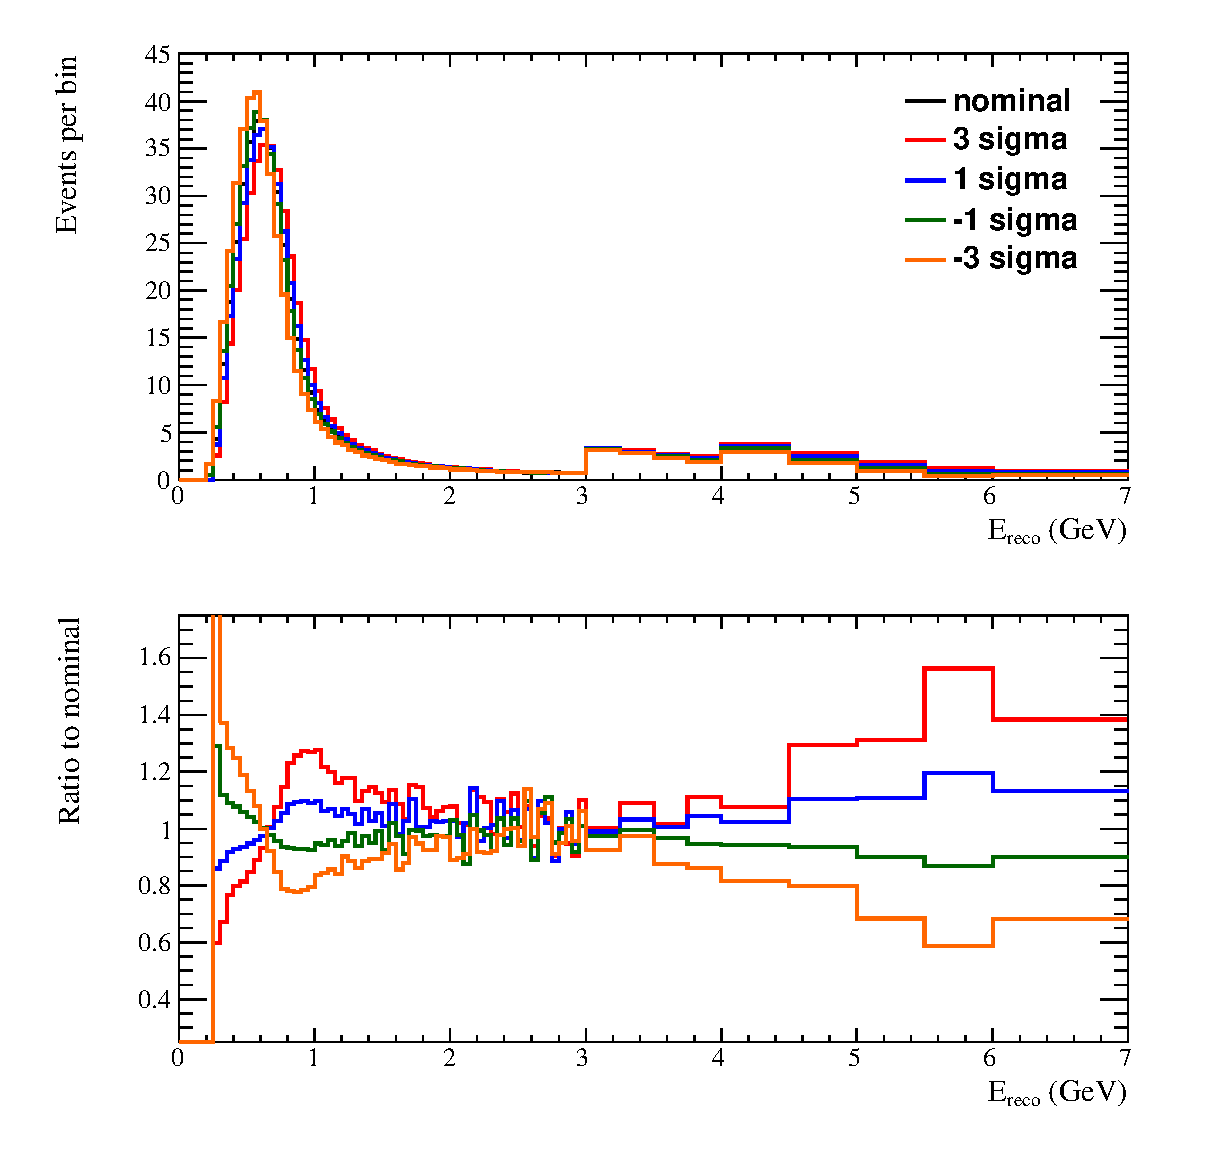
\includegraphics{../images/spectrum_tweaked/1sigma_unoscillated/ereco_twk_f_sk_e_scale}}
\caption
{ Effect of $f_{E; r}^{SK}$   for no oscillations (all mixing angles set to 0). }
\label{fig:noosc_ereco_twk_f_sk_e_scale}
\end{center}
\end{figure}
\clearpage

\begin{figure}
\begin{center}
\resizebox{14cm}{!}{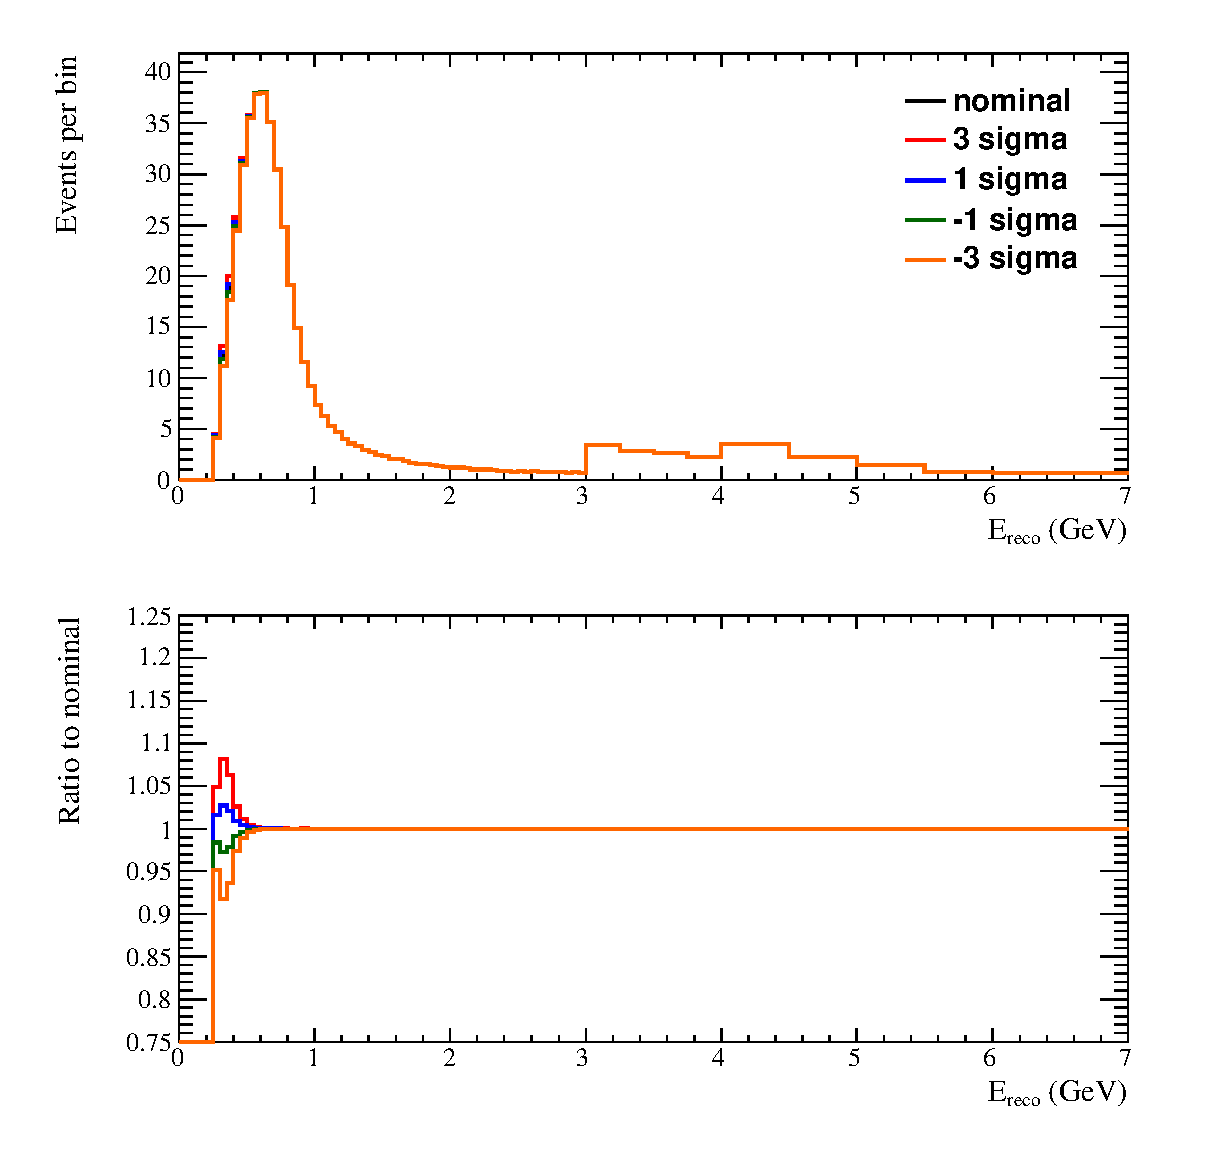
\includegraphics{../images/spectrum_tweaked/1sigma_unoscillated/ereco_twk_f_banff00}}
\caption
{ Effect of $f_{0; t, r}^{banff}$ for no oscillations (all mixing angles set to 0). }
\label{fig:noosc_ereco_twk_f_banff00}
\end{center}
\end{figure}
\clearpage

\begin{figure}
\begin{center}
\resizebox{14cm}{!}{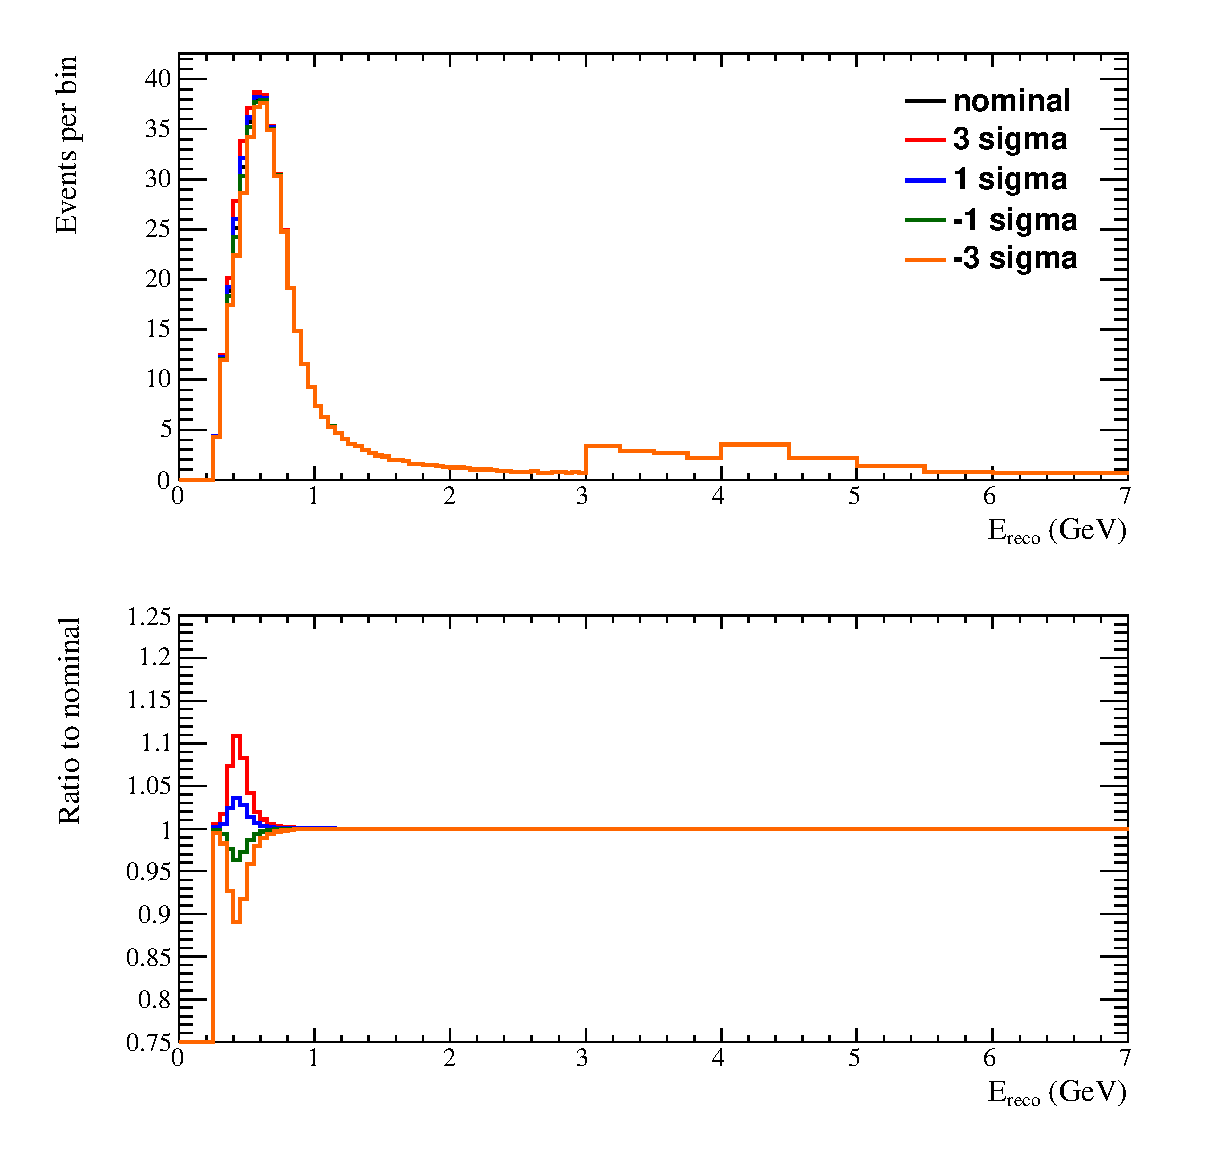
\includegraphics{../images/spectrum_tweaked/1sigma_unoscillated/ereco_twk_f_banff01}}
\caption
{ Effect of $f_{1; t, r}^{banff}$ for no oscillations (all mixing angles set to 0). }
\label{fig:noosc_ereco_twk_f_banff01}
\end{center}
\end{figure}
\clearpage

\begin{figure}
\begin{center}
\resizebox{14cm}{!}{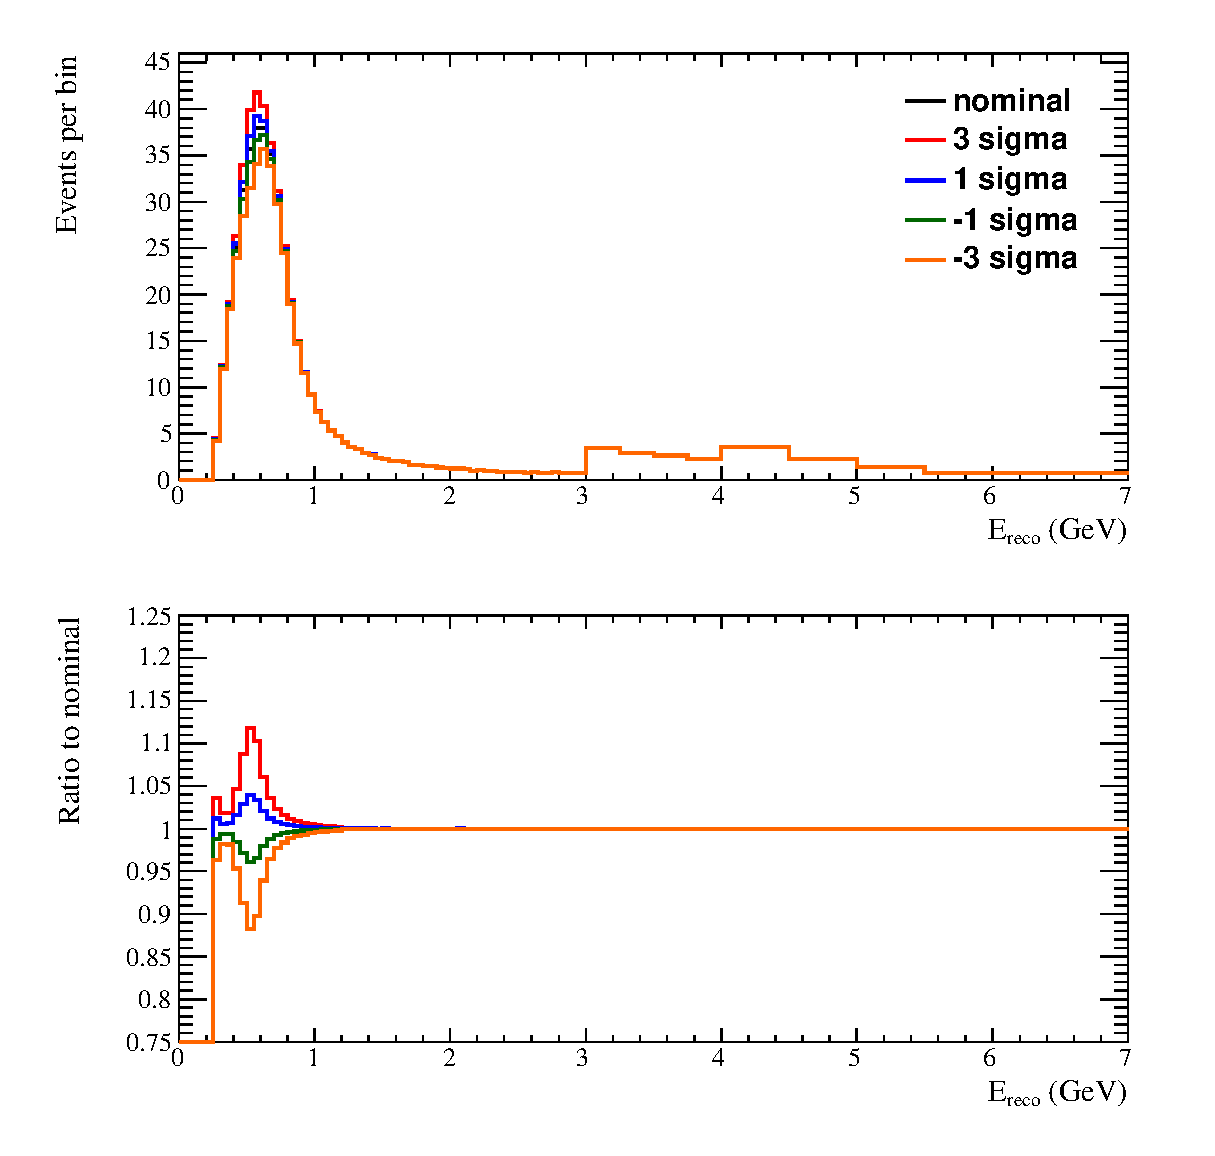
\includegraphics{../images/spectrum_tweaked/1sigma_unoscillated/ereco_twk_f_banff02}}
\caption
{ Effect of $f_{2; t, r}^{banff}$ for no oscillations (all mixing angles set to 0). }
\label{fig:noosc_ereco_twk_f_banff02}
\end{center}
\end{figure}
\clearpage

\begin{figure}
\begin{center}
\resizebox{14cm}{!}{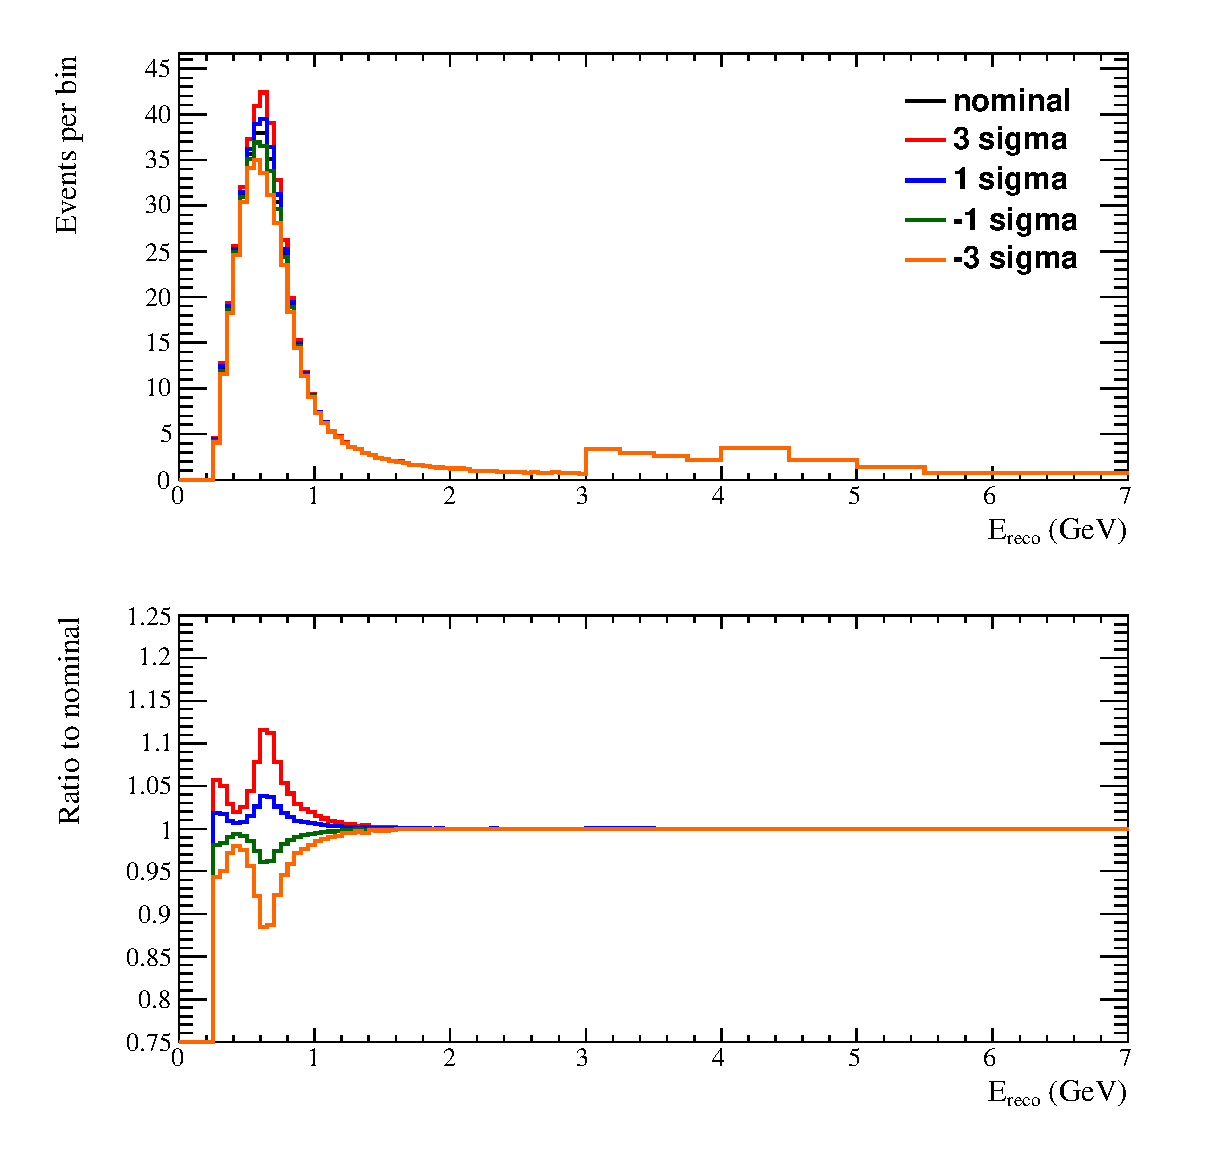
\includegraphics{../images/spectrum_tweaked/1sigma_unoscillated/ereco_twk_f_banff03}}
\caption
{ Effect of $f_{3; t, r}^{banff}$ for no oscillations (all mixing angles set to 0). }
\label{fig:noosc_ereco_twk_f_banff03}
\end{center}
\end{figure}
\clearpage

\begin{figure}
\begin{center}
\resizebox{14cm}{!}{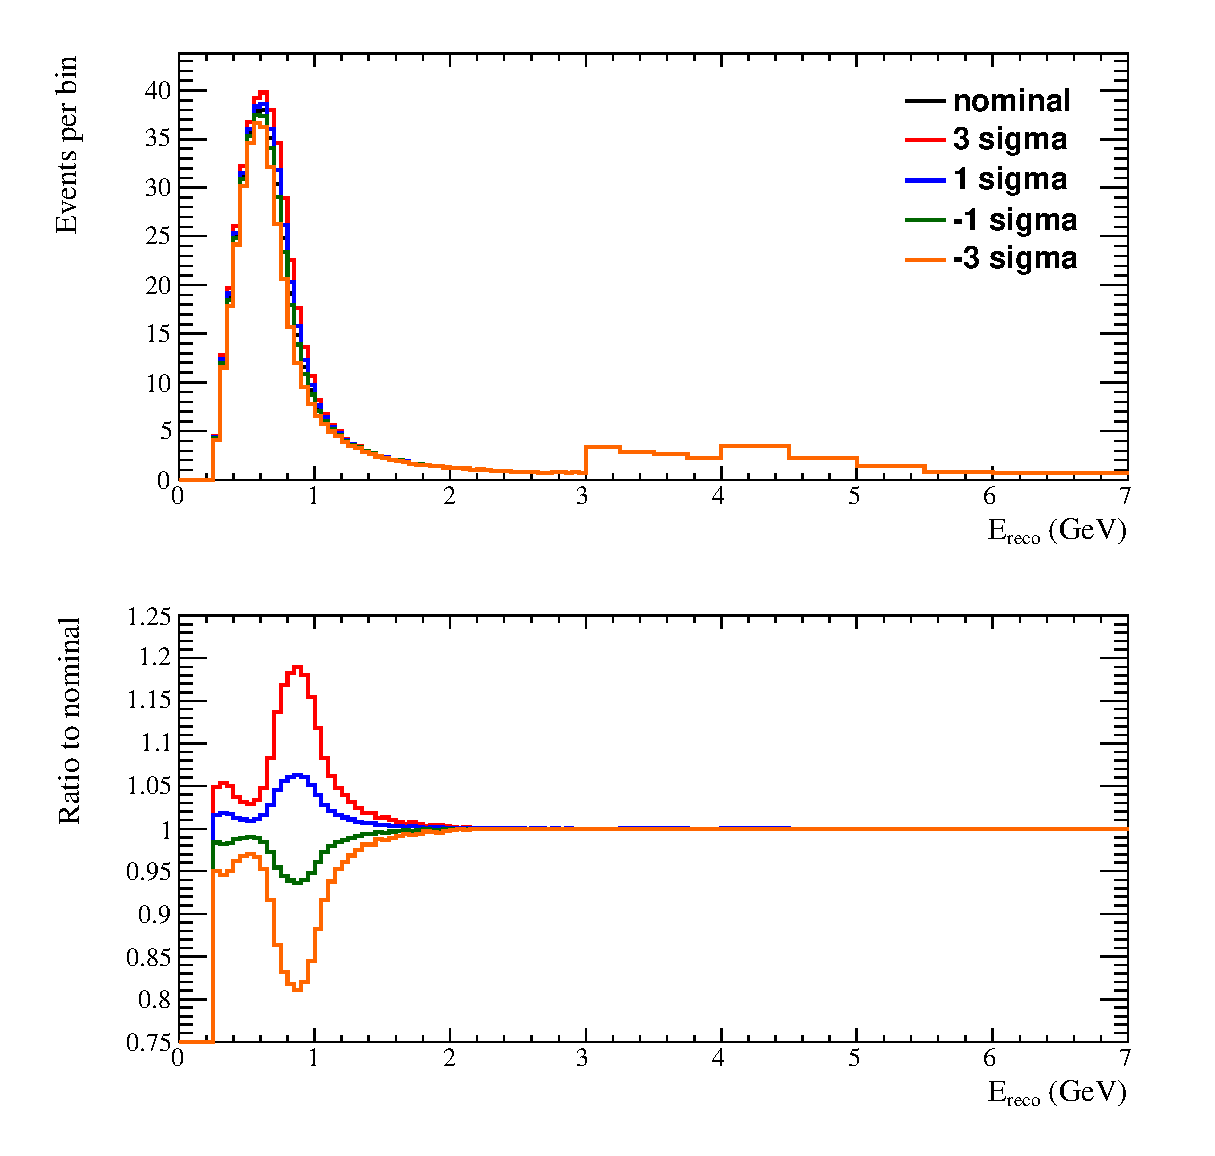
\includegraphics{../images/spectrum_tweaked/1sigma_unoscillated/ereco_twk_f_banff04}}
\caption
{ Effect of $f_{4; t, r}^{banff}$ for no oscillations (all mixing angles set to 0). }
\label{fig:noosc_ereco_twk_f_banff04}
\end{center}
\end{figure}
\clearpage

\begin{figure}
\begin{center}
\resizebox{14cm}{!}{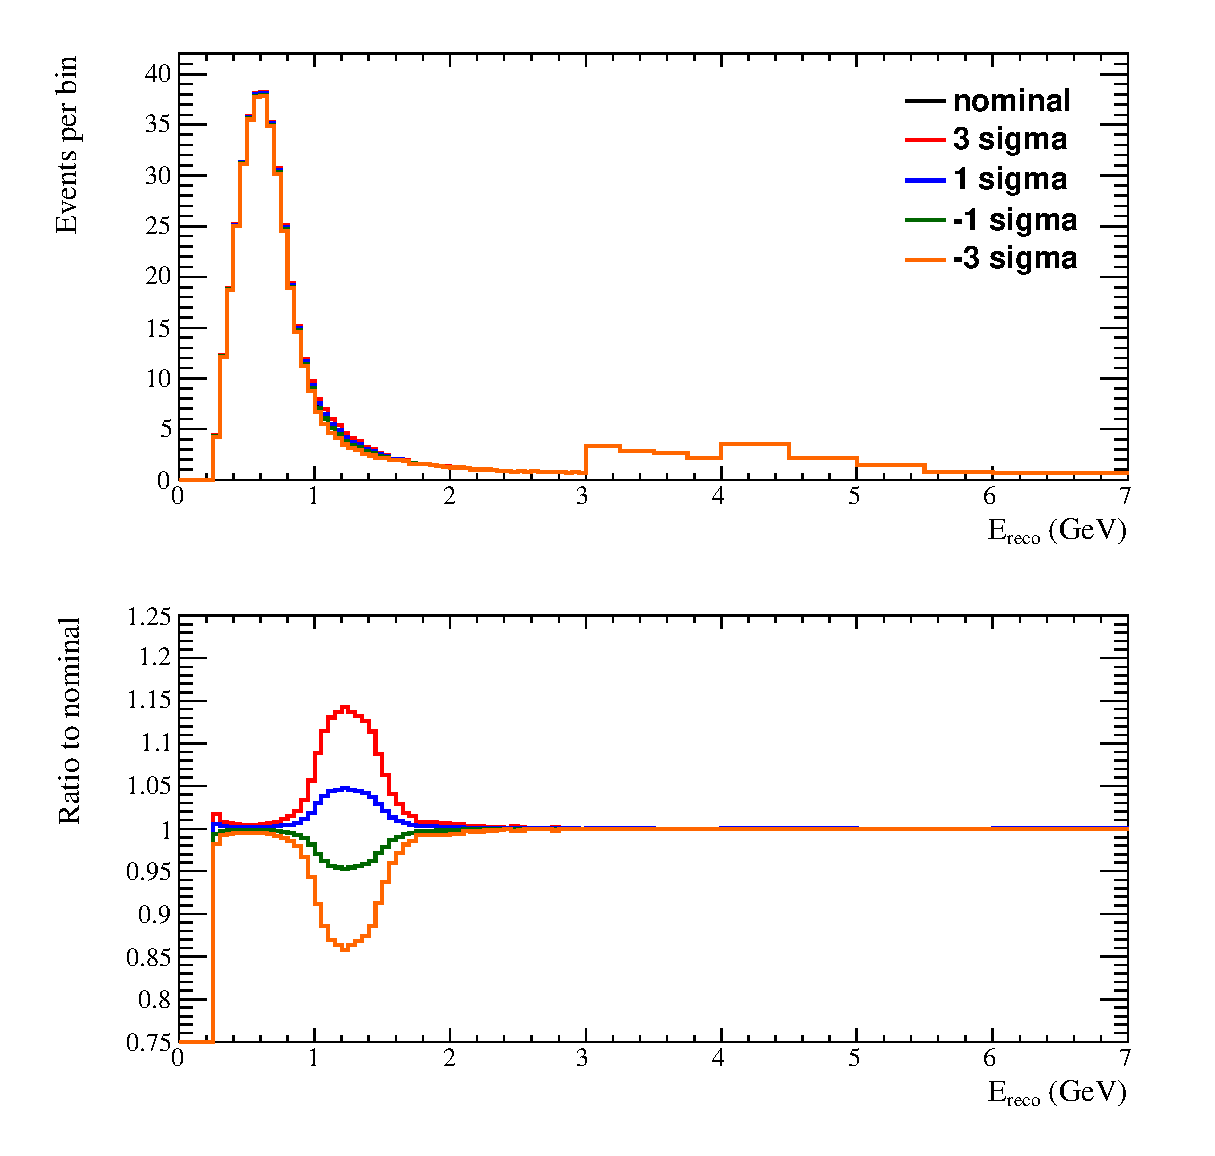
\includegraphics{../images/spectrum_tweaked/1sigma_unoscillated/ereco_twk_f_banff05}}
\caption
{ Effect of $f_{5; t, r}^{banff}$ for no oscillations (all mixing angles set to 0). }
\label{fig:noosc_ereco_twk_f_banff05}
\end{center}
\end{figure}
\clearpage

\begin{figure}
\begin{center}
\resizebox{14cm}{!}{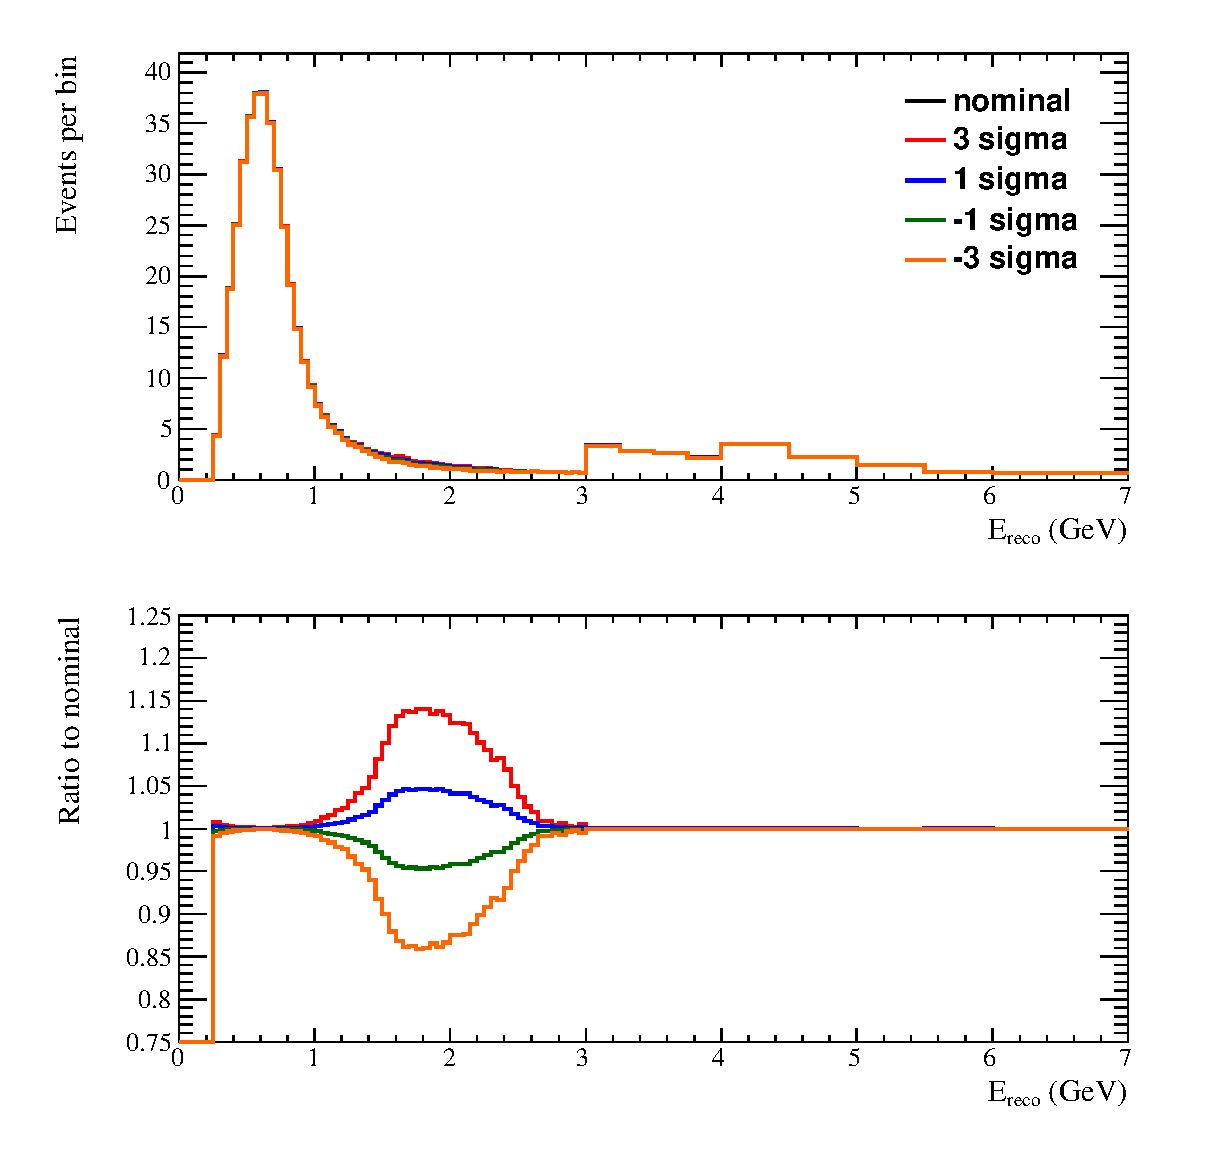
\includegraphics{../images/spectrum_tweaked/1sigma_unoscillated/ereco_twk_f_banff06}}
\caption
{ Effect of $f_{6; t, r}^{banff}$ for no oscillations (all mixing angles set to 0). }
\label{fig:noosc_ereco_twk_f_banff06}
\end{center}
\end{figure}
\clearpage

\begin{figure}
\begin{center}
\resizebox{14cm}{!}{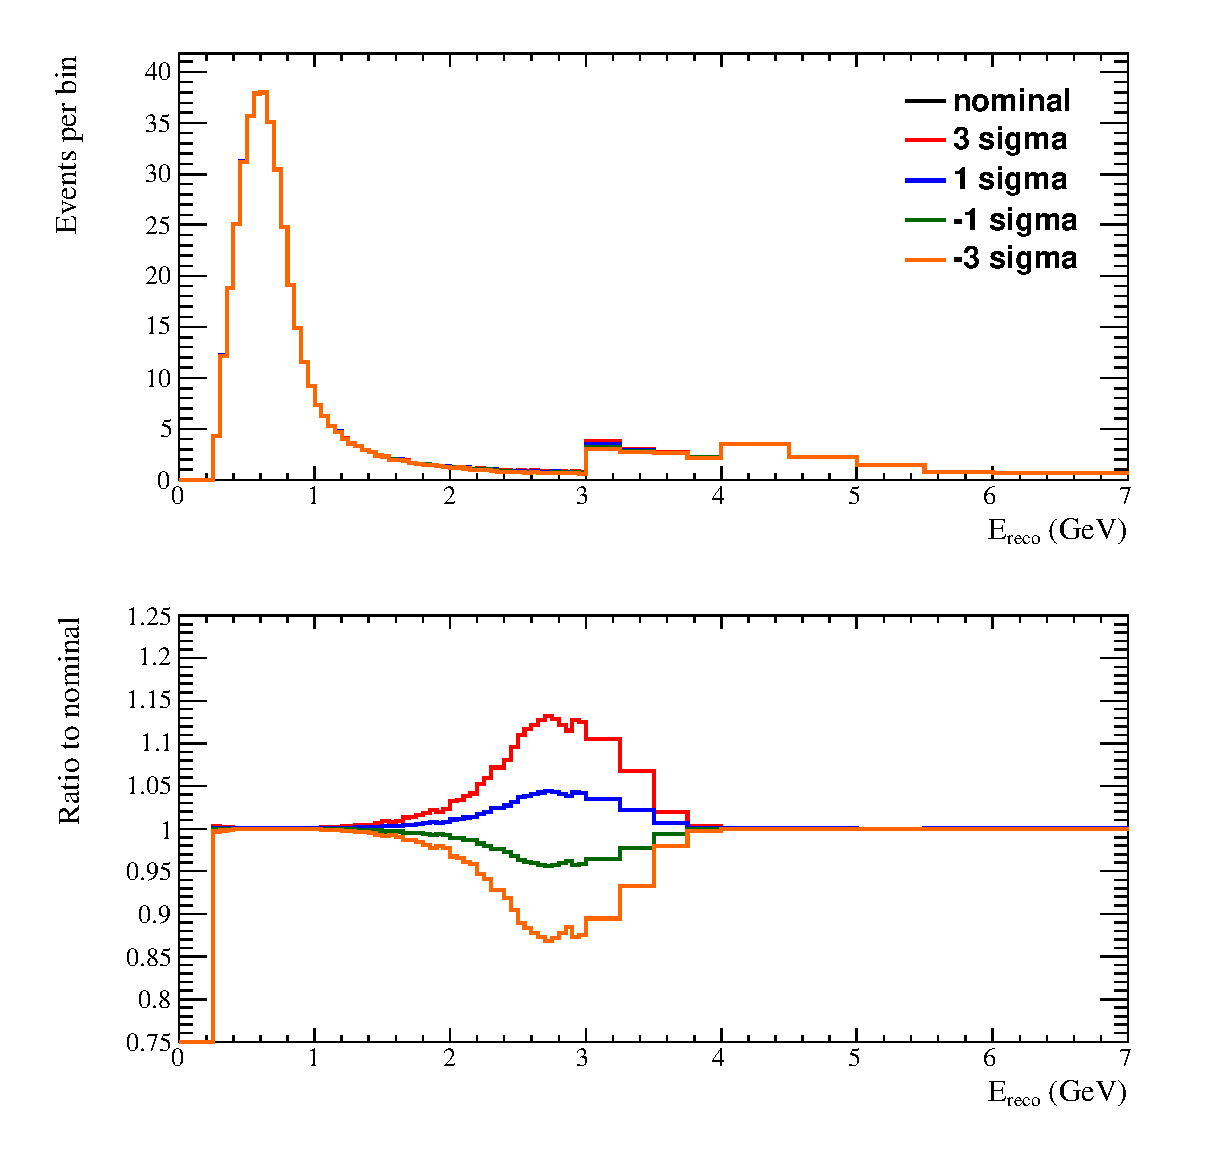
\includegraphics{../images/spectrum_tweaked/1sigma_unoscillated/ereco_twk_f_banff07}}
\caption
{ Effect of $f_{7; t, r}^{banff}$ for no oscillations (all mixing angles set to 0). }
\label{fig:noosc_ereco_twk_f_banff07}
\end{center}
\end{figure}
\clearpage

\begin{figure}
\begin{center}
\resizebox{14cm}{!}{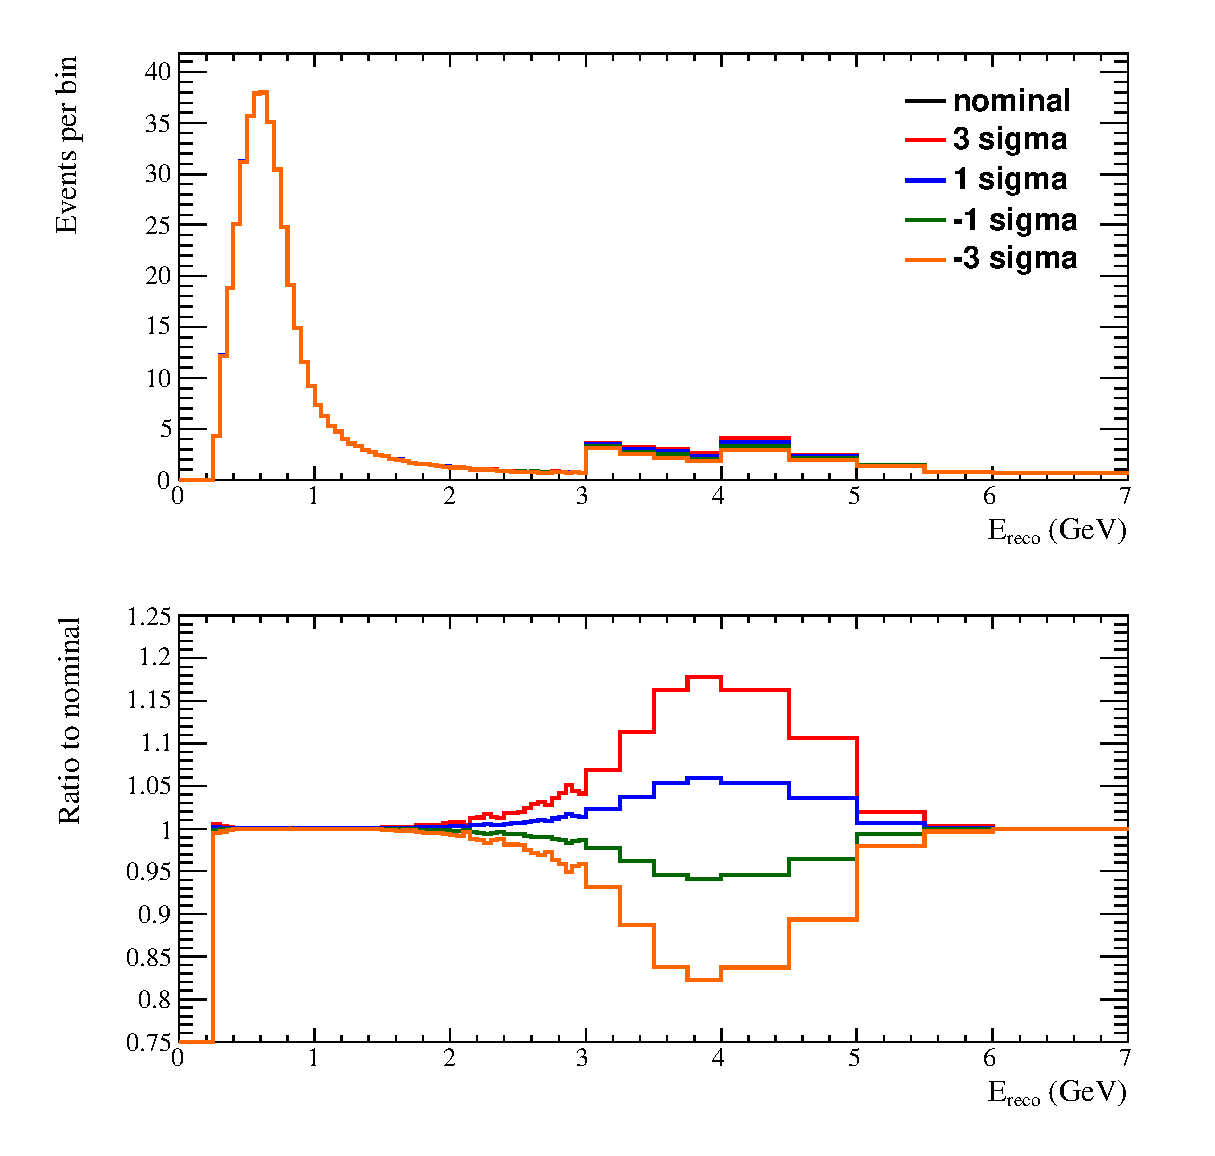
\includegraphics{../images/spectrum_tweaked/1sigma_unoscillated/ereco_twk_f_banff08}}
\caption
{ Effect of $f_{8; t, r}^{banff}$ for no oscillations (all mixing angles set to 0). }
\label{fig:noosc_ereco_twk_f_banff08}
\end{center}
\end{figure}
\clearpage

\begin{figure}
\begin{center}
\resizebox{14cm}{!}{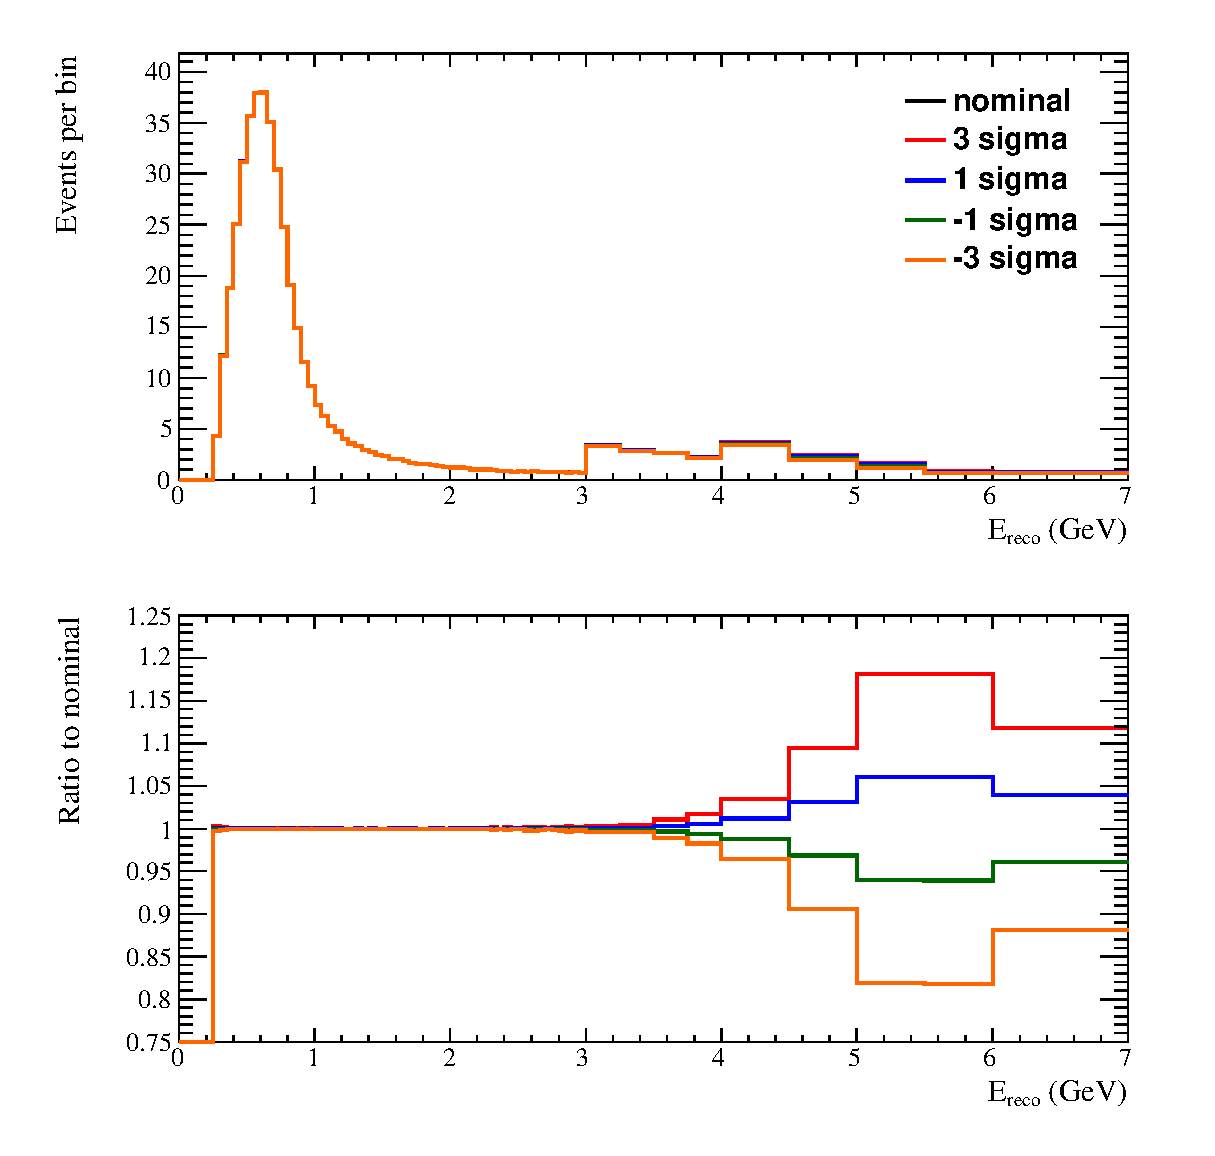
\includegraphics{../images/spectrum_tweaked/1sigma_unoscillated/ereco_twk_f_banff09}}
\caption
{ Effect of $f_{9; t, r}^{banff}$ for no oscillations (all mixing angles set to 0). }
\label{fig:noosc_ereco_twk_f_banff09}
\end{center}
\end{figure}
\clearpage

\begin{figure}
\begin{center}
\resizebox{14cm}{!}{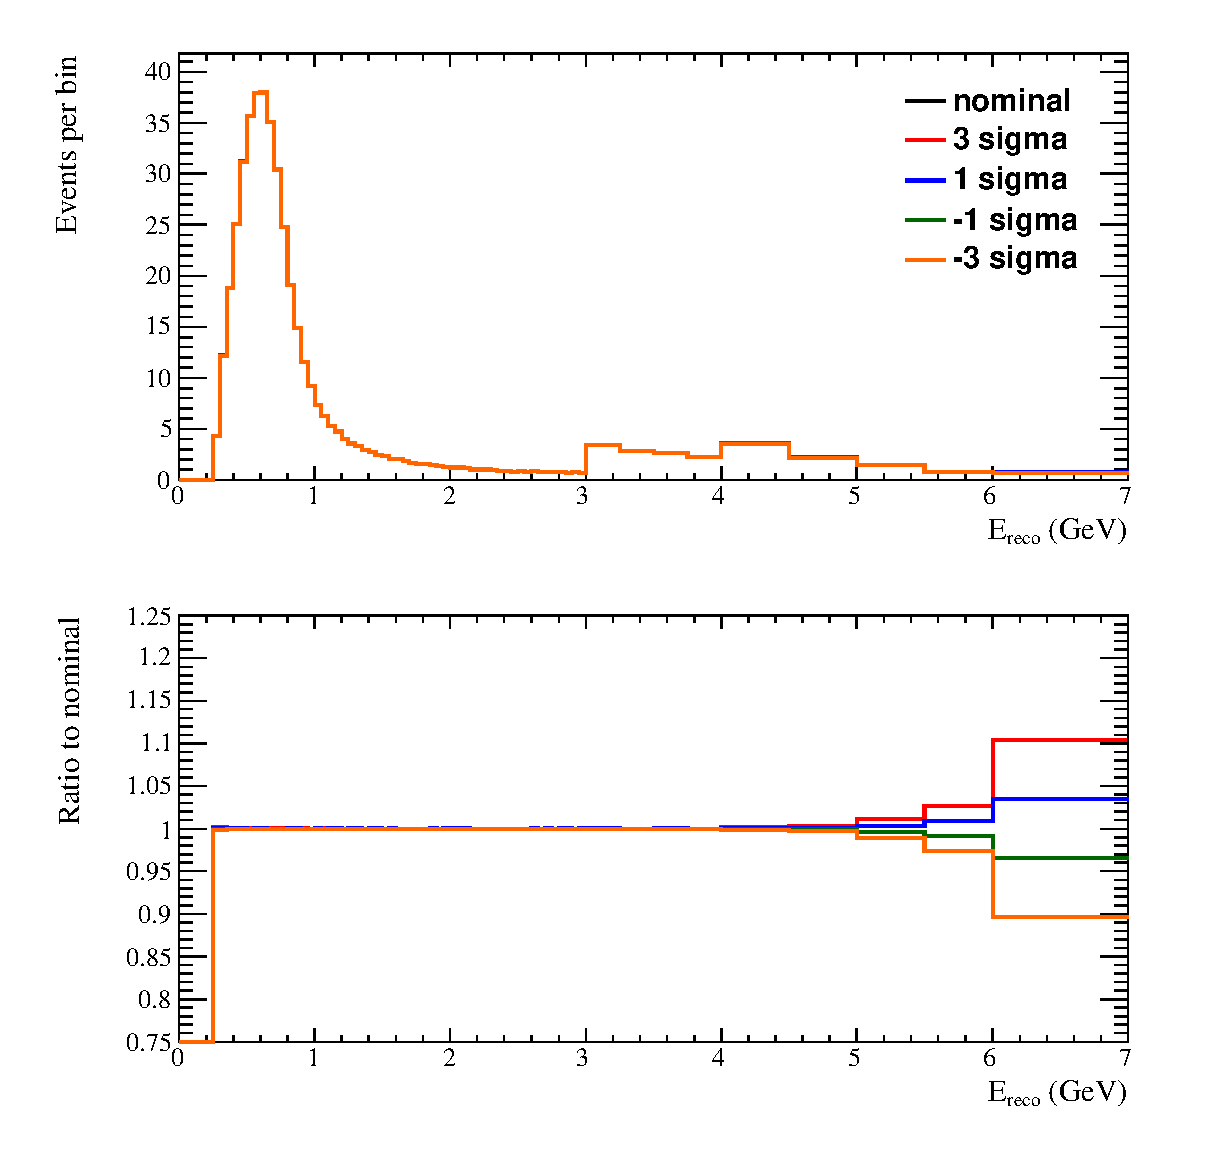
\includegraphics{../images/spectrum_tweaked/1sigma_unoscillated/ereco_twk_f_banff10}}
\caption
{ Effect of $f_{10; t, r}^{banff}$ for no oscillations (all mixing angles set to 0). }
\label{fig:noosc_ereco_twk_f_banff10}
\end{center}
\end{figure}
\clearpage

\begin{figure}
\begin{center}
\resizebox{14cm}{!}{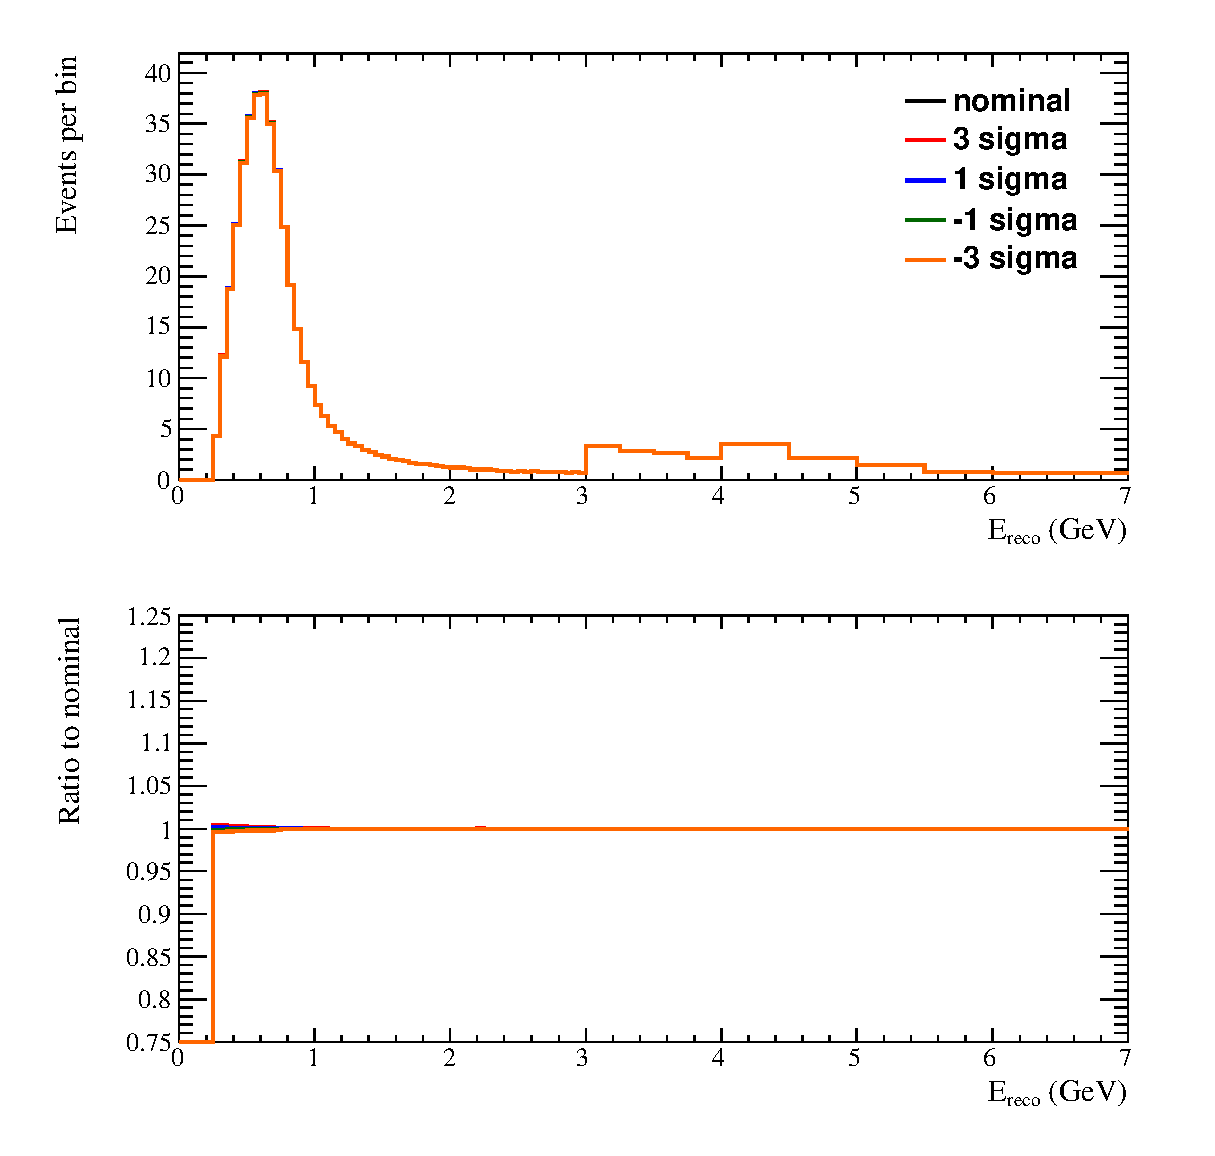
\includegraphics{../images/spectrum_tweaked/1sigma_unoscillated/ereco_twk_f_banff11}}
\caption
{ Effect of $f_{11; t, r}^{banff}$ for no oscillations (all mixing angles set to 0). }
\label{fig:noosc_ereco_twk_f_banff11}
\end{center}
\end{figure}
\clearpage

\begin{figure}
\begin{center}
\resizebox{14cm}{!}{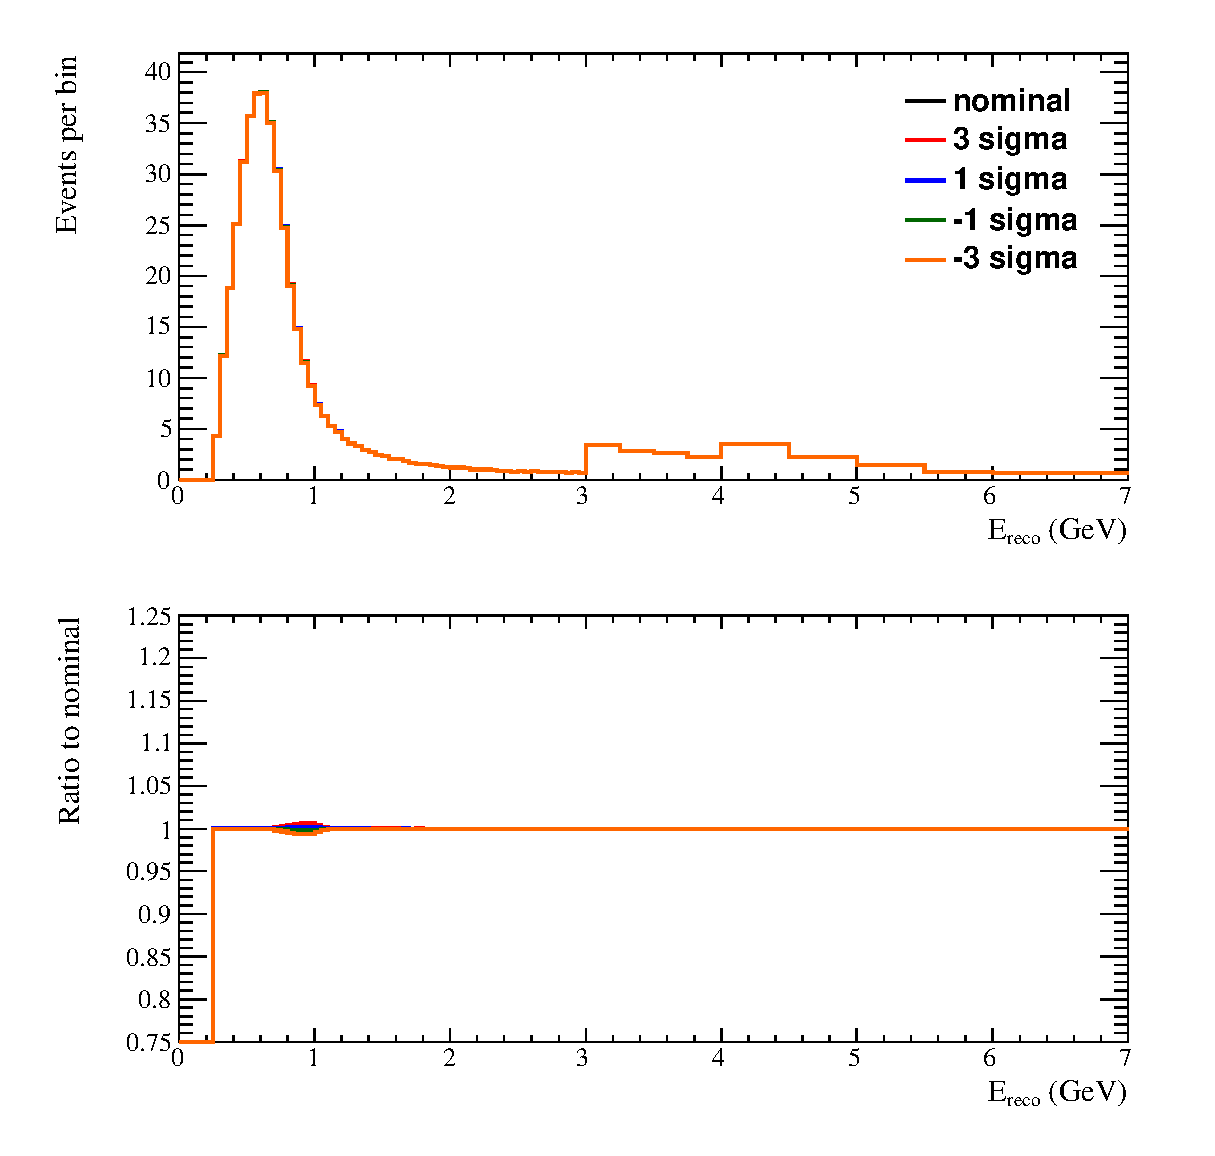
\includegraphics{../images/spectrum_tweaked/1sigma_unoscillated/ereco_twk_f_banff12}}
\caption
{ Effect of $f_{12; t, r}^{banff}$ for no oscillations (all mixing angles set to 0). }
\label{fig:noosc_ereco_twk_f_banff12}
\end{center}
\end{figure}
\clearpage

\begin{figure}
\begin{center}
\resizebox{14cm}{!}{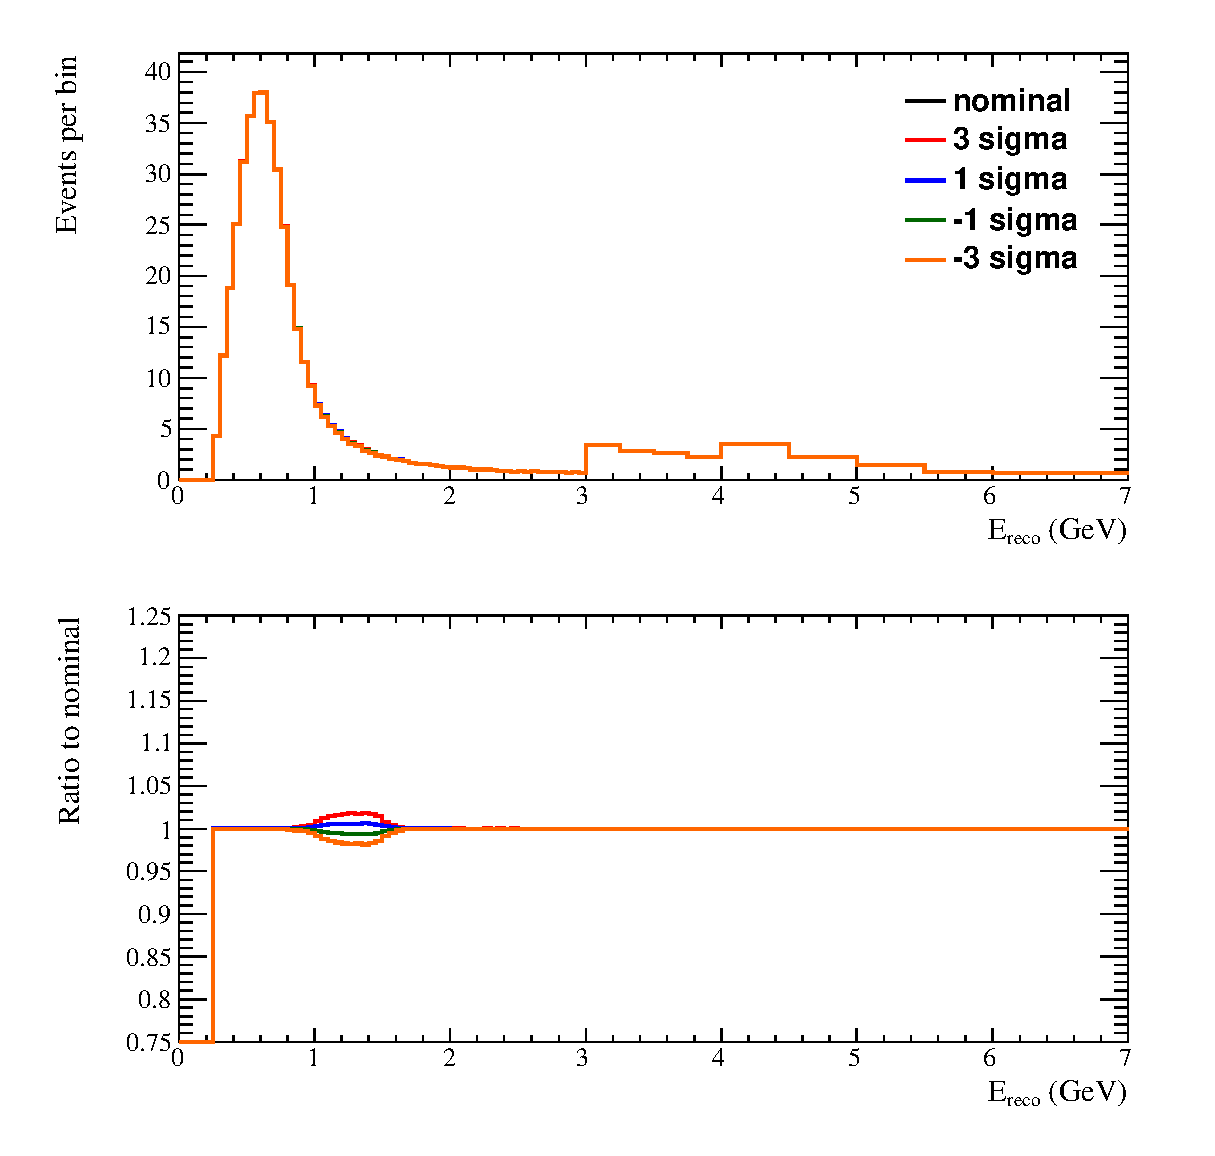
\includegraphics{../images/spectrum_tweaked/1sigma_unoscillated/ereco_twk_f_banff13}}
\caption
{ Effect of $f_{13; t, r}^{banff}$ for no oscillations (all mixing angles set to 0). }
\label{fig:noosc_ereco_twk_f_banff13}
\end{center}
\end{figure}
\clearpage

\begin{figure}
\begin{center}
\resizebox{14cm}{!}{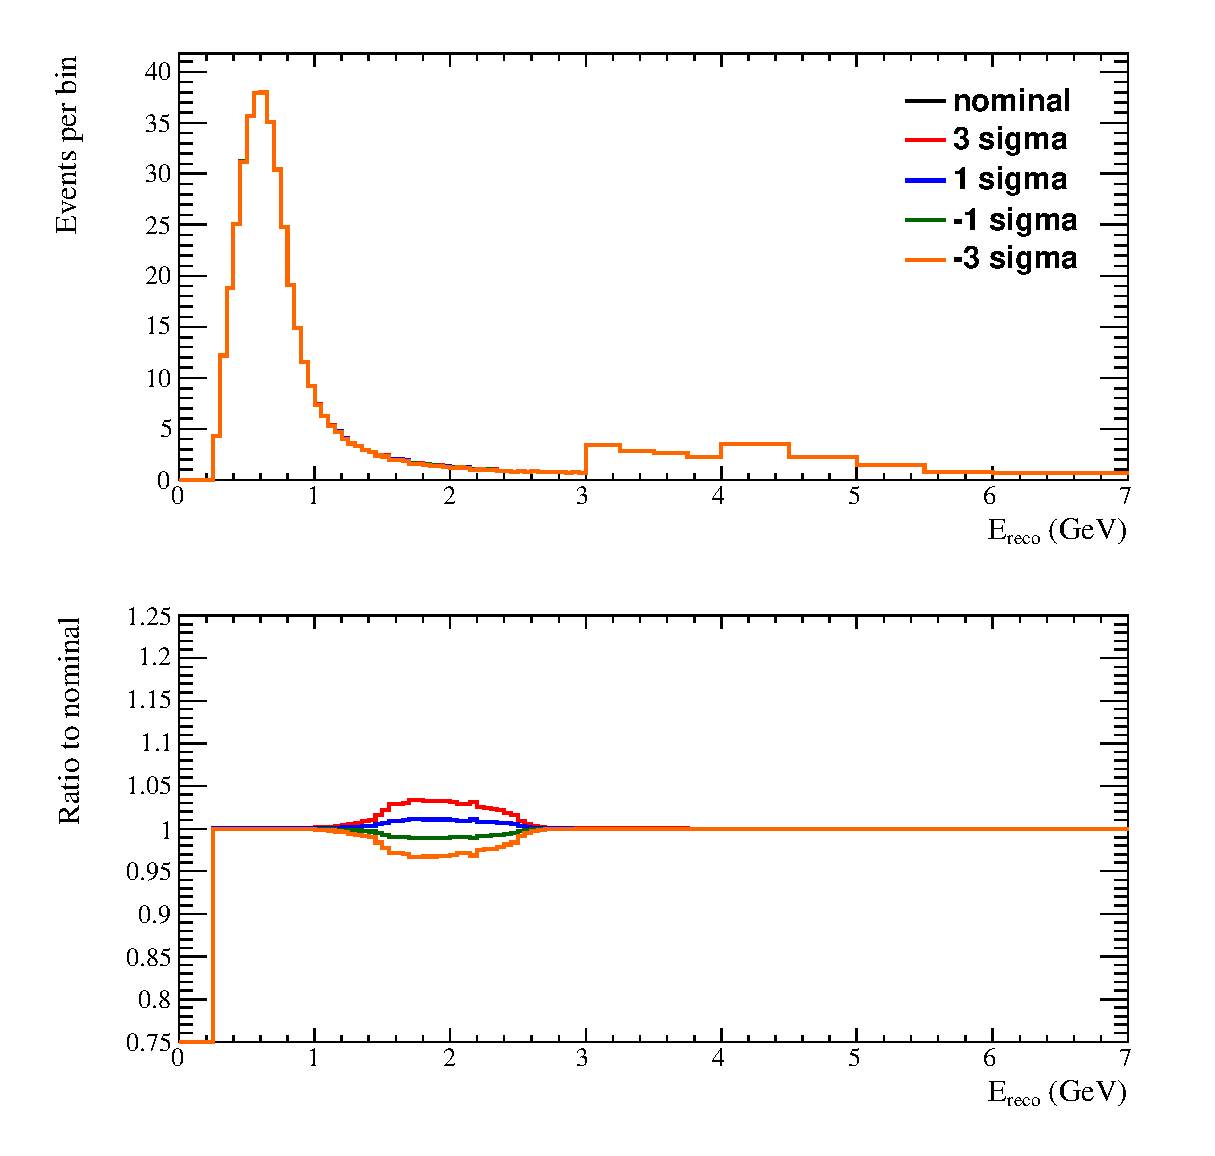
\includegraphics{../images/spectrum_tweaked/1sigma_unoscillated/ereco_twk_f_banff14}}
\caption
{ Effect of $f_{14; t, r}^{banff}$ for no oscillations (all mixing angles set to 0). }
\label{fig:noosc_ereco_twk_f_banff14}
\end{center}
\end{figure}
\clearpage

\begin{figure}
\begin{center}
\resizebox{14cm}{!}{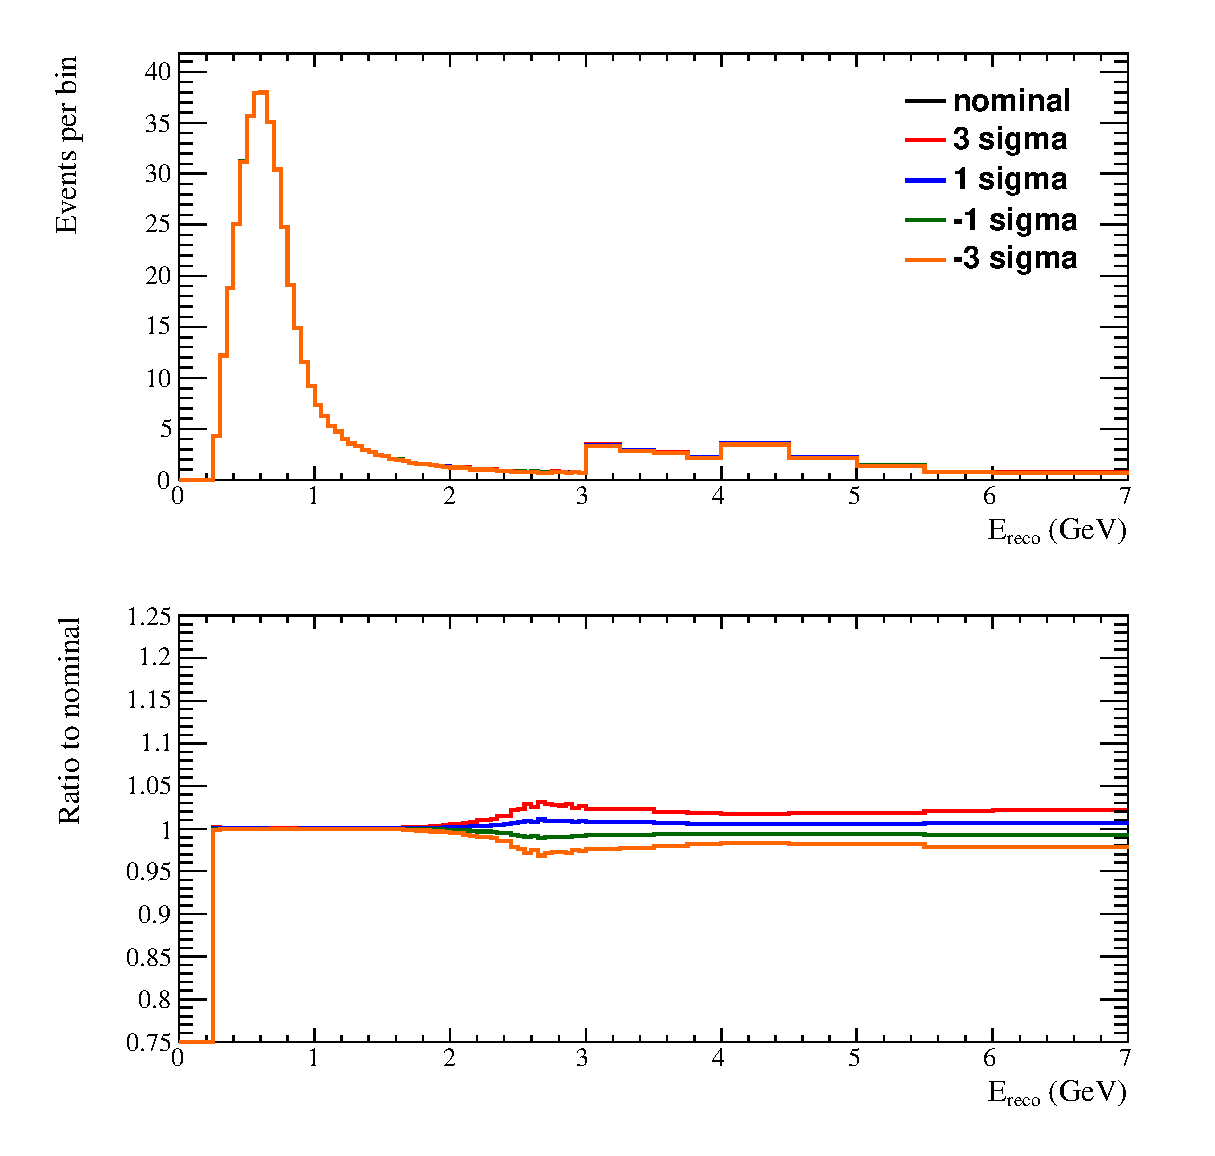
\includegraphics{../images/spectrum_tweaked/1sigma_unoscillated/ereco_twk_f_banff15}}
\caption
{ Effect of $f_{15; t, r}^{banff}$ for no oscillations (all mixing angles set to 0). }
\label{fig:noosc_ereco_twk_f_banff15}
\end{center}
\end{figure}
\clearpage

\begin{figure}
\begin{center}
\resizebox{14cm}{!}{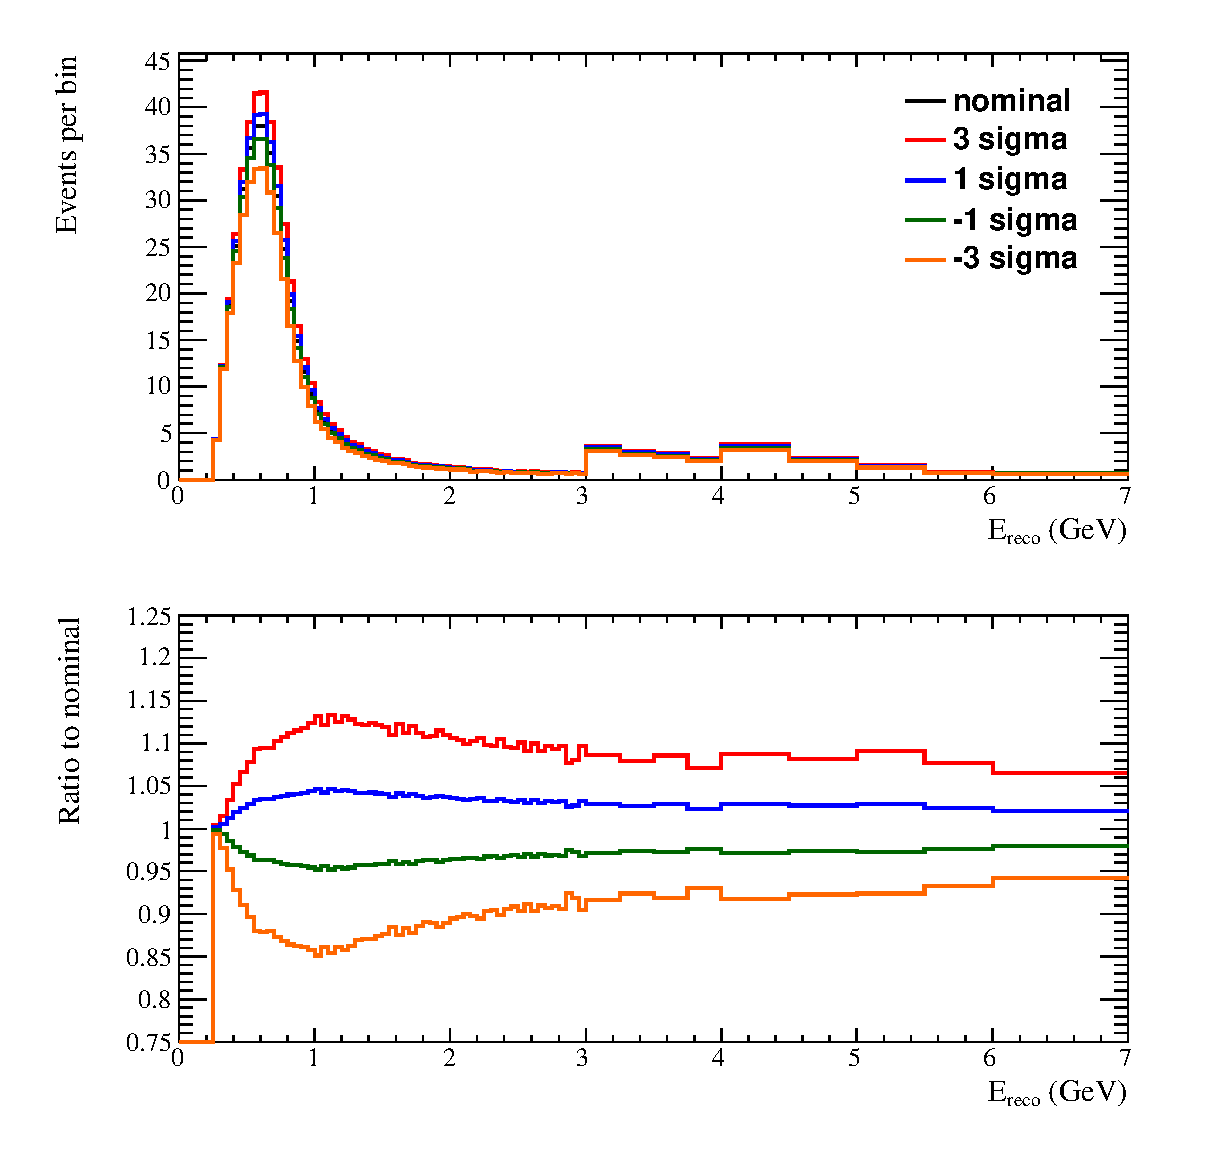
\includegraphics{../images/spectrum_tweaked/1sigma_unoscillated/ereco_twk_f_banffmaqe}}
\caption
{ Effect of $f_{16; t, r}^{banff}$ for no oscillations (all mixing angles set to 0). }
\label{fig:noosc_ereco_twk_f_banffmaqe}
\end{center}
\end{figure}
\clearpage

\begin{figure}
\begin{center}
\resizebox{14cm}{!}{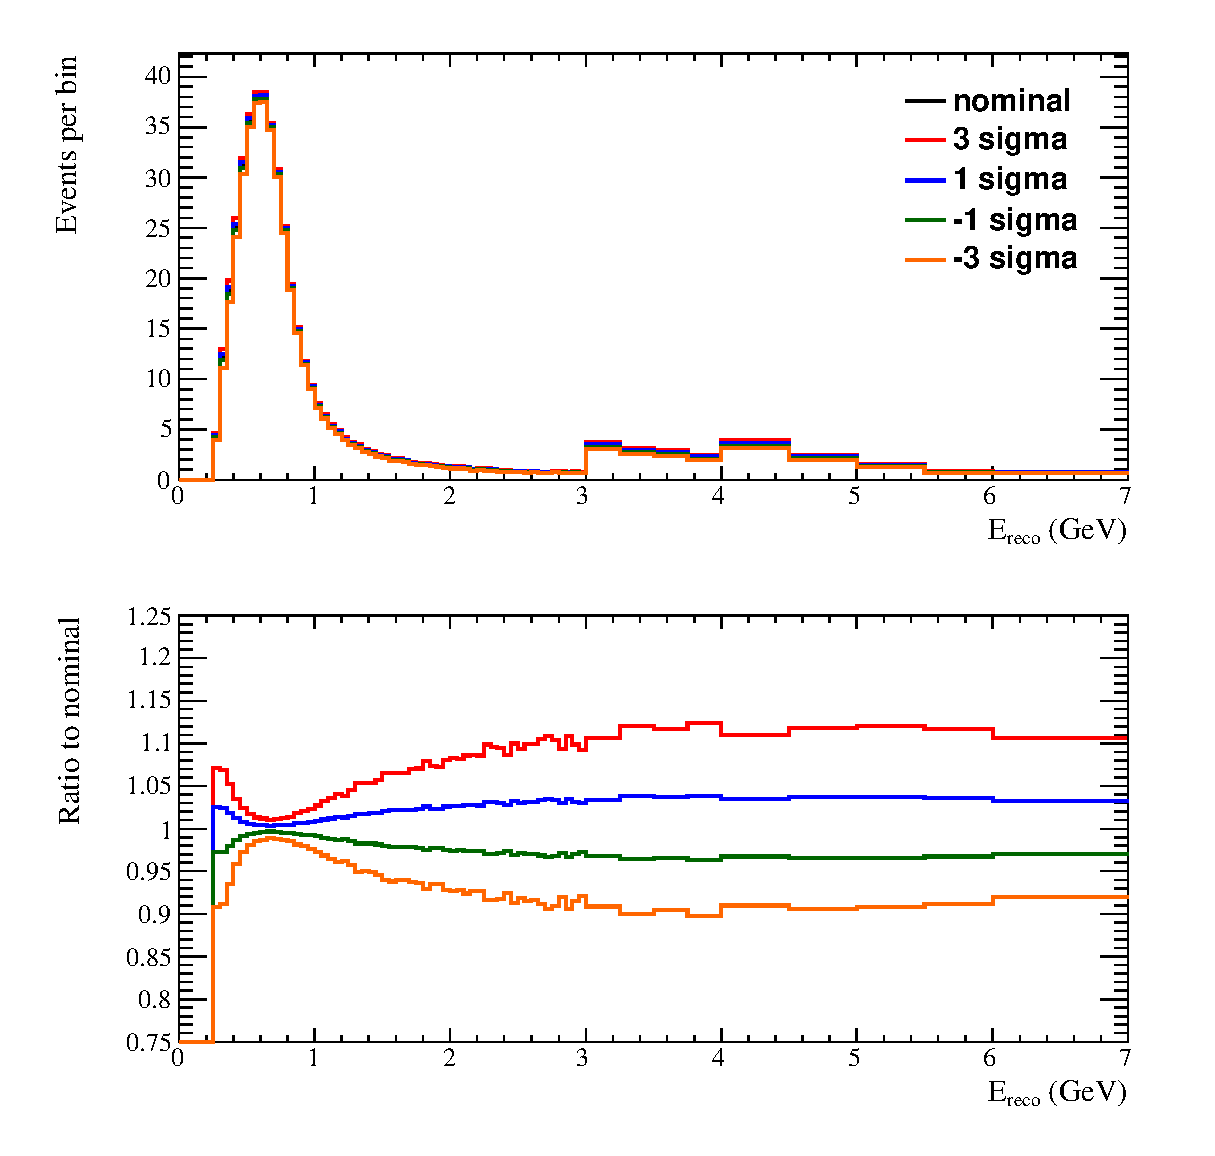
\includegraphics{../images/spectrum_tweaked/1sigma_unoscillated/ereco_twk_f_banffmares}}
\caption
{ Effect of $f_{17; t, r}^{banff}$ for no oscillations (all mixing angles set to 0). }
\label{fig:noosc_ereco_twk_f_banffmares}
\end{center}
\end{figure}
\clearpage

\begin{figure}
\begin{center}
\resizebox{14cm}{!}{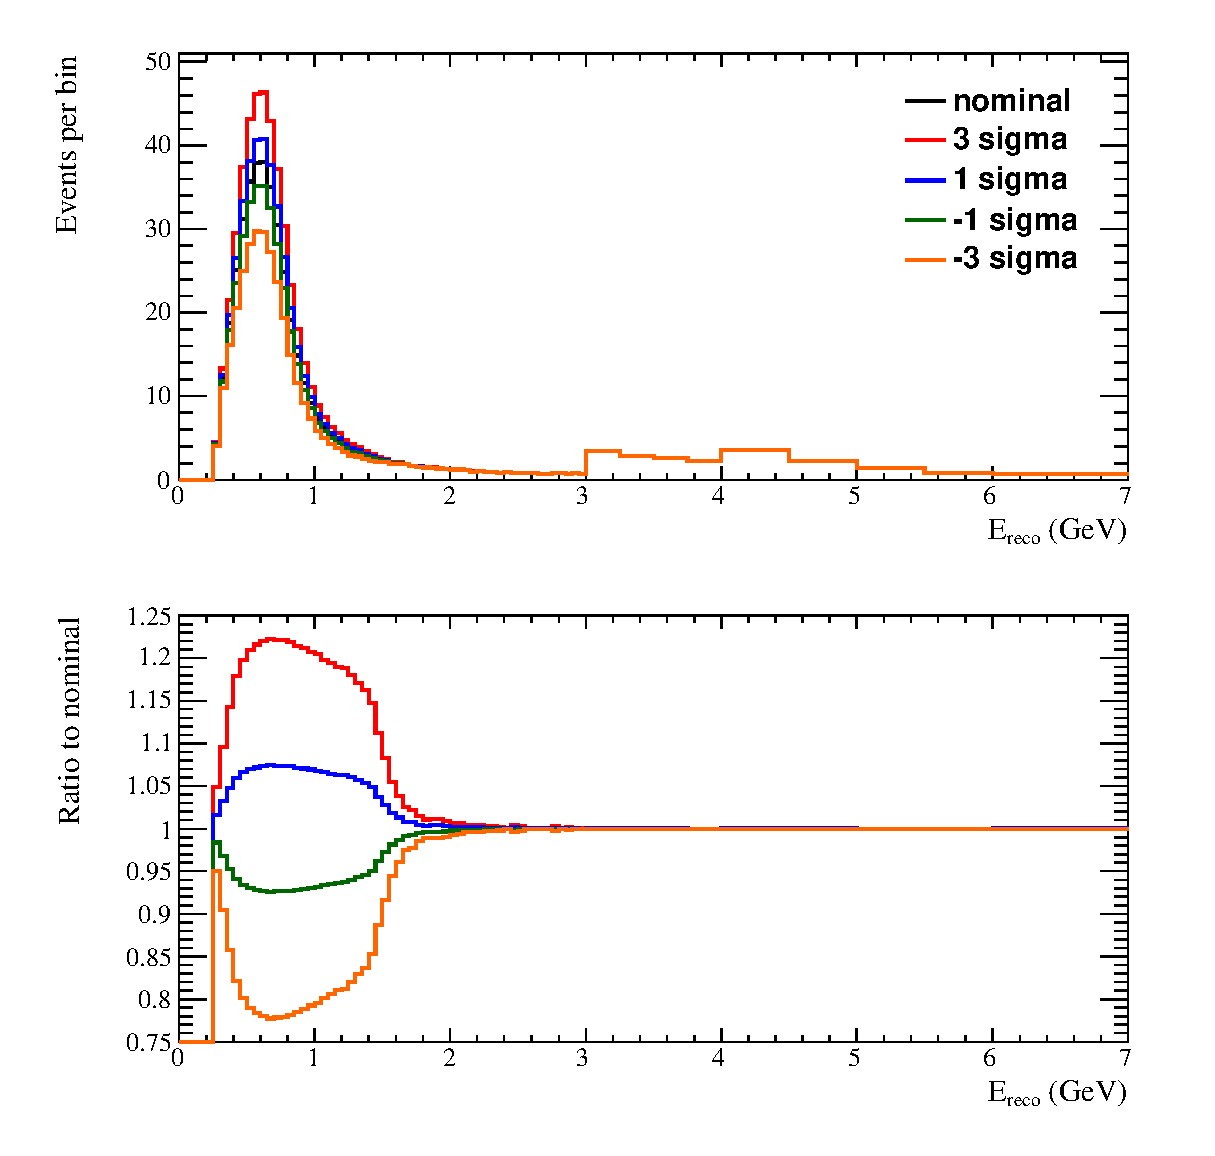
\includegraphics{../images/spectrum_tweaked/1sigma_unoscillated/ereco_twk_f_banffccqee0}}
\caption
{ Effect of $f_{18; t, r}^{banff}$ for no oscillations (all mixing angles set to 0). }
\label{fig:noosc_ereco_twk_f_banffccqee0}
\end{center}
\end{figure}
\clearpage

\begin{figure}
\begin{center}
\resizebox{14cm}{!}{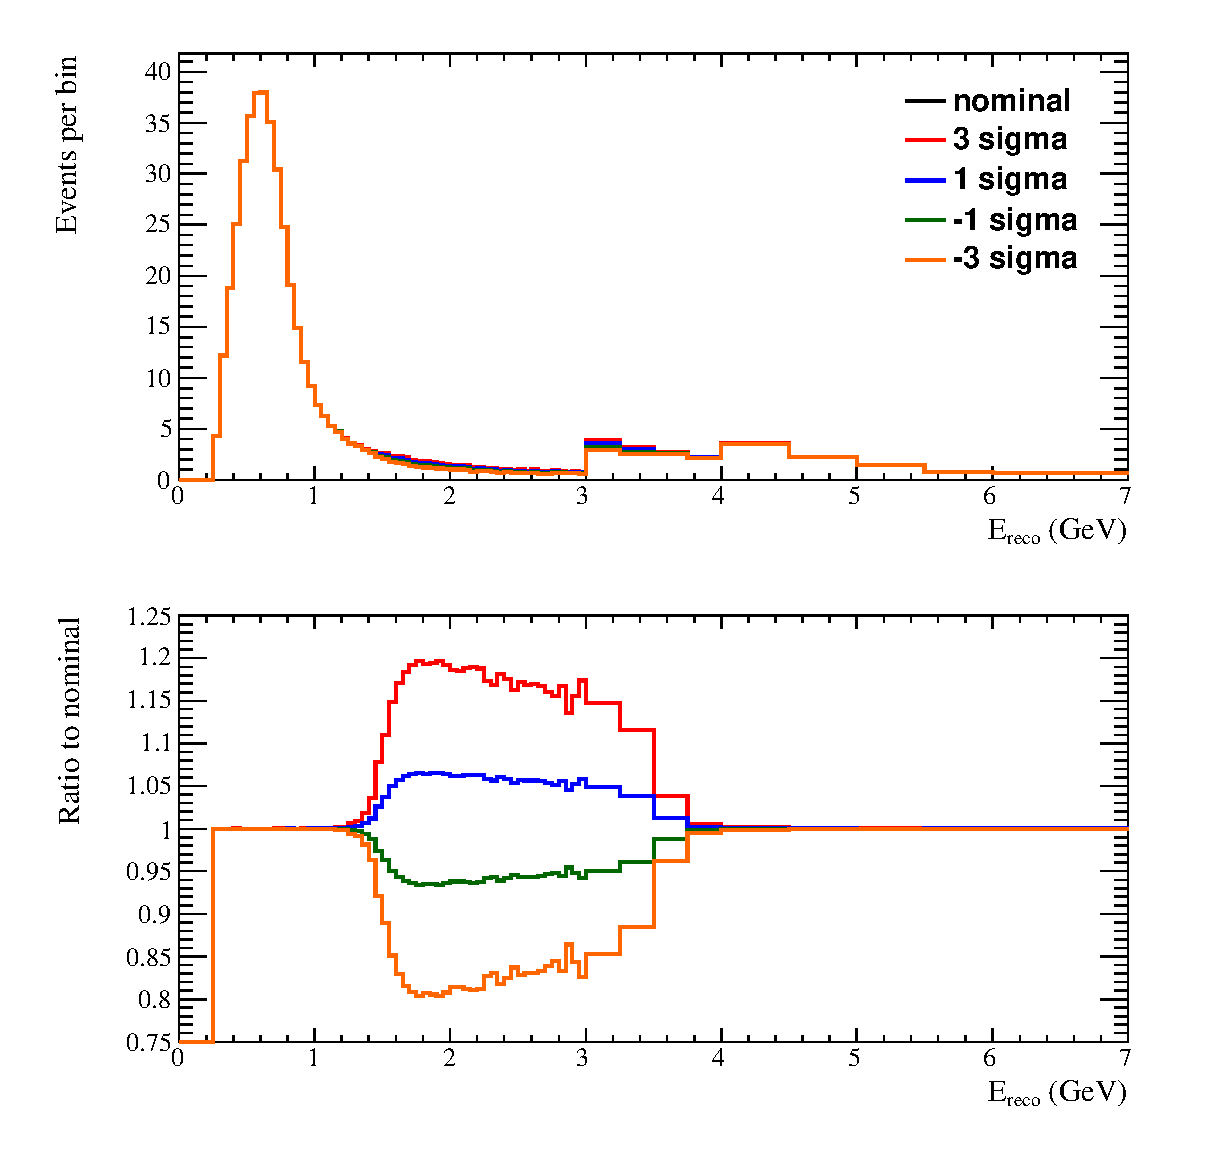
\includegraphics{../images/spectrum_tweaked/1sigma_unoscillated/ereco_twk_f_banffccqee1}}
\caption
{ Effect of $f_{19; t, r}^{banff}$ for no oscillations (all mixing angles set to 0). }
\label{fig:noosc_ereco_twk_f_banffccqee1}
\end{center}
\end{figure}
\clearpage

\begin{figure}
\begin{center}
\resizebox{14cm}{!}{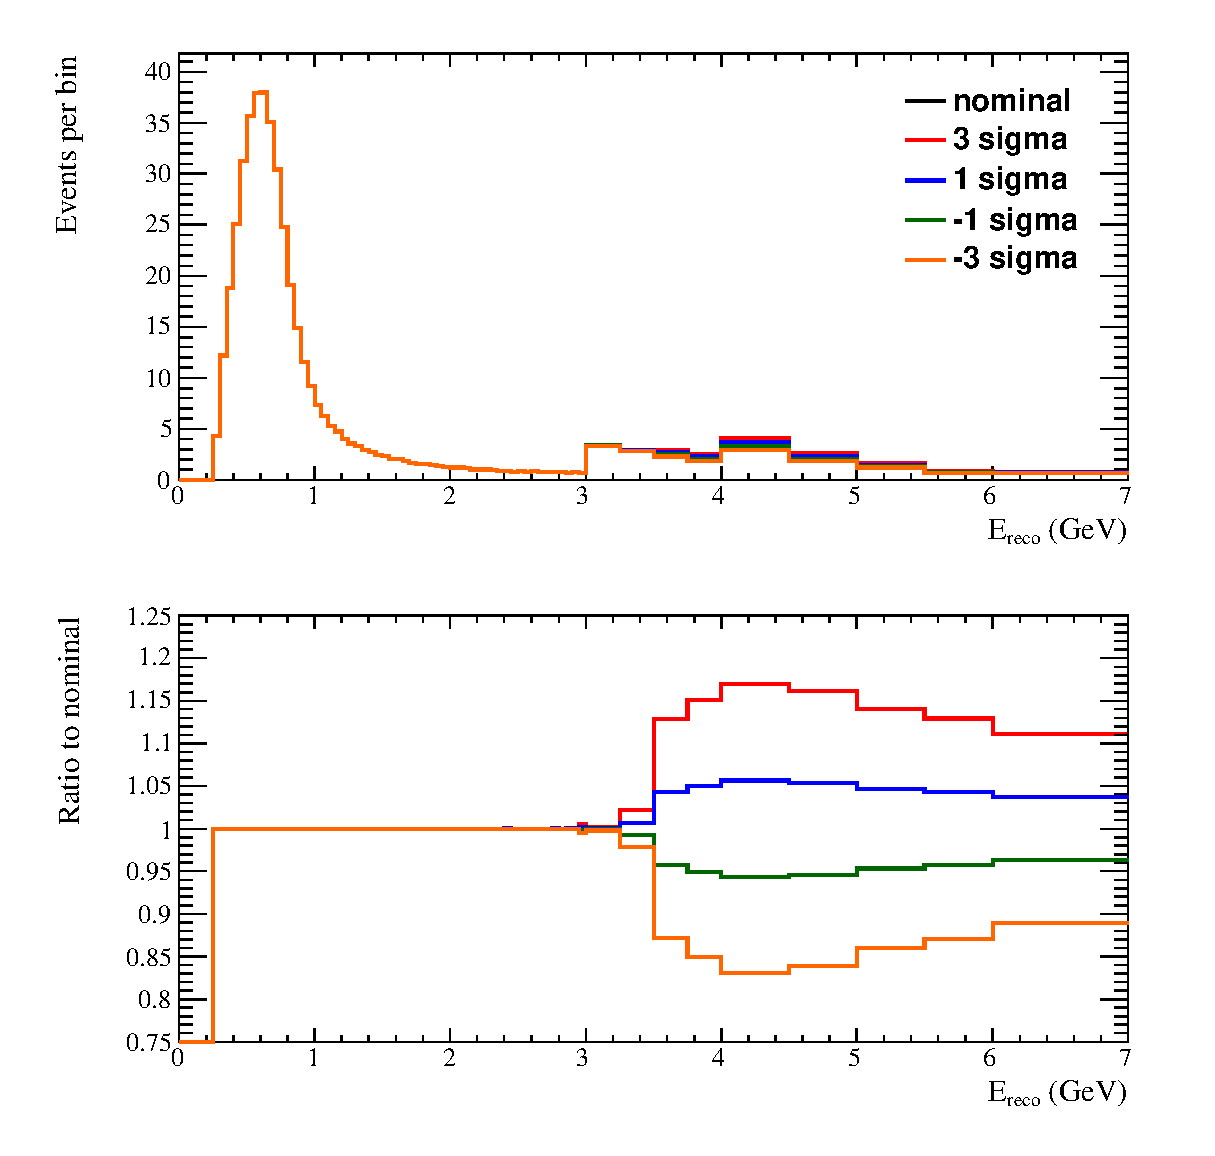
\includegraphics{../images/spectrum_tweaked/1sigma_unoscillated/ereco_twk_f_banffccqee2}}
\caption
{ Effect of $f_{20; t, r}^{banff}$ for no oscillations (all mixing angles set to 0). }
\label{fig:noosc_ereco_twk_f_banffccqee2}
\end{center}
\end{figure}
\clearpage

\begin{figure}
\begin{center}
\resizebox{14cm}{!}{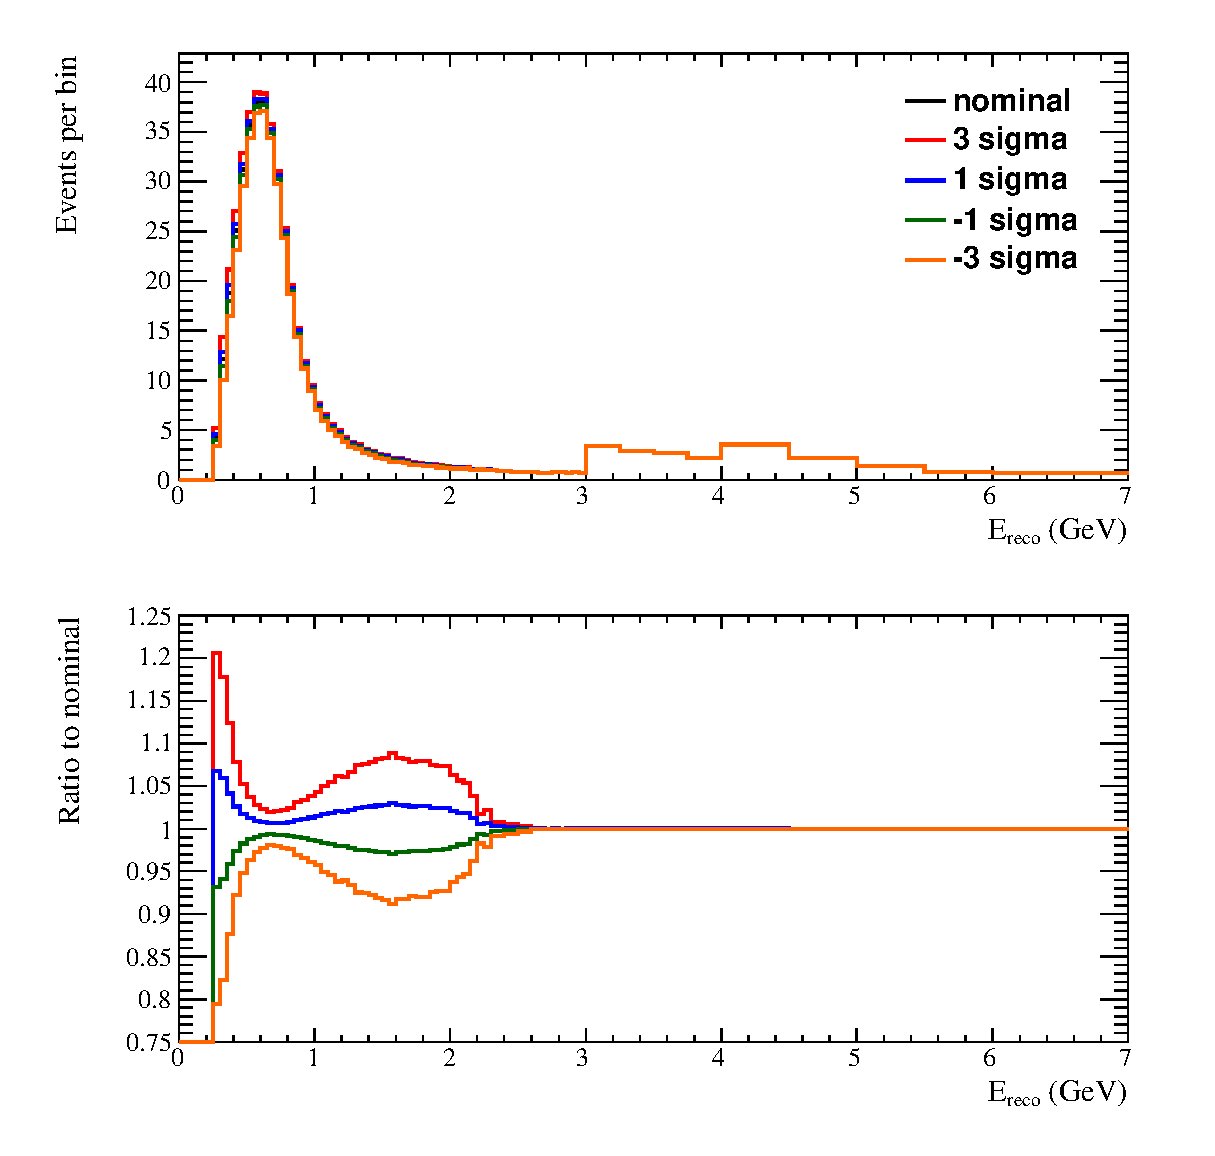
\includegraphics{../images/spectrum_tweaked/1sigma_unoscillated/ereco_twk_f_banffcc1pie0}}
\caption
{ Effect of $f_{21; t, r}^{banff}$ for no oscillations (all mixing angles set to 0). }
\label{fig:noosc_ereco_twk_f_banffcc1pie0}
\end{center}
\end{figure}
\clearpage

\begin{figure}
\begin{center}
\resizebox{14cm}{!}{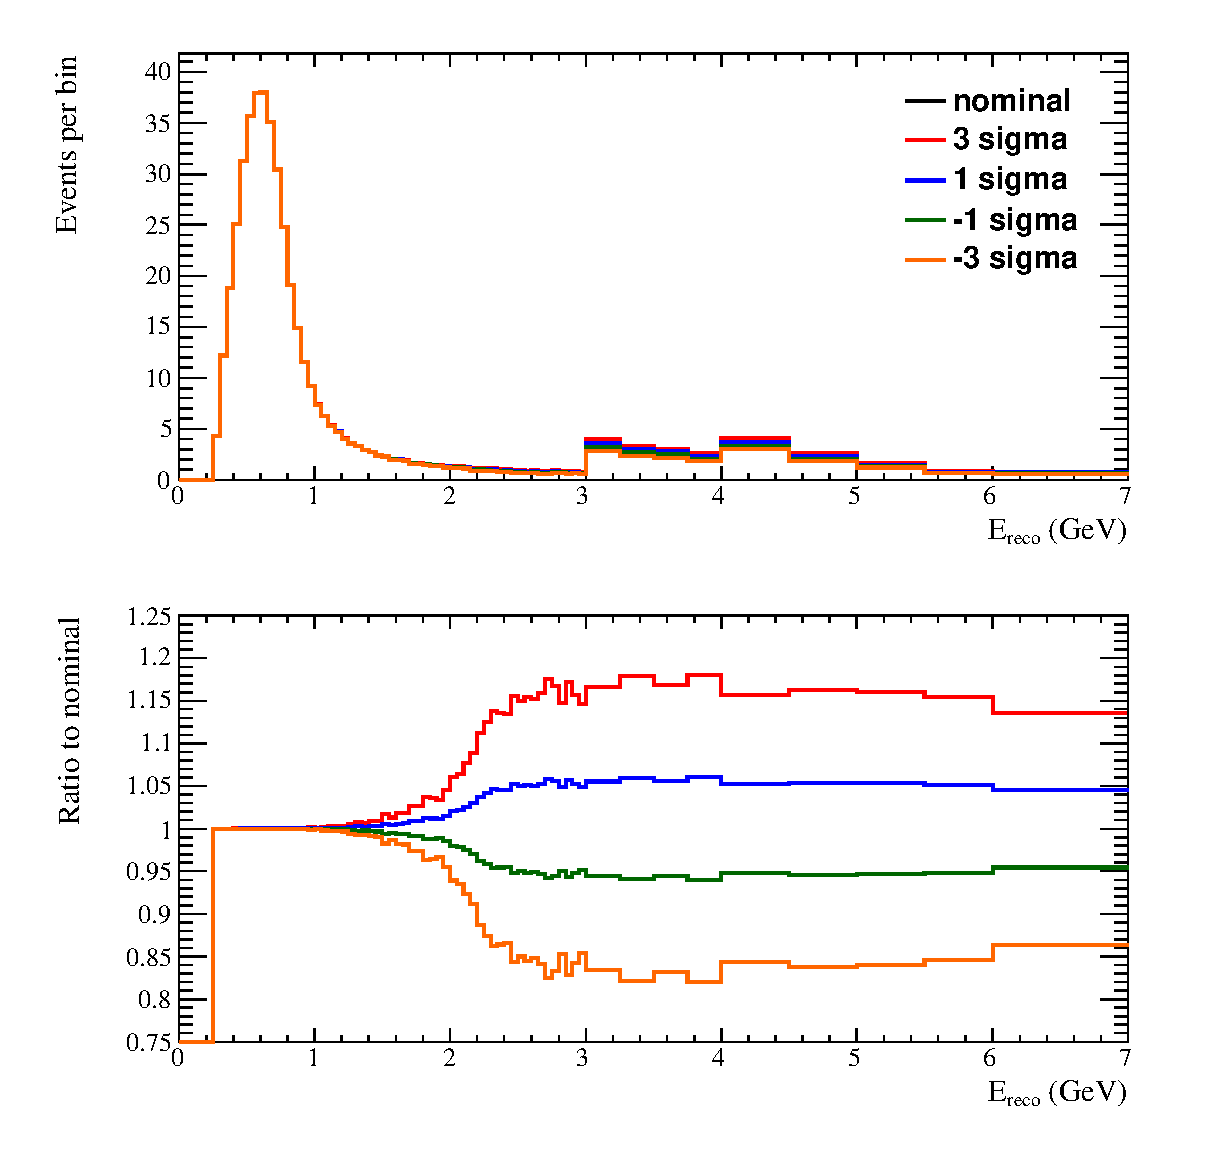
\includegraphics{../images/spectrum_tweaked/1sigma_unoscillated/ereco_twk_f_banffcc1pie1}}
\caption
{ Effect of $f_{22; t, r}^{banff}$ for no oscillations (all mixing angles set to 0). }
\label{fig:noosc_ereco_twk_f_banffcc1pie1}
\end{center}
\end{figure}
\clearpage

\begin{figure}
\begin{center}
\resizebox{14cm}{!}{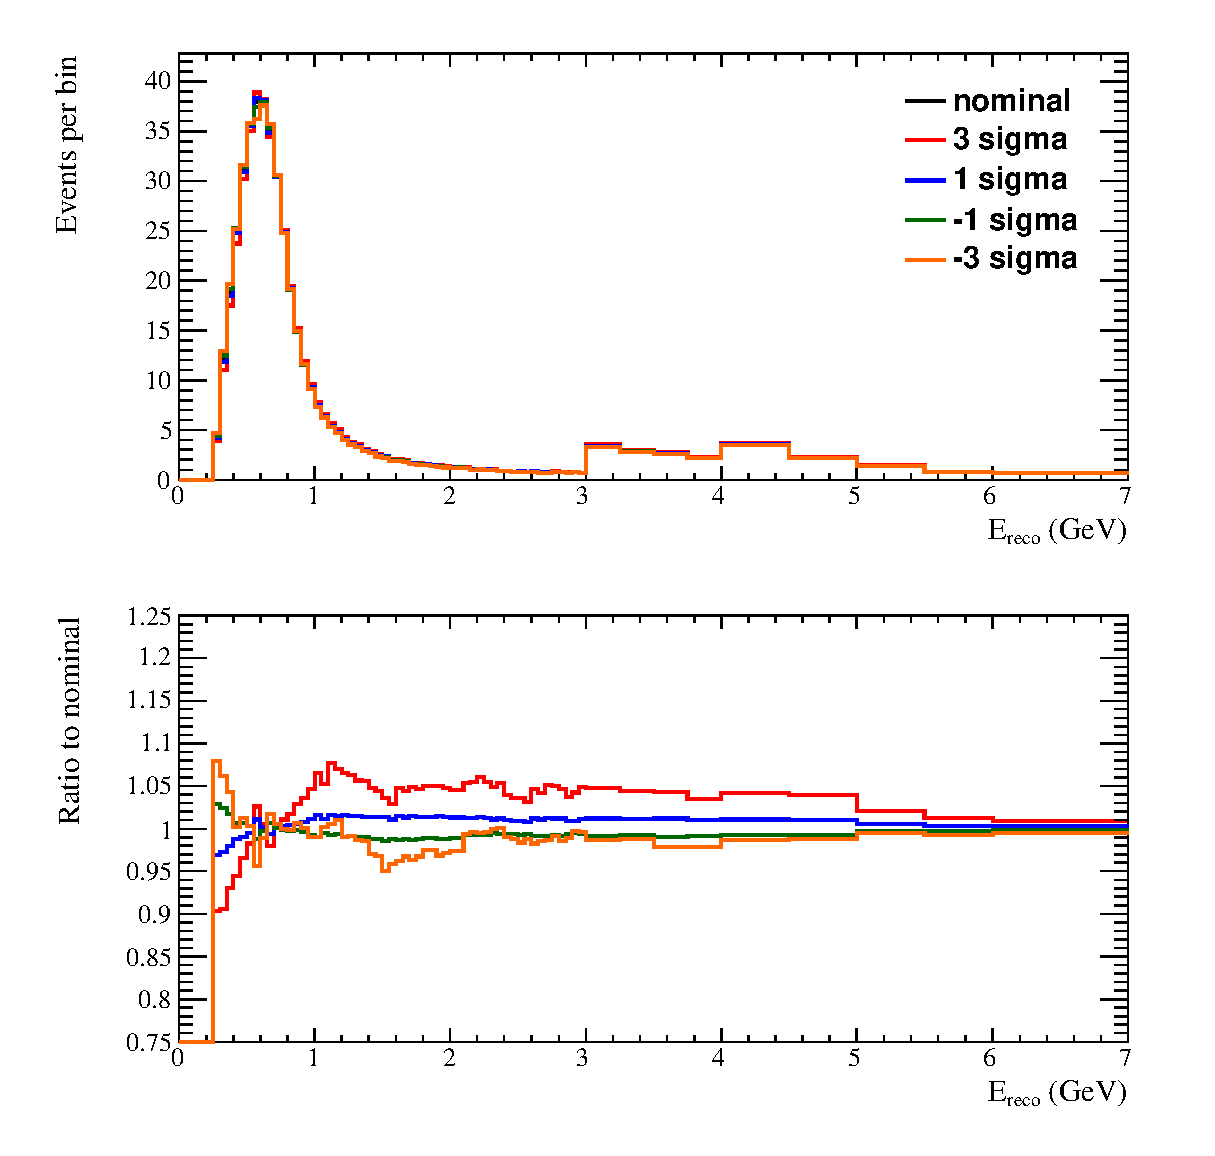
\includegraphics{../images/spectrum_tweaked/1sigma_unoscillated/ereco_twk_f_pfermi}}
\caption
{ Effect of $f_{pF; t, r}$ for no oscillations (all mixing angles set to 0). }
\label{fig:noosc_ereco_twk_f_pfermi}
\end{center}
\end{figure}
\clearpage

\begin{figure}
\begin{center}
\resizebox{14cm}{!}{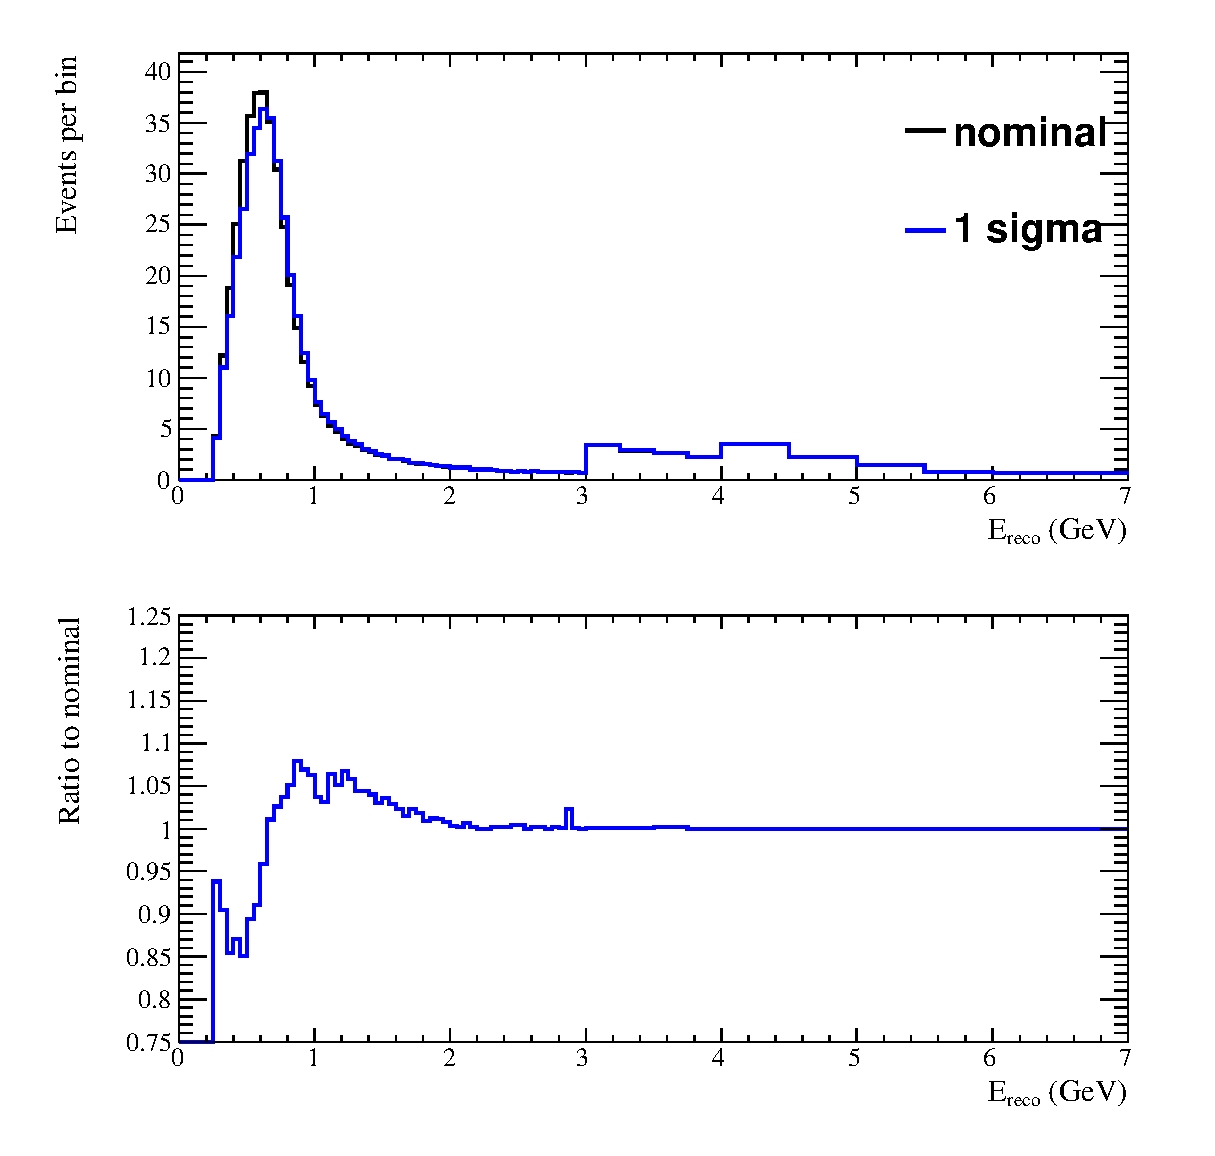
\includegraphics{../images/spectrum_tweaked/1sigma_unoscillated/ereco_twk_f_specfunc}}
\caption
{ Effect of $f_{SF; t, r}$ for no oscillations (all mixing angles set to 0). }
\label{fig:noosc_ereco_twk_f_specfunc}
\end{center}
\end{figure}
\clearpage

\begin{figure}
\begin{center}
\resizebox{14cm}{!}{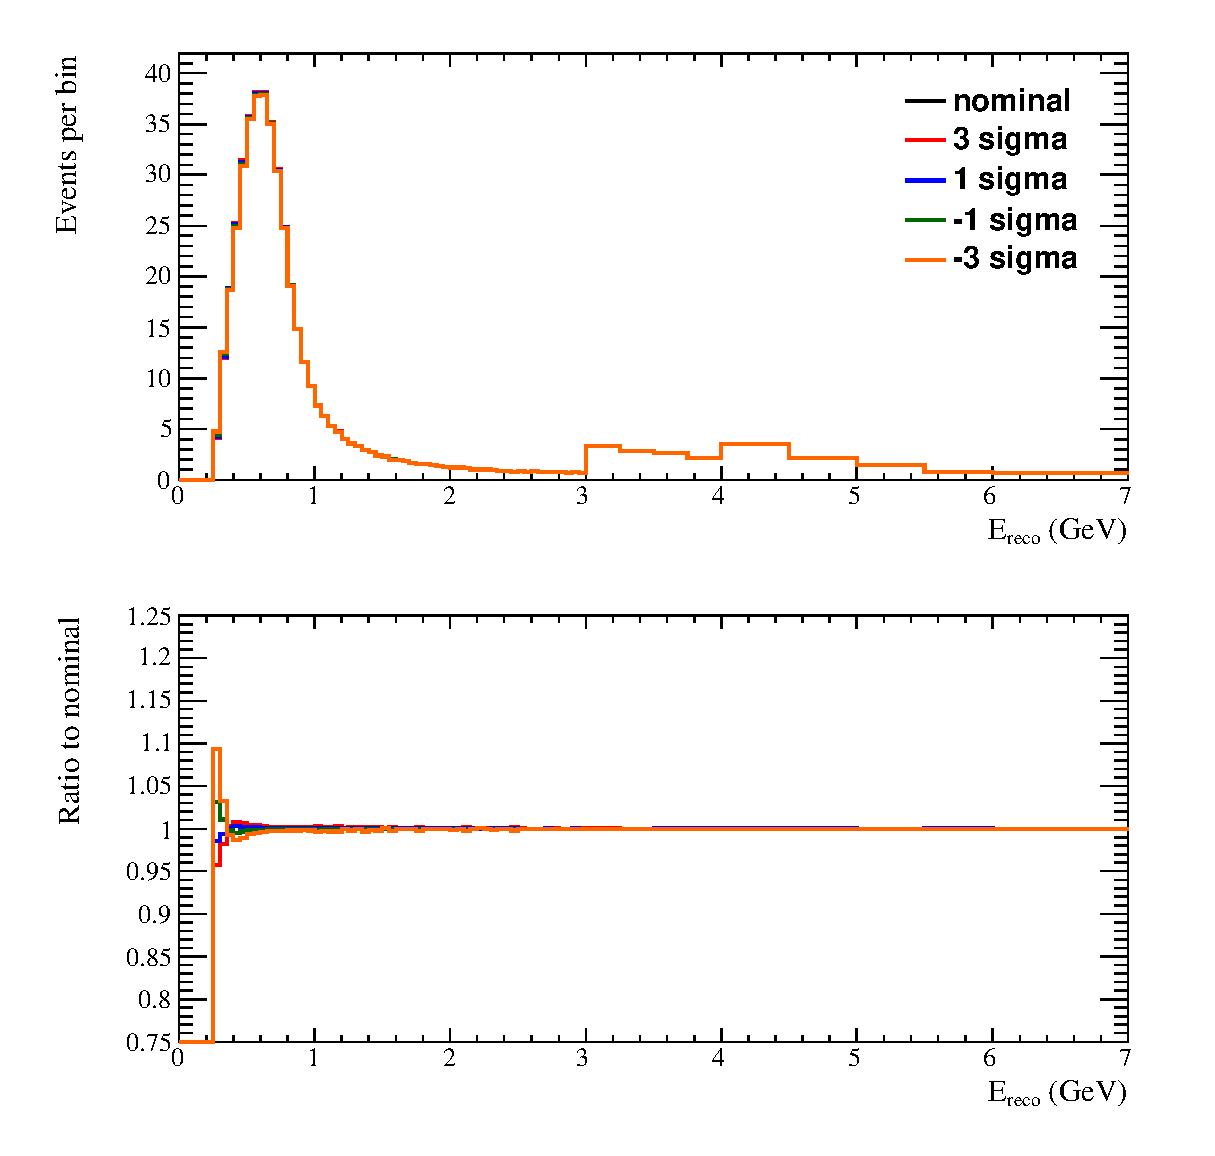
\includegraphics{../images/spectrum_tweaked/1sigma_unoscillated/ereco_twk_f_wshape}}
\caption
{ Effect of $f_{Wshape; t, r}$ for no oscillations (all mixing angles set to 0). }
\label{fig:noosc_ereco_twk_f_wshape}
\end{center}
\end{figure}
\clearpage

\begin{figure}
\begin{center}
\resizebox{14cm}{!}{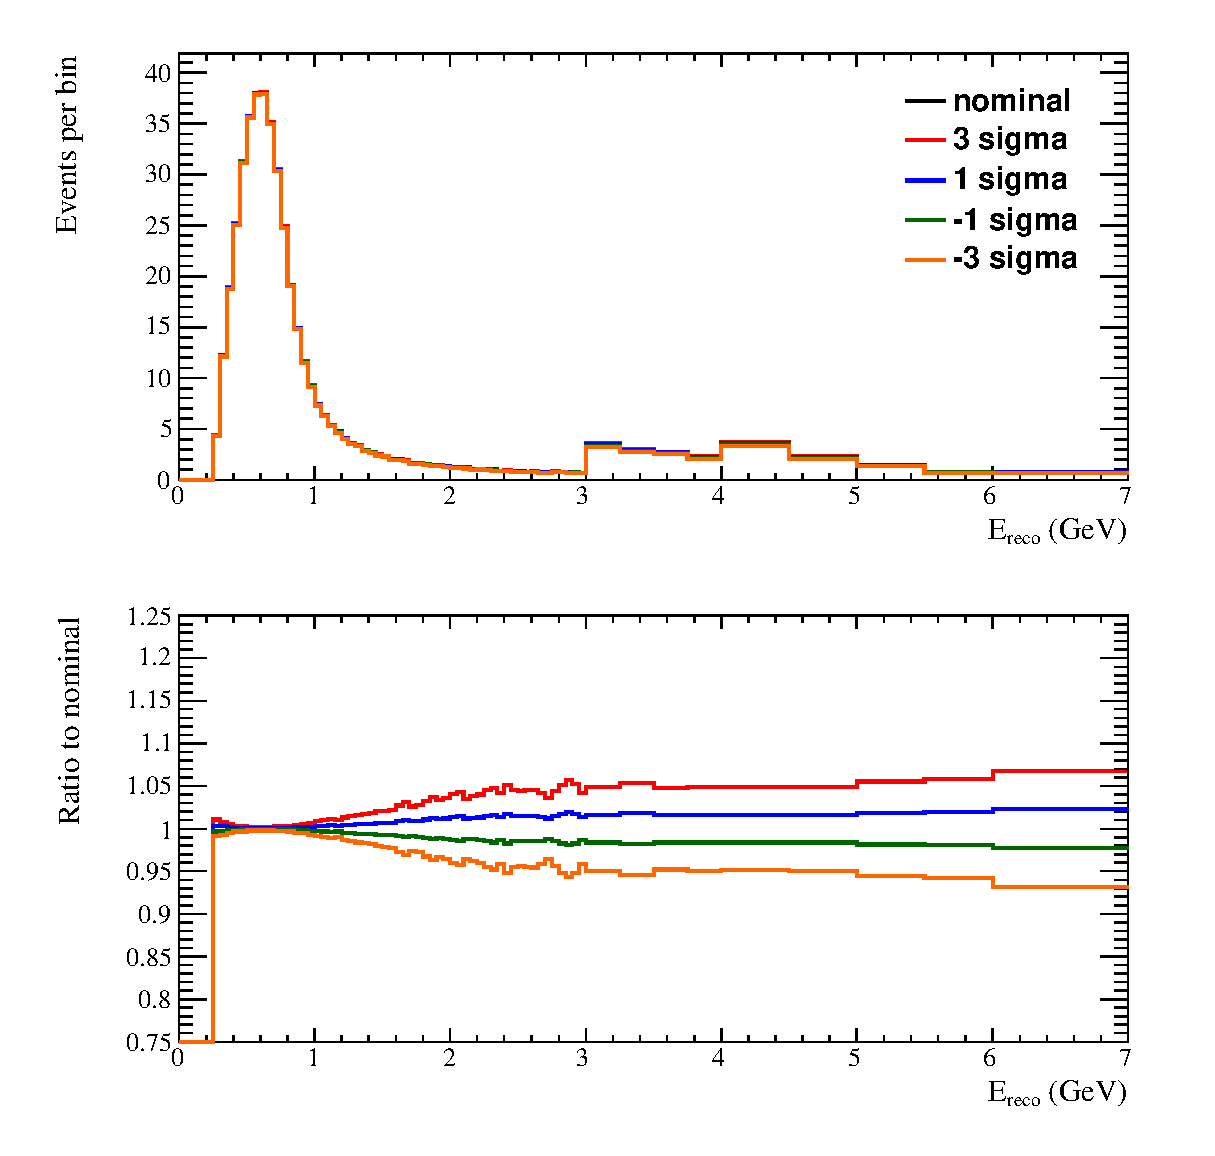
\includegraphics{../images/spectrum_tweaked/1sigma_unoscillated/ereco_twk_f_shapeCCoth}}
\caption
{ Effect of $f_{CCothShape; t, r}$ for no oscillations (all mixing angles set to 0). }
\label{fig:noosc_ereco_twk_f_shapeCCoth}
\end{center}
\end{figure}
\clearpage

\begin{figure}
\begin{center}
\resizebox{14cm}{!}{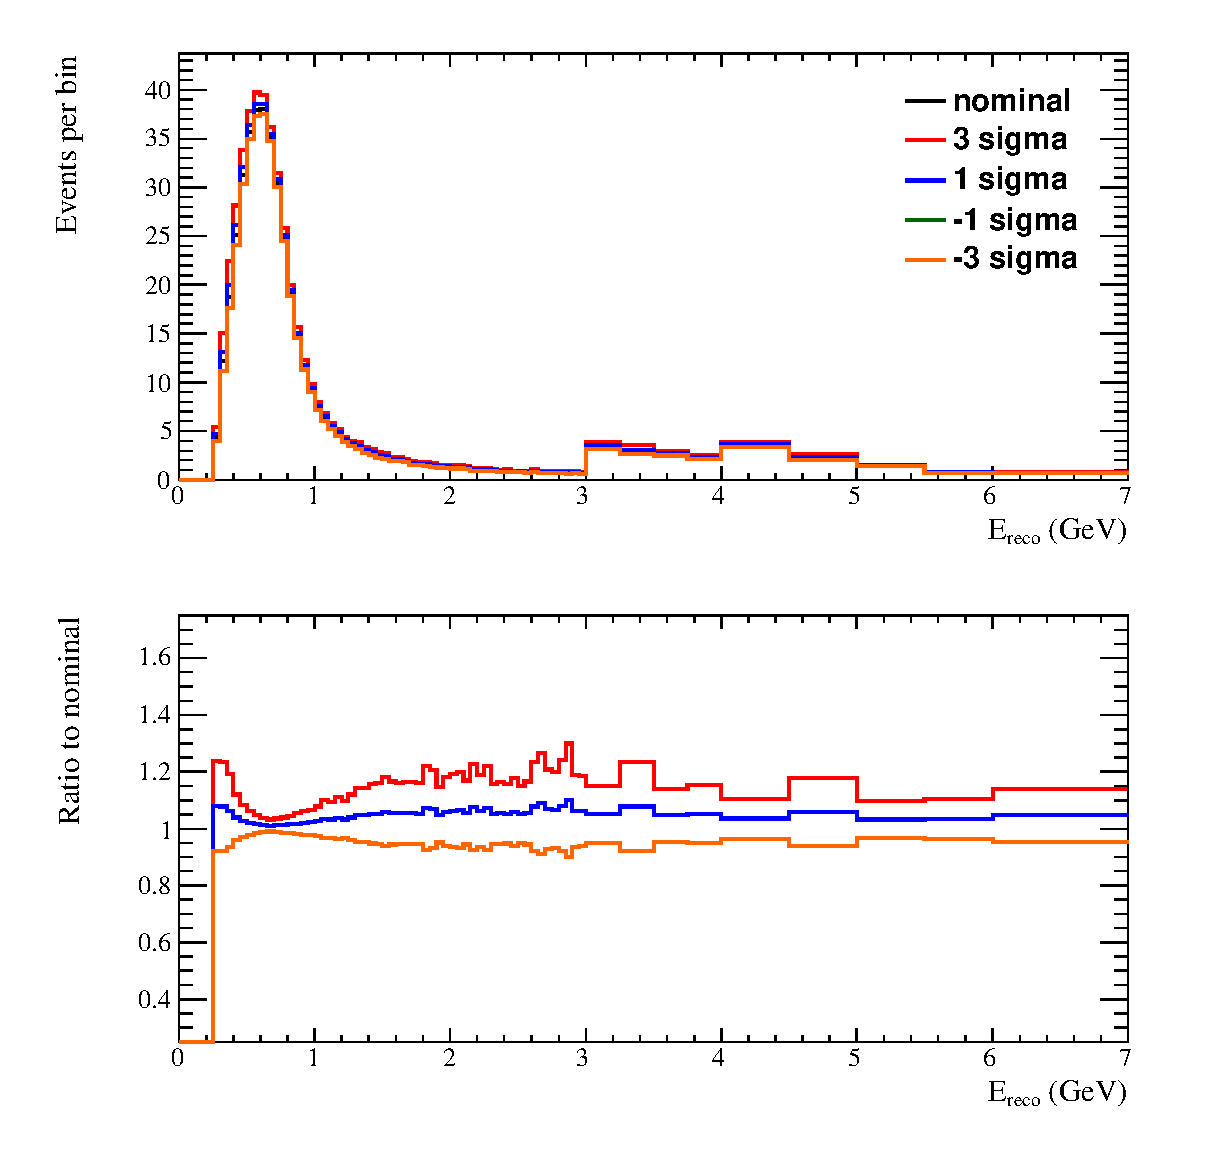
\includegraphics{../images/spectrum_tweaked/1sigma_unoscillated/ereco_twk_f_pilessdelta}}
\caption
{ Effect of $f_{\pi-less\Delta; t, r}$ for no oscillations (all mixing angles set to 0). }
\label{fig:noosc_ereco_twk_f_pilessdelta}
\end{center}
\end{figure}
\clearpage

\begin{figure}
\begin{center}
\resizebox{14cm}{!}{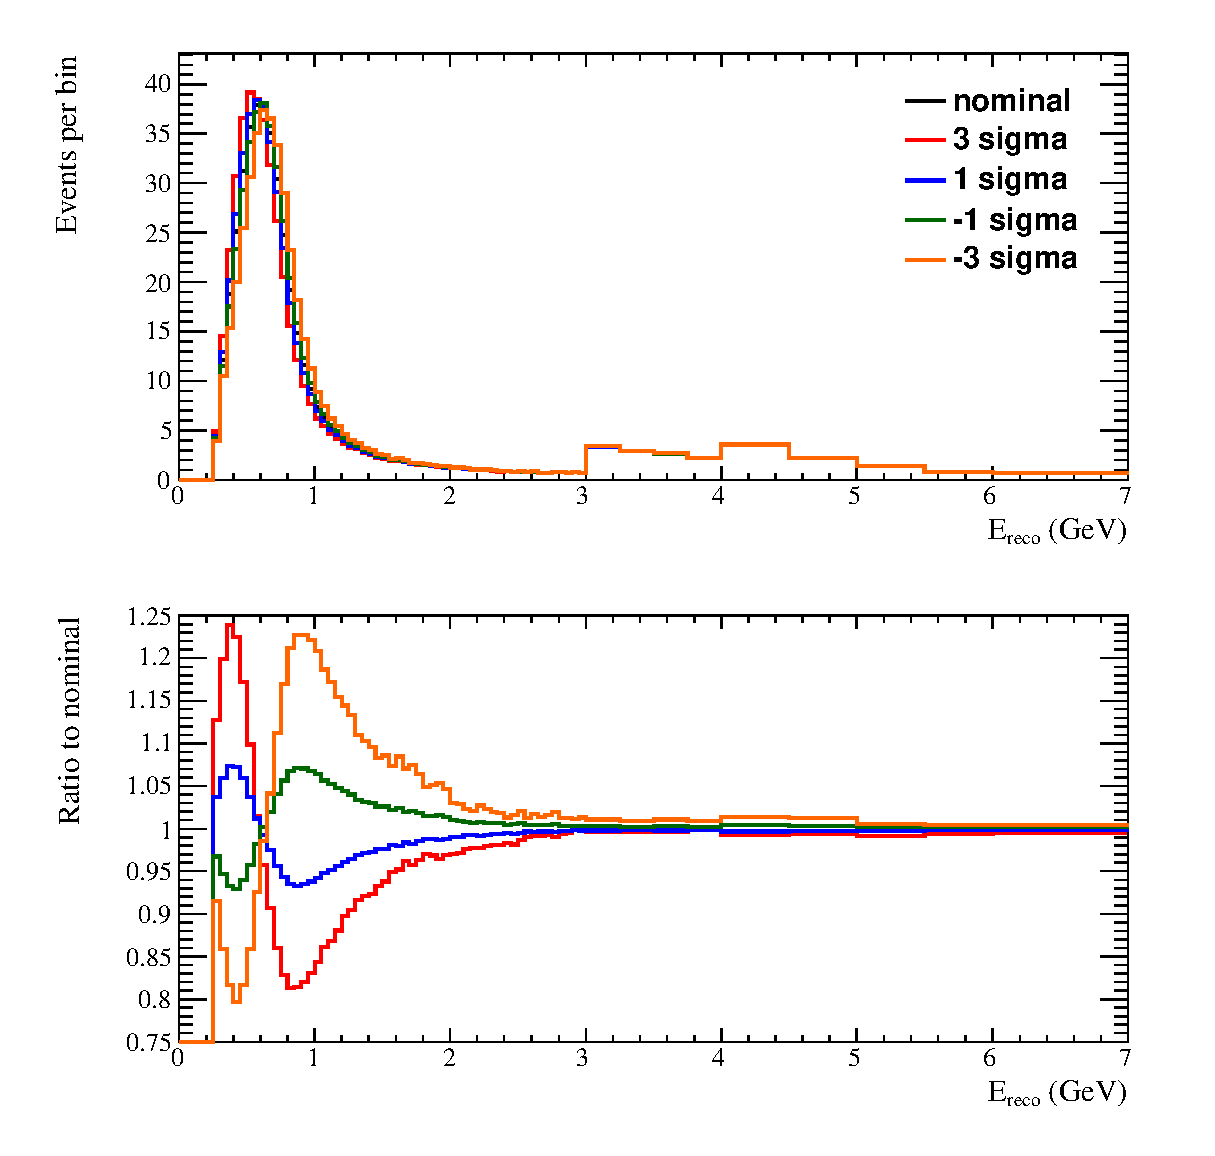
\includegraphics{../images/spectrum_tweaked/1sigma_unoscillated/ereco_twk_f_bindE}}
\caption
{ Effect of $f_{bindE; t, r}$ for no oscillations (all mixing angles set to 0). }
\label{fig:noosc_ereco_twk_f_bindE}
\end{center}
\end{figure}
\clearpage

\begin{figure}
\begin{center}
\resizebox{14cm}{!}{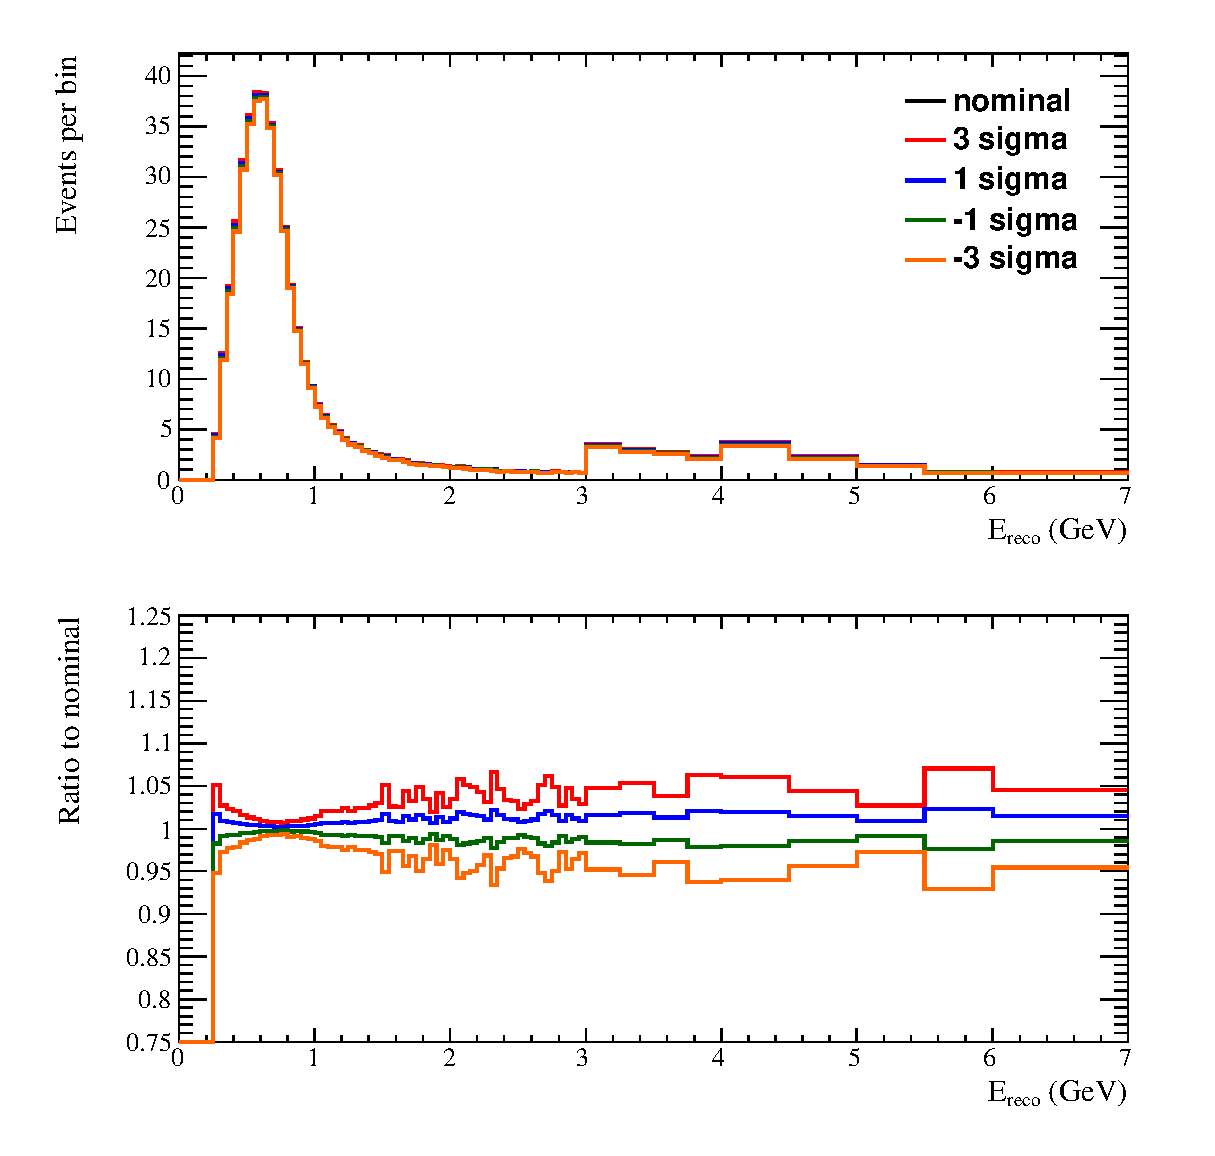
\includegraphics{../images/spectrum_tweaked/1sigma_unoscillated/ereco_twk_f_norm_cccoh}}
\caption
{ Effect of $f_{CCcoh; t}$ for no oscillations (all mixing angles set to 0). }
\label{fig:noosc_ereco_twk_f_norm_cccoh}
\end{center}
\end{figure}
\clearpage

\begin{figure}
\begin{center}
\resizebox{14cm}{!}{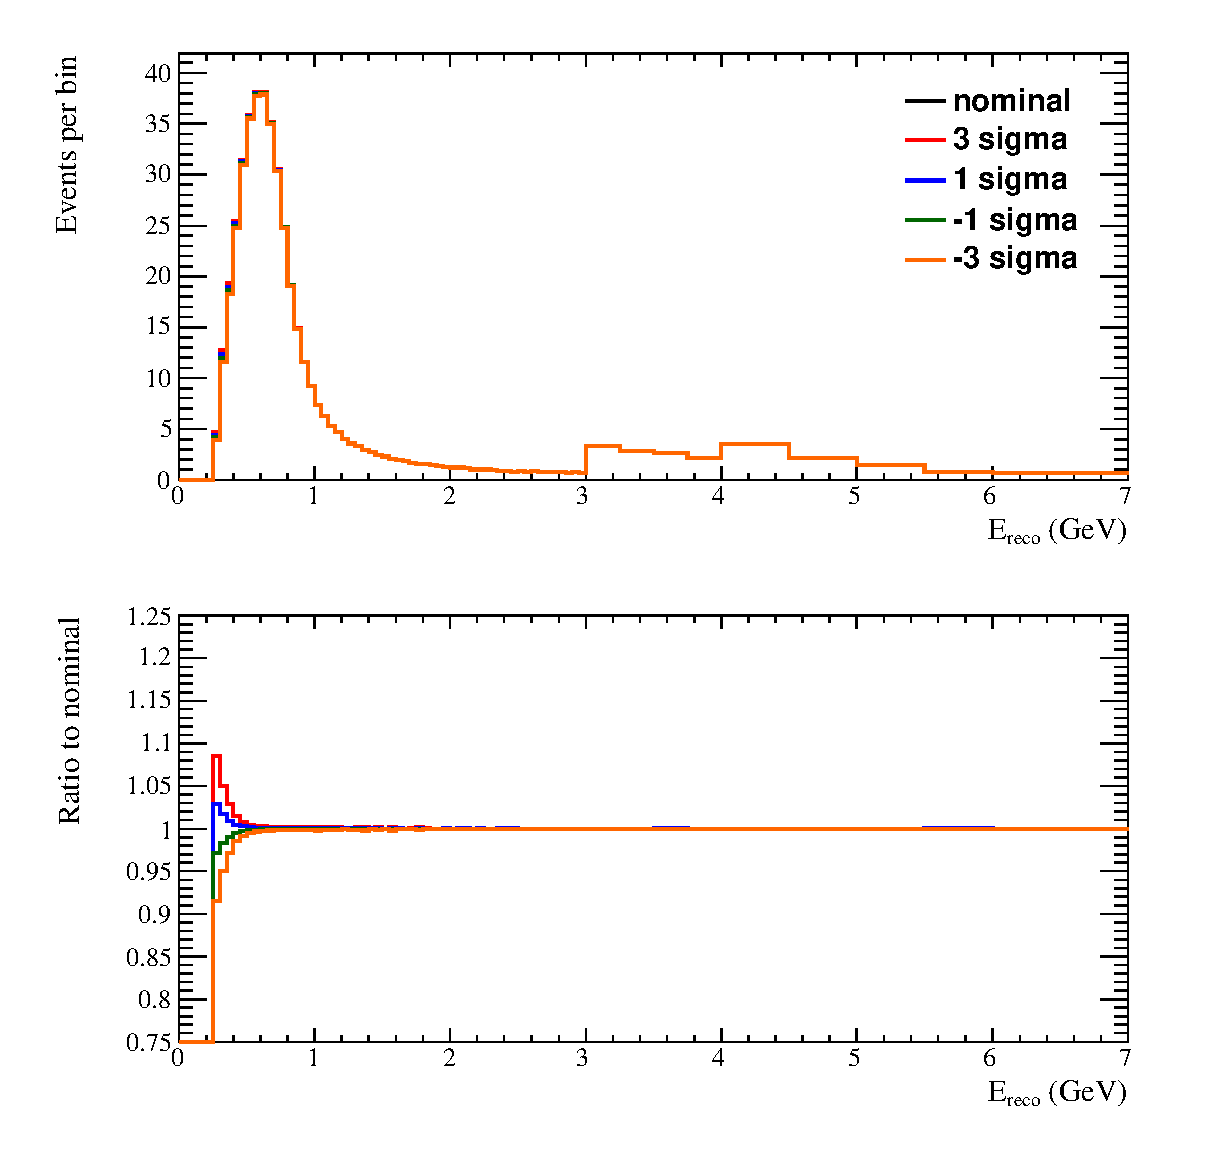
\includegraphics{../images/spectrum_tweaked/1sigma_unoscillated/ereco_twk_f_norm_nc1piC}}
\caption
{ Effect of $f_{NC1\pi^\pm; t}$ for no oscillations (all mixing angles set to 0). }
\label{fig:noosc_ereco_twk_f_norm_nc1piC}
\end{center}
\end{figure}
\clearpage

\begin{figure}
\begin{center}
\resizebox{14cm}{!}{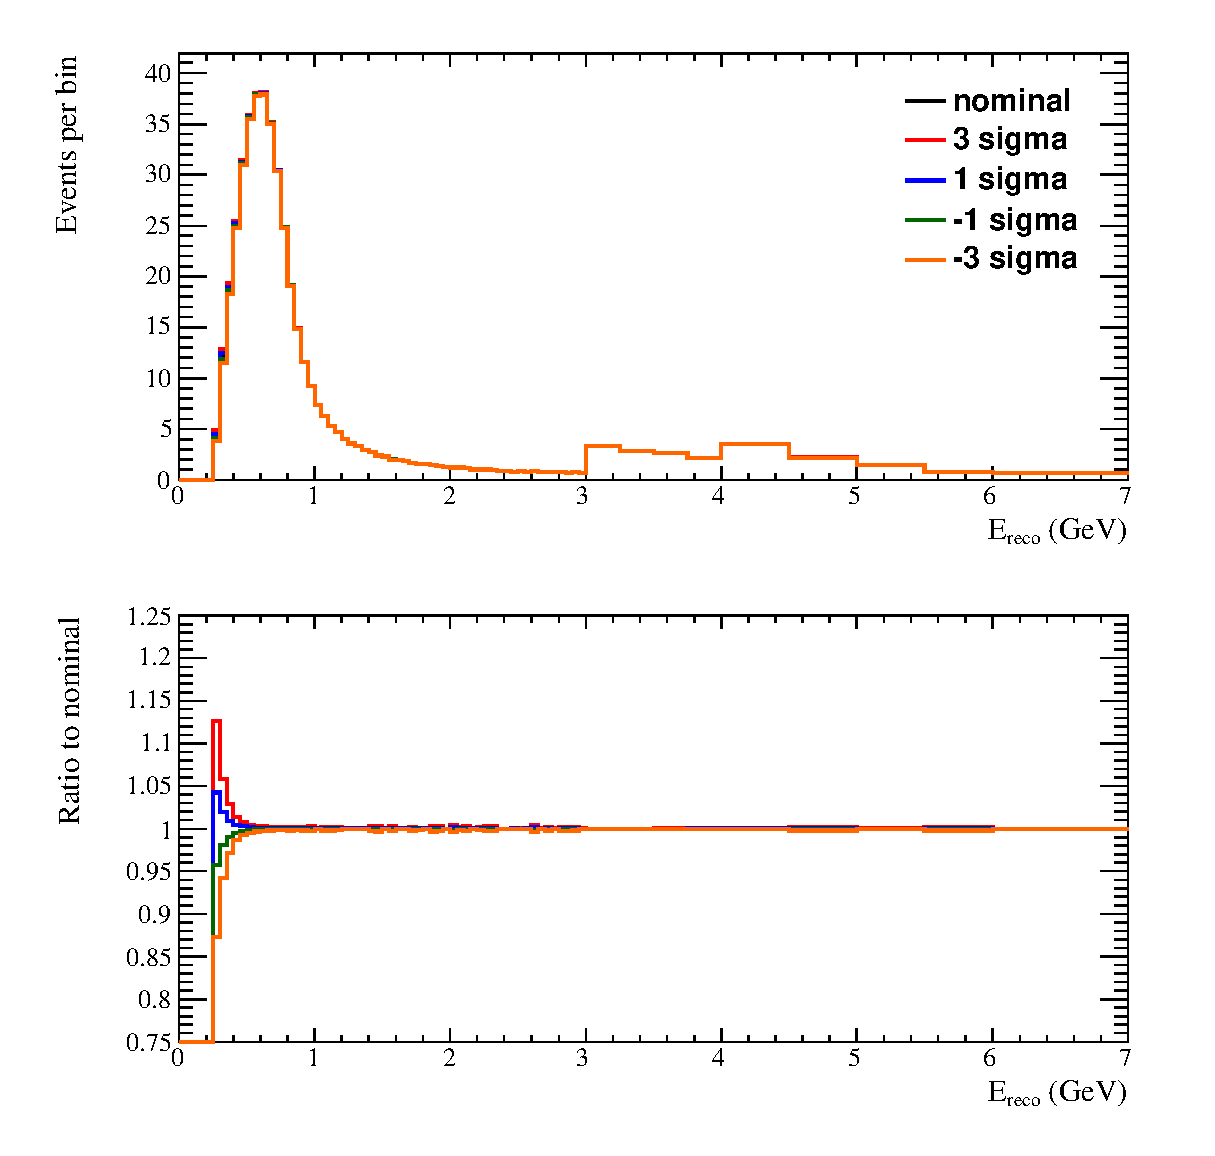
\includegraphics{../images/spectrum_tweaked/1sigma_unoscillated/ereco_twk_f_norm_ncoth}}
\caption
{ Effect of $f_{NCoth; t}$ for no oscillations (all mixing angles set to 0). }
\label{fig:noosc_ereco_twk_f_norm_ncoth}
\end{center}
\end{figure}
\clearpage

\begin{figure}
\begin{center}
\resizebox{14cm}{!}{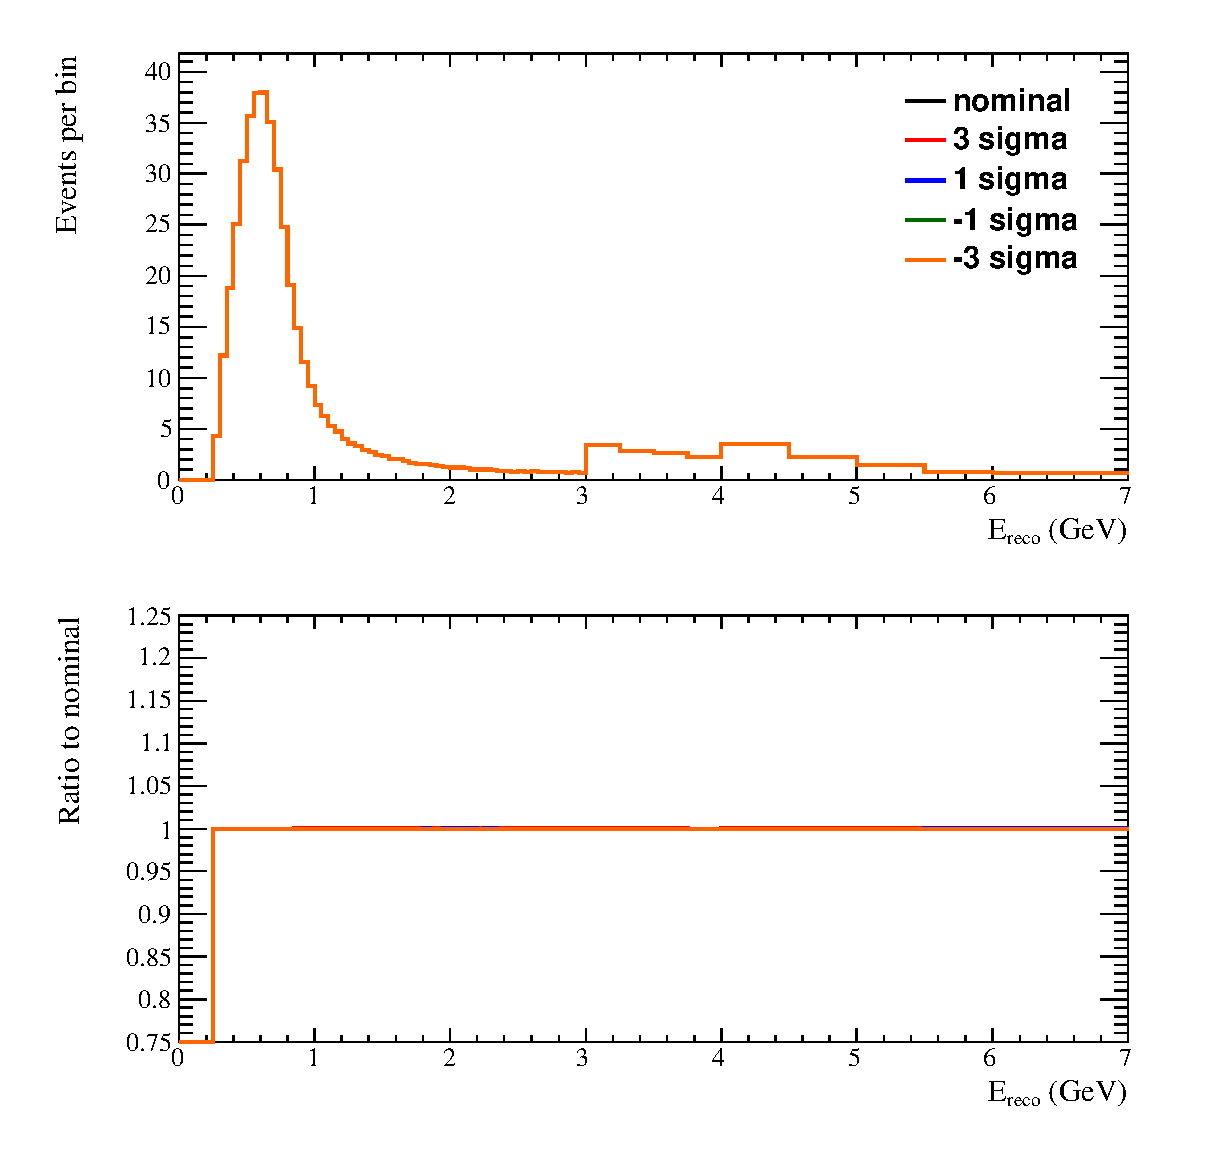
\includegraphics{../images/spectrum_tweaked/1sigma_unoscillated/ereco_twk_f_norm_nuetonumu}}
\caption
{ Effect of $f_{CC\nu_e; t}$ for no oscillations (all mixing angles set to 0). }
\label{fig:noosc_ereco_twk_f_norm_nuetonumu}
\end{center}
\end{figure}
\clearpage

\begin{figure}
\begin{center}
\resizebox{14cm}{!}{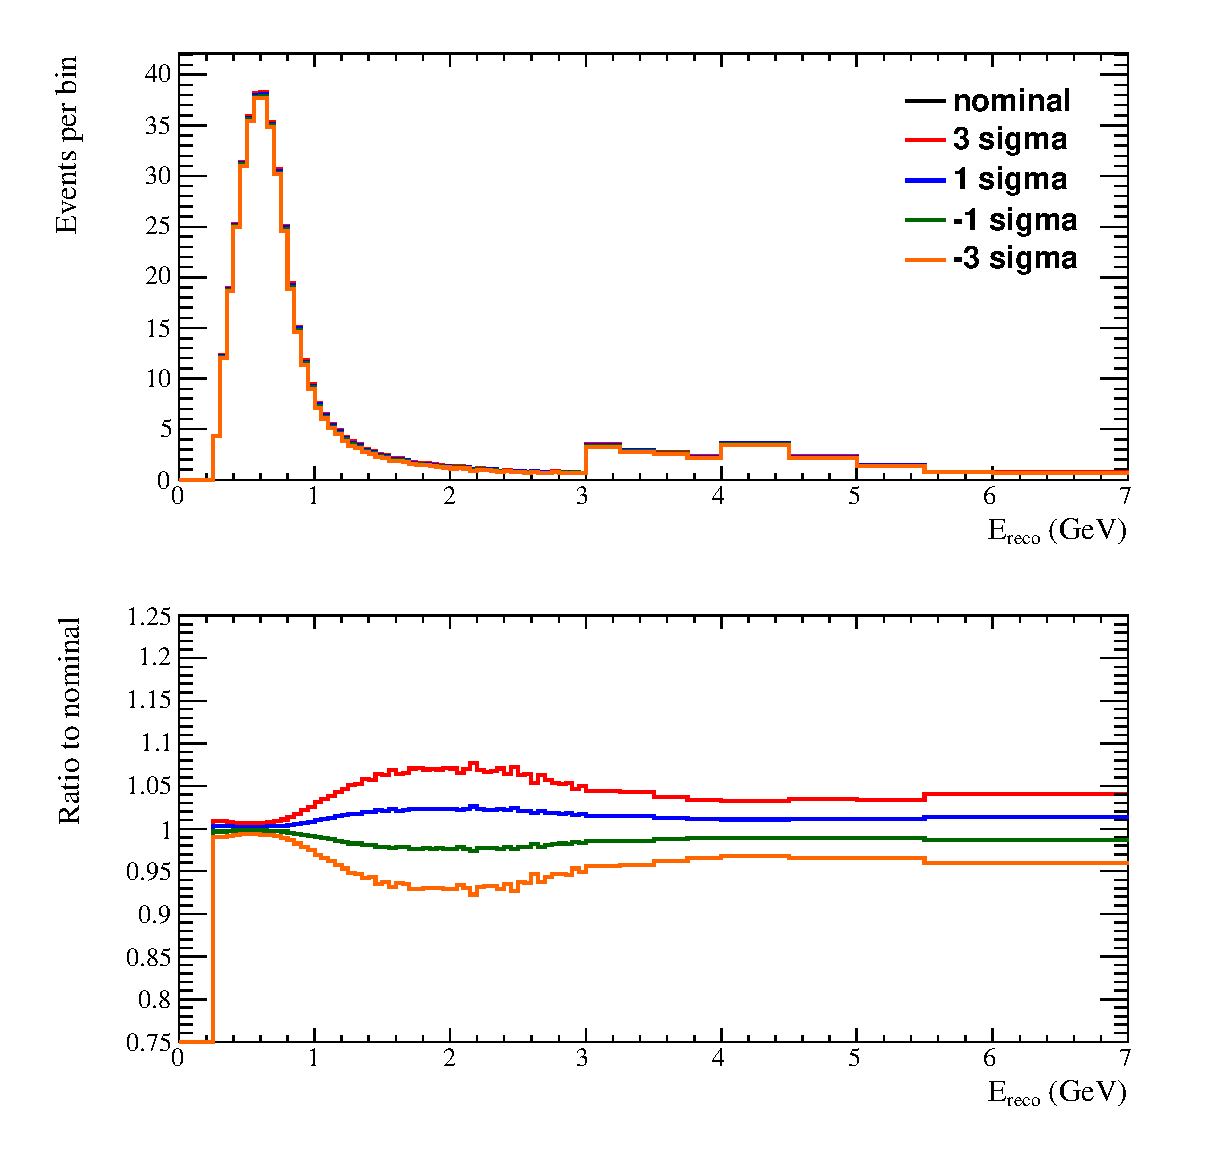
\includegraphics{../images/spectrum_tweaked/1sigma_unoscillated/ereco_twk_f_norm_antinutonu}}
\caption
{ Effect of $f_{CC\bar{\nu}; t}$ for no oscillations (all mixing angles set to 0). }
\label{fig:noosc_ereco_twk_f_norm_antinutonu}
\end{center}
\end{figure}
\clearpage

\begin{figure}
\begin{center}
\resizebox{14cm}{!}{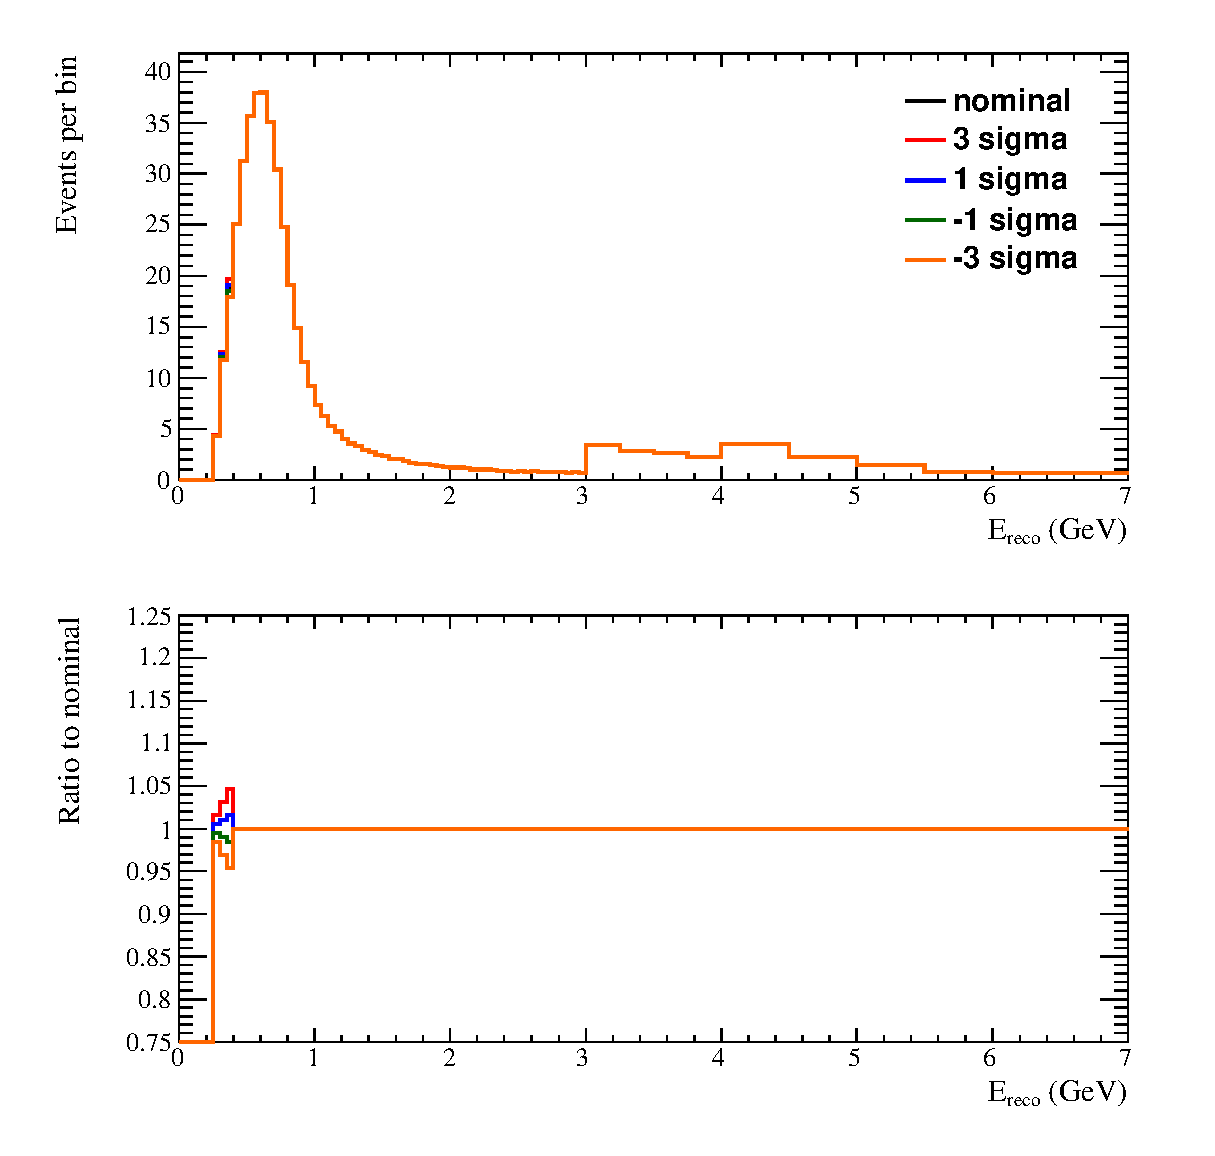
\includegraphics{../images/spectrum_tweaked/1sigma_unoscillated/ereco_twk_f_skdetfsi000}}
\caption
{ Effect of $f_{0; r}^{SK+FSI}$ for no oscillations (all mixing angles set to 0). }
\label{fig:noosc_ereco_twk_f_skdetfsi000}
\end{center}
\end{figure}
\clearpage

\begin{figure}
\begin{center}
\resizebox{14cm}{!}{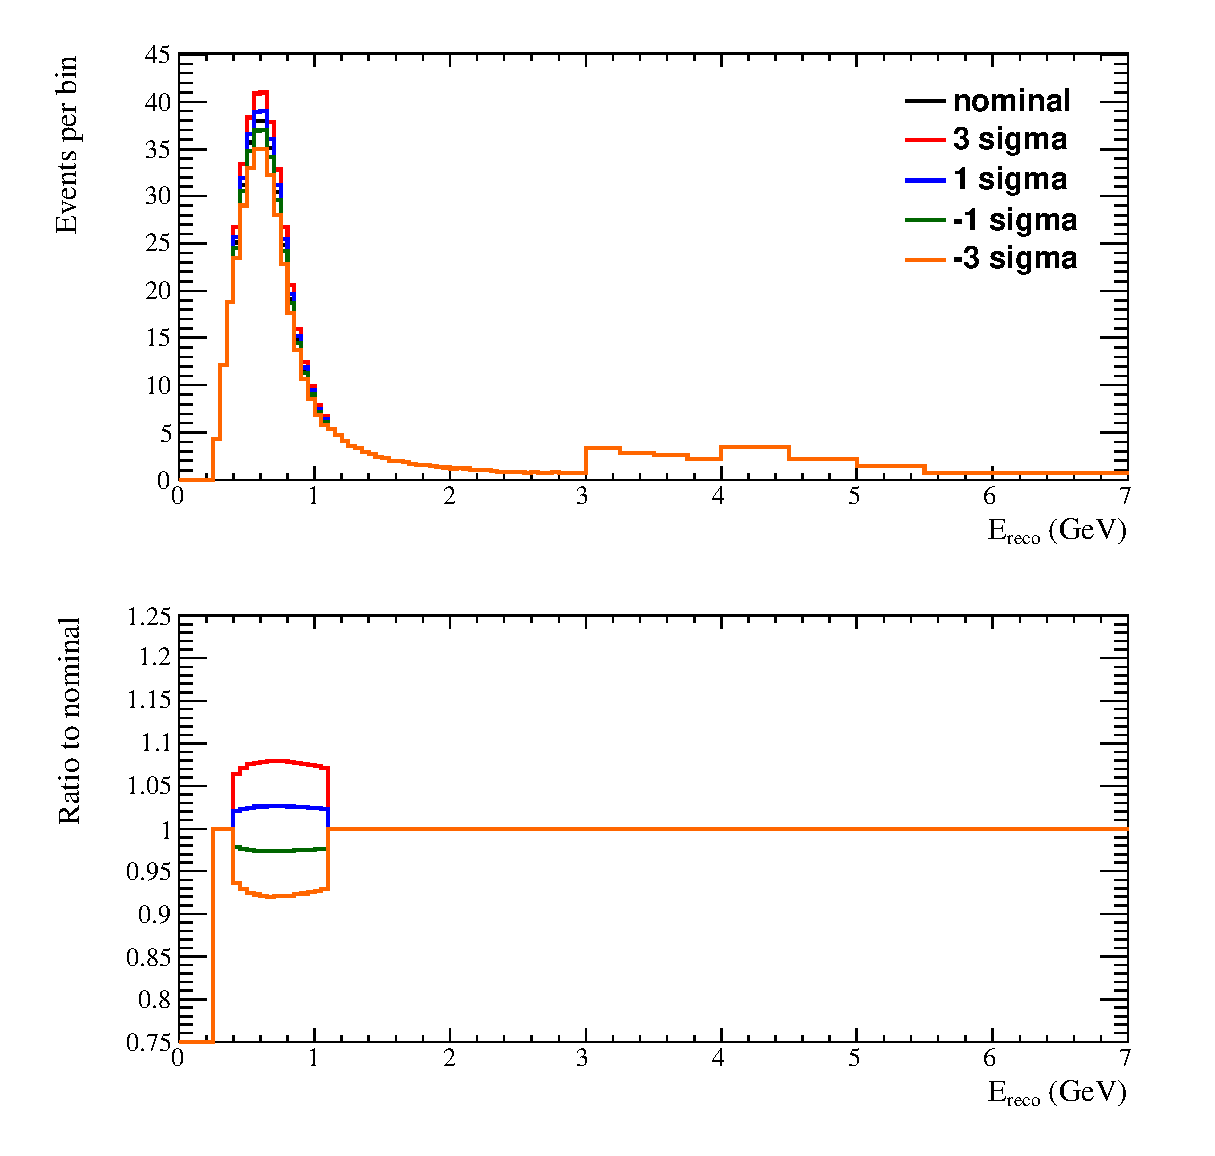
\includegraphics{../images/spectrum_tweaked/1sigma_unoscillated/ereco_twk_f_skdetfsi001}}
\caption
{ Effect of $f_{1; r}^{SK+FSI}$ for no oscillations (all mixing angles set to 0). }
\label{fig:noosc_ereco_twk_f_skdetfsi001}
\end{center}
\end{figure}
\clearpage

\begin{figure}
\begin{center}
\resizebox{14cm}{!}{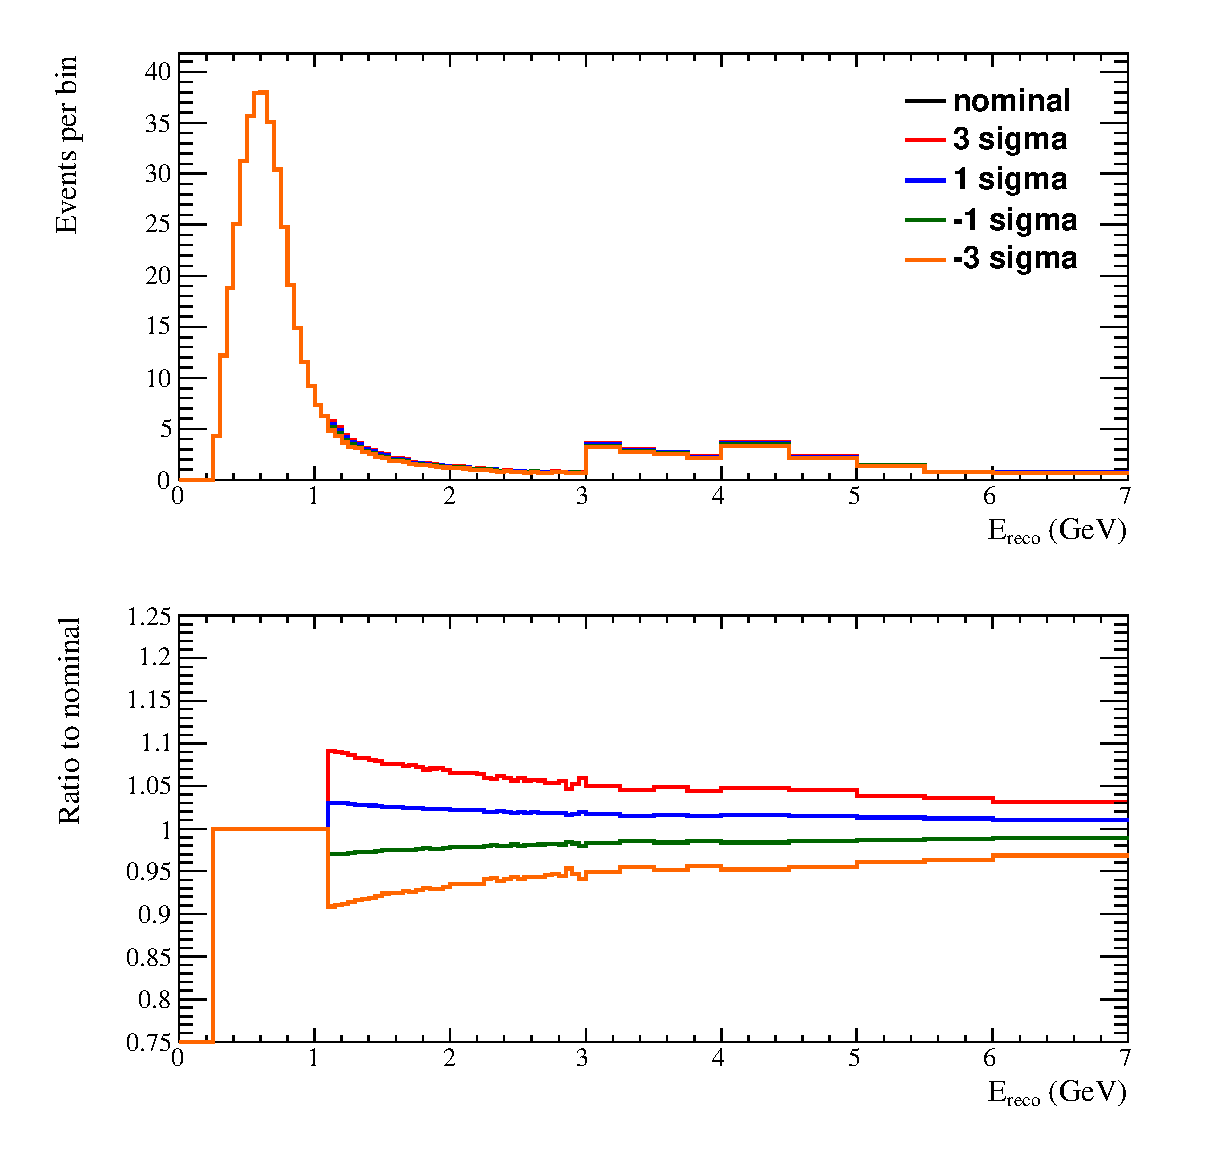
\includegraphics{../images/spectrum_tweaked/1sigma_unoscillated/ereco_twk_f_skdetfsi002}}
\caption
{ Effect of $f_{2; r}^{SK+FSI}$ for no oscillations (all mixing angles set to 0). }
\label{fig:noosc_ereco_twk_f_skdetfsi002}
\end{center}
\end{figure}
\clearpage

\begin{figure}
\begin{center}
\resizebox{14cm}{!}{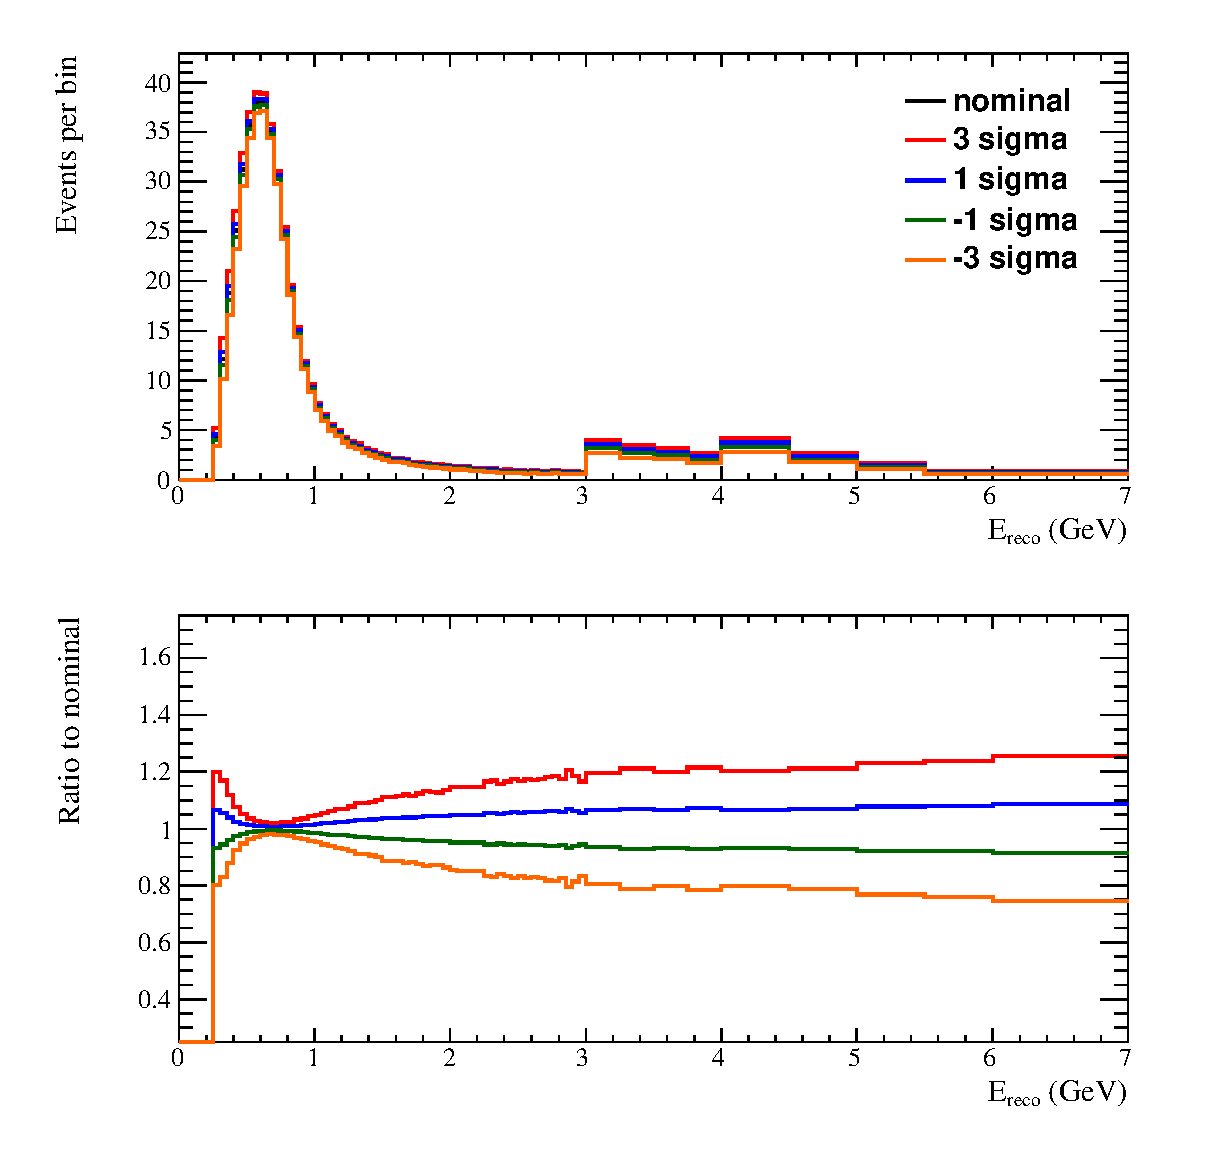
\includegraphics{../images/spectrum_tweaked/1sigma_unoscillated/ereco_twk_f_skdetfsi003}}
\caption
{ Effect of $f_{3; r}^{SK+FSI}$ for no oscillations (all mixing angles set to 0). }
\label{fig:noosc_ereco_twk_f_skdetfsi003}
\end{center}
\end{figure}
\clearpage

\begin{figure}
\begin{center}
\resizebox{14cm}{!}{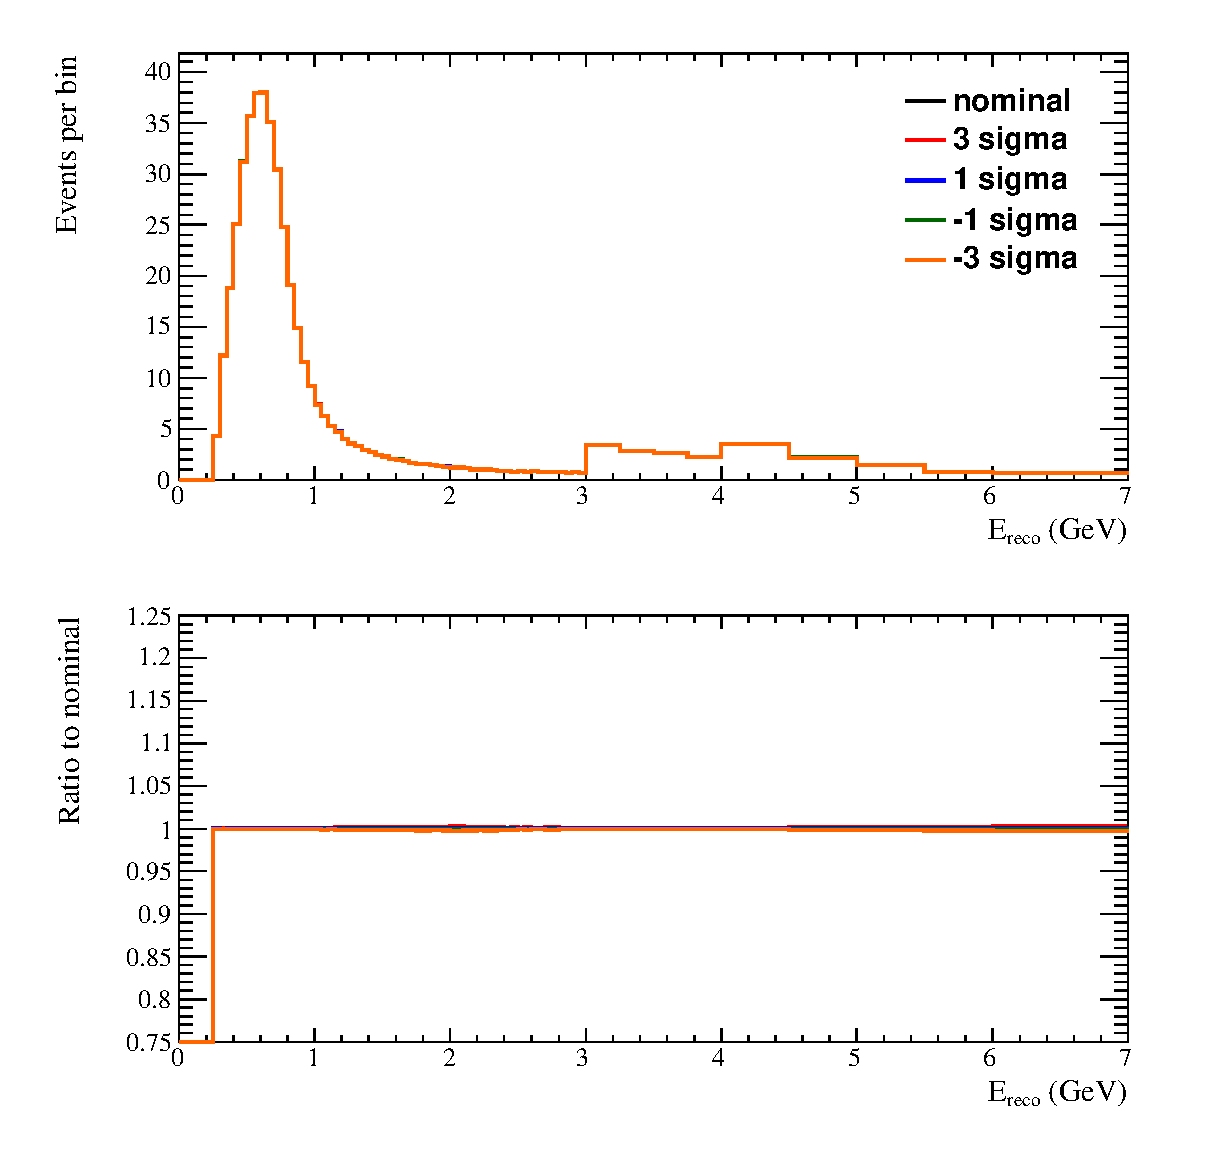
\includegraphics{../images/spectrum_tweaked/1sigma_unoscillated/ereco_twk_f_skdetfsi004}}
\caption
{ Effect of $f_{4; r}^{SK+FSI}$ for no oscillations (all mixing angles set to 0). }
\label{fig:noosc_ereco_twk_f_skdetfsi004}
\end{center}
\end{figure}
\clearpage

\begin{figure}
\begin{center}
\resizebox{14cm}{!}{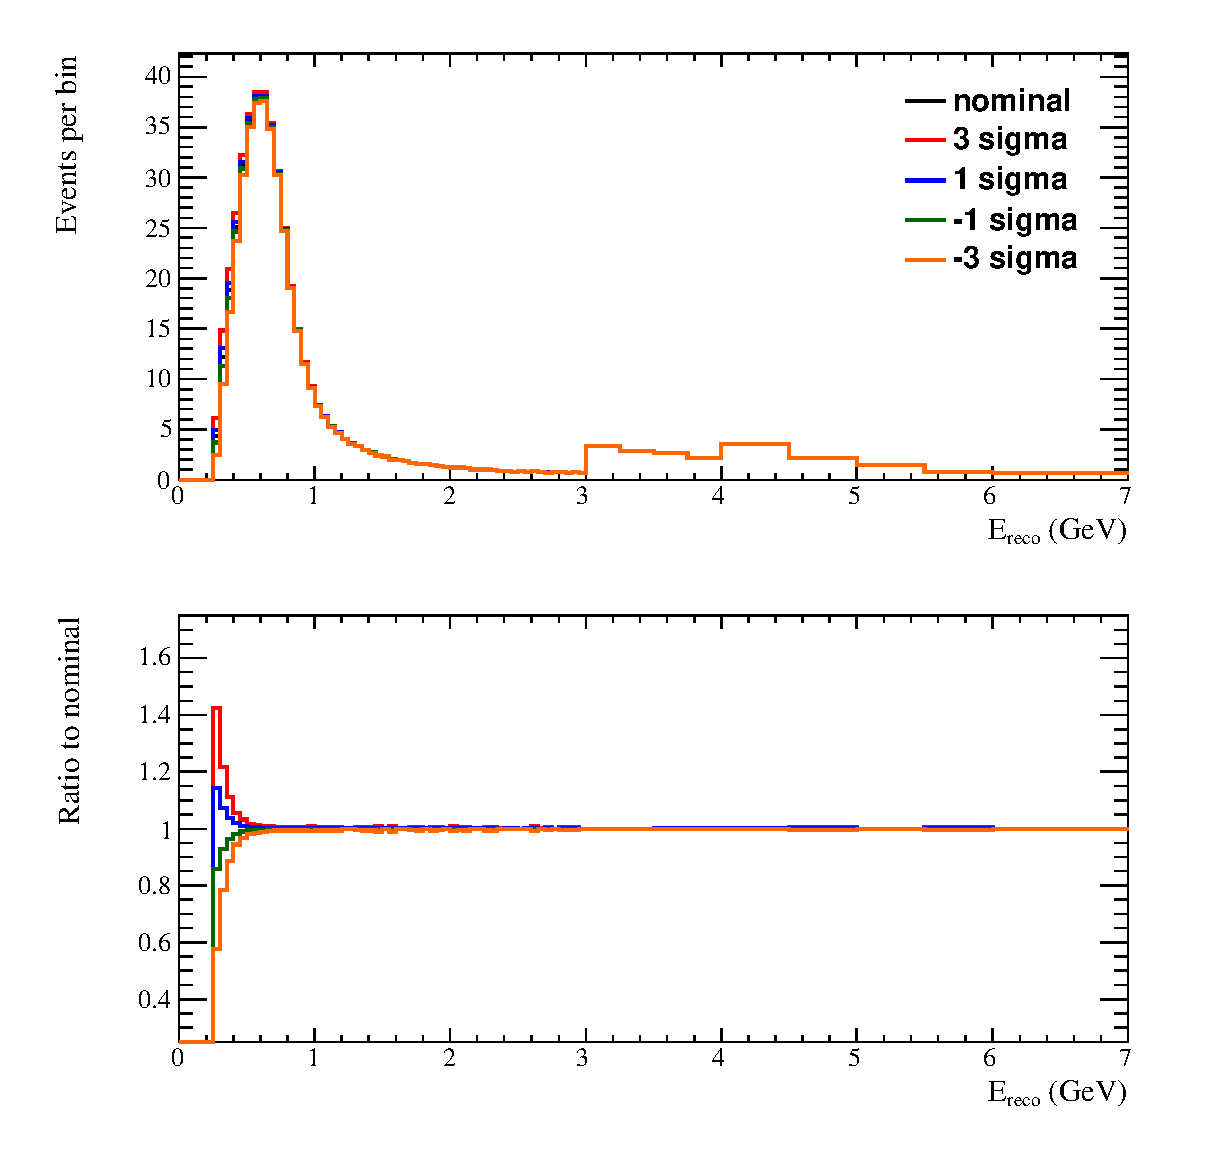
\includegraphics{../images/spectrum_tweaked/1sigma_unoscillated/ereco_twk_f_skdetfsi005}}
\caption
{ Effect of $f_{5; r}^{SK+FSI}$ for no oscillations (all mixing angles set to 0). }
\label{fig:noosc_ereco_twk_f_skdetfsi005}
\end{center}
\end{figure}
\clearpage



\begin{figure}
\begin{center}
\resizebox{14cm}{!}{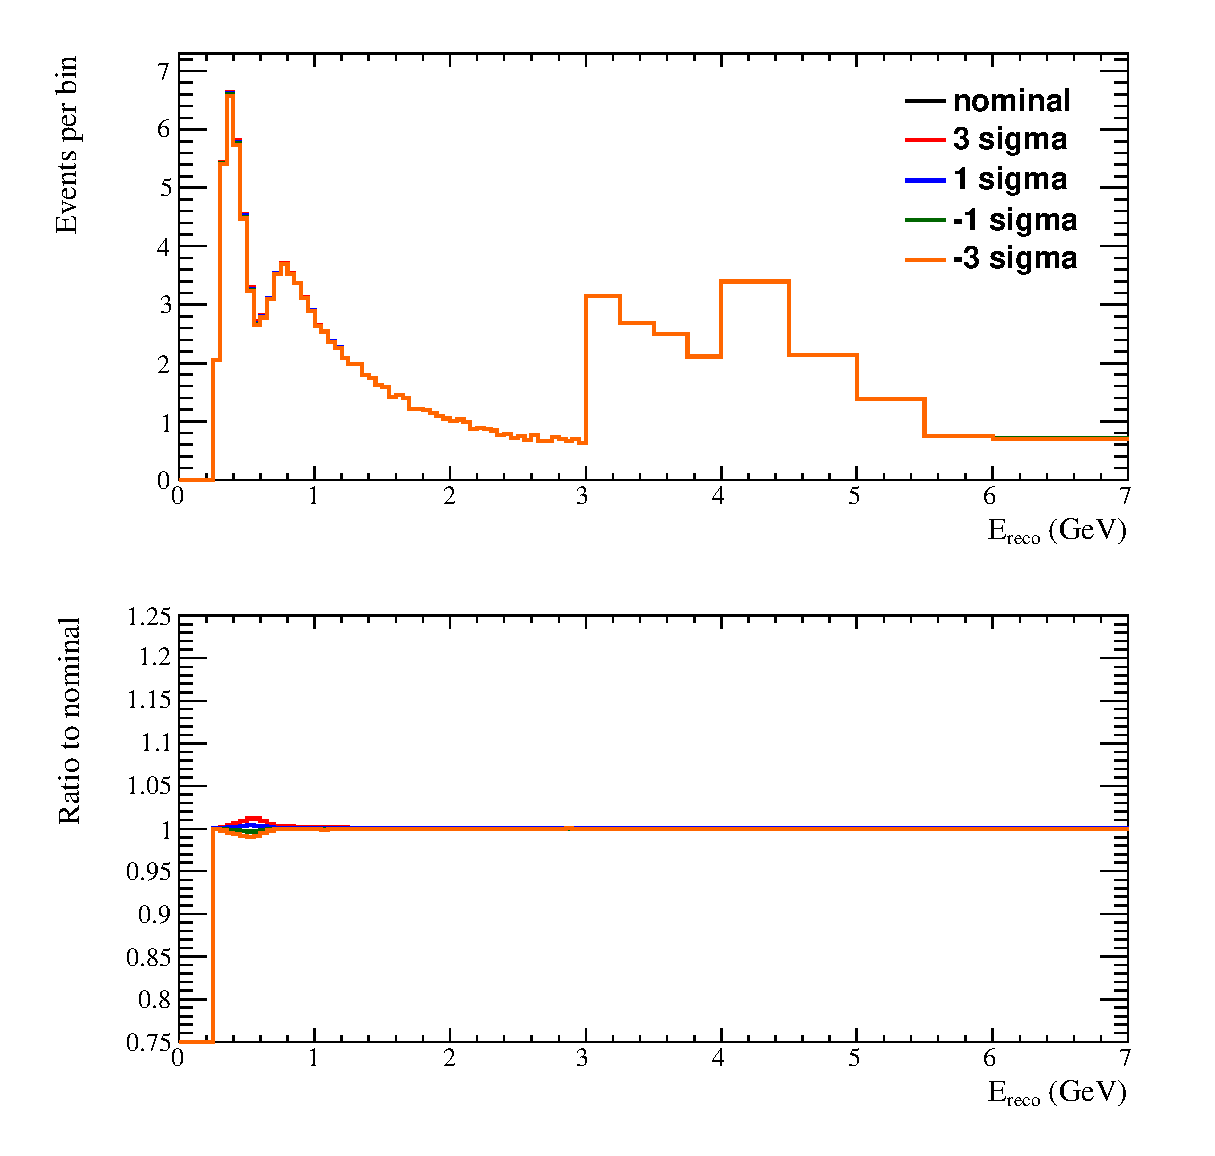
\includegraphics{../images/spectrum_tweaked/1sigma_oscillated/ereco_twk_sinsqtheta13}}
\caption
{ Effect of $\sin^2(\theta_{13})$ for 3 flavour oscillations, using oscillation parameters:  $\sin^2\theta_{12} = $0.306; $\sin^2\theta_{13} = $0.0251; $\sin^2\theta_{23} = $0.5; $\delta_{CP} = $        0; $\Delta m^2_{21} = $    7.5e-05 eV$^2$/c$^4$; $|\Delta m^2_{32}| = $    0.0024 eV$^2$/c$^4$. }
\label{fig:osc_ereco_twk_sinsqtheta13}
\end{center}
\end{figure}
\clearpage

\begin{figure}
\begin{center}
\resizebox{14cm}{!}{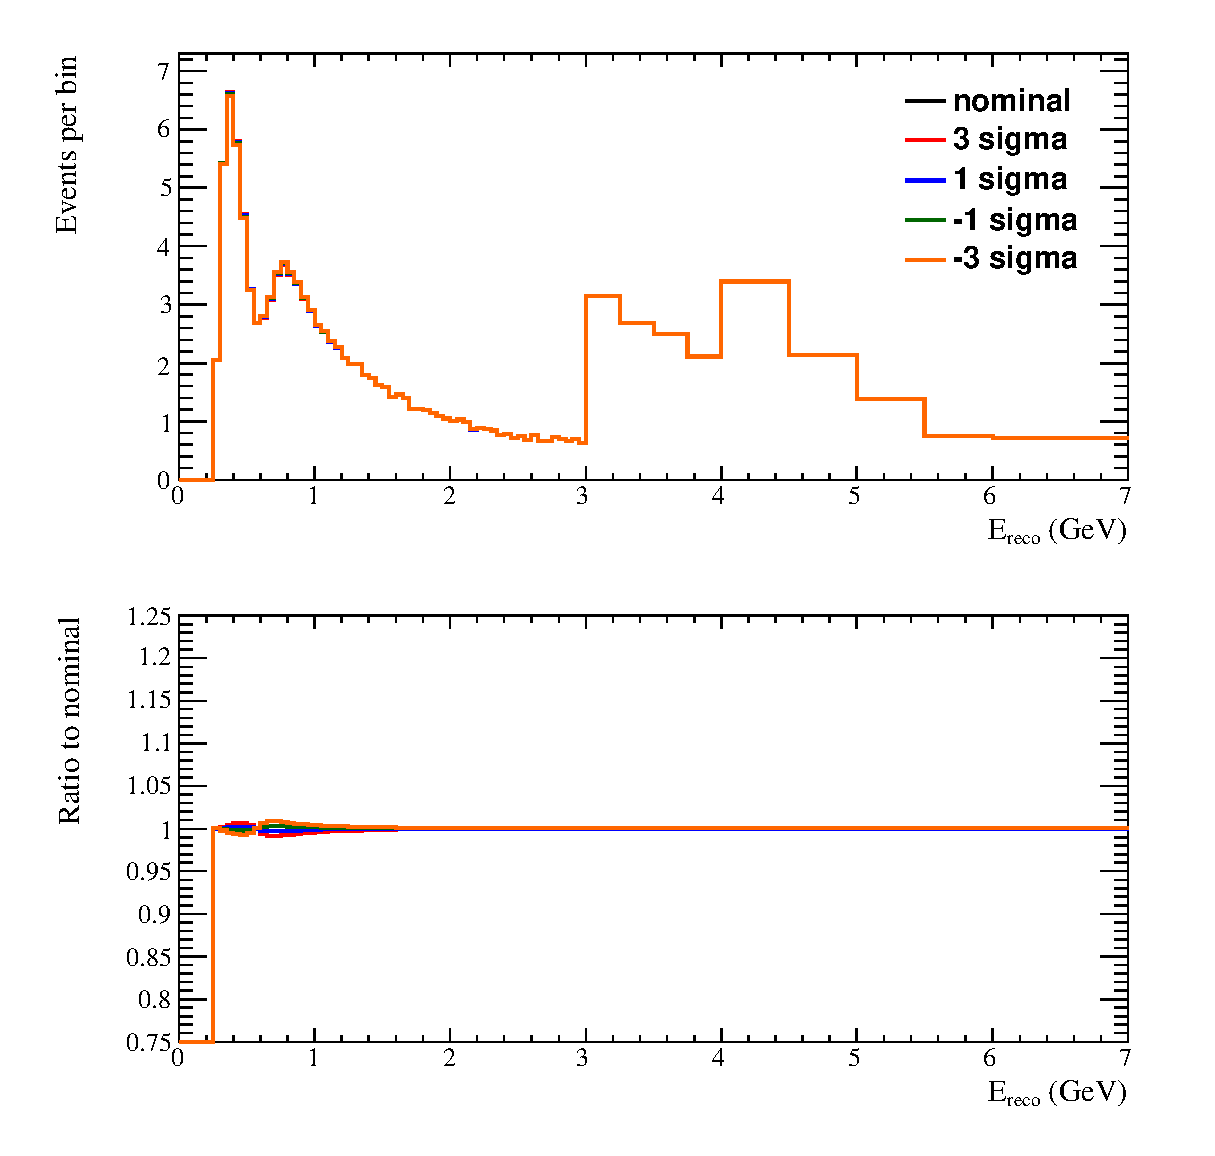
\includegraphics{../images/spectrum_tweaked/1sigma_oscillated/ereco_twk_sinsqtheta12}}
\caption
{ Effect of $\sin^2(\theta_{12})$ for 3 flavour oscillations, using oscillation parameters:  $\sin^2\theta_{12} = $0.306; $\sin^2\theta_{13} = $0.0251; $\sin^2\theta_{23} = $0.5; $\delta_{CP} = $        0; $\Delta m^2_{21} = $    7.5e-05 eV$^2$/c$^4$; $|\Delta m^2_{32}| = $    0.0024 eV$^2$/c$^4$. }
\label{fig:osc_ereco_twk_sinsqtheta12}
\end{center}
\end{figure}
\clearpage

\begin{figure}
\begin{center}
\resizebox{14cm}{!}{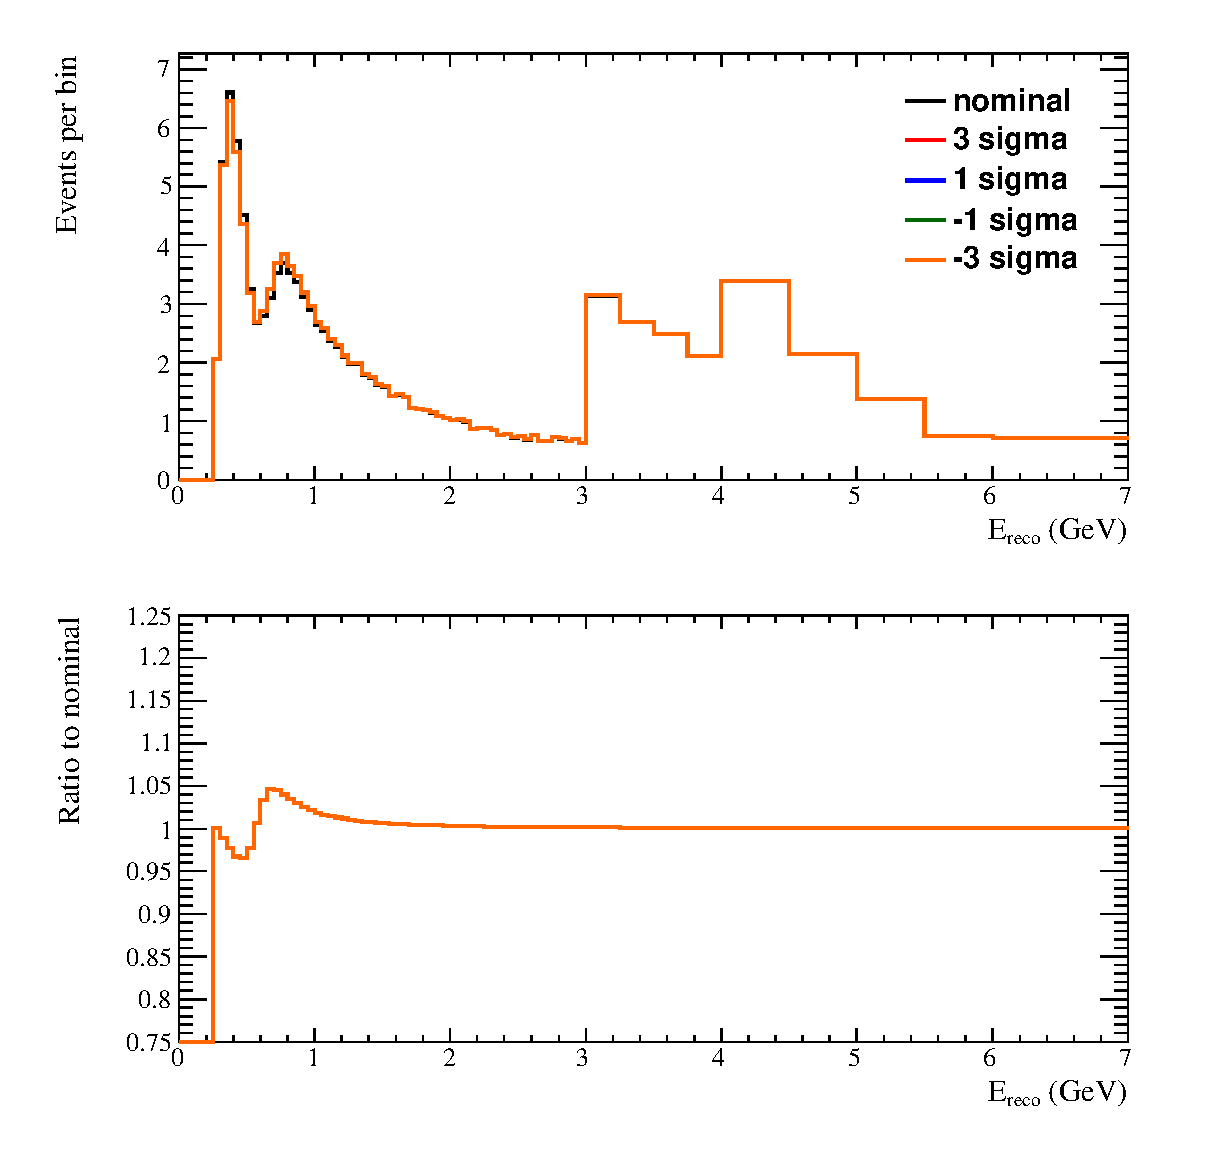
\includegraphics{../images/spectrum_tweaked/1sigma_oscillated/ereco_twk_delta_cp}}
\caption
{ Effect of $\delta_{CP}$ for 3 flavour oscillations, using oscillation parameters:  $\sin^2\theta_{12} = $0.306; $\sin^2\theta_{13} = $0.0251; $\sin^2\theta_{23} = $0.5; $\delta_{CP} = $        0; $\Delta m^2_{21} = $    7.5e-05 eV$^2$/c$^4$; $|\Delta m^2_{32}| = $    0.0024 eV$^2$/c$^4$. }
\label{fig:osc_ereco_twk_delta_cp}
\end{center}
\end{figure}
\clearpage

\begin{figure}
\begin{center}
\resizebox{14cm}{!}{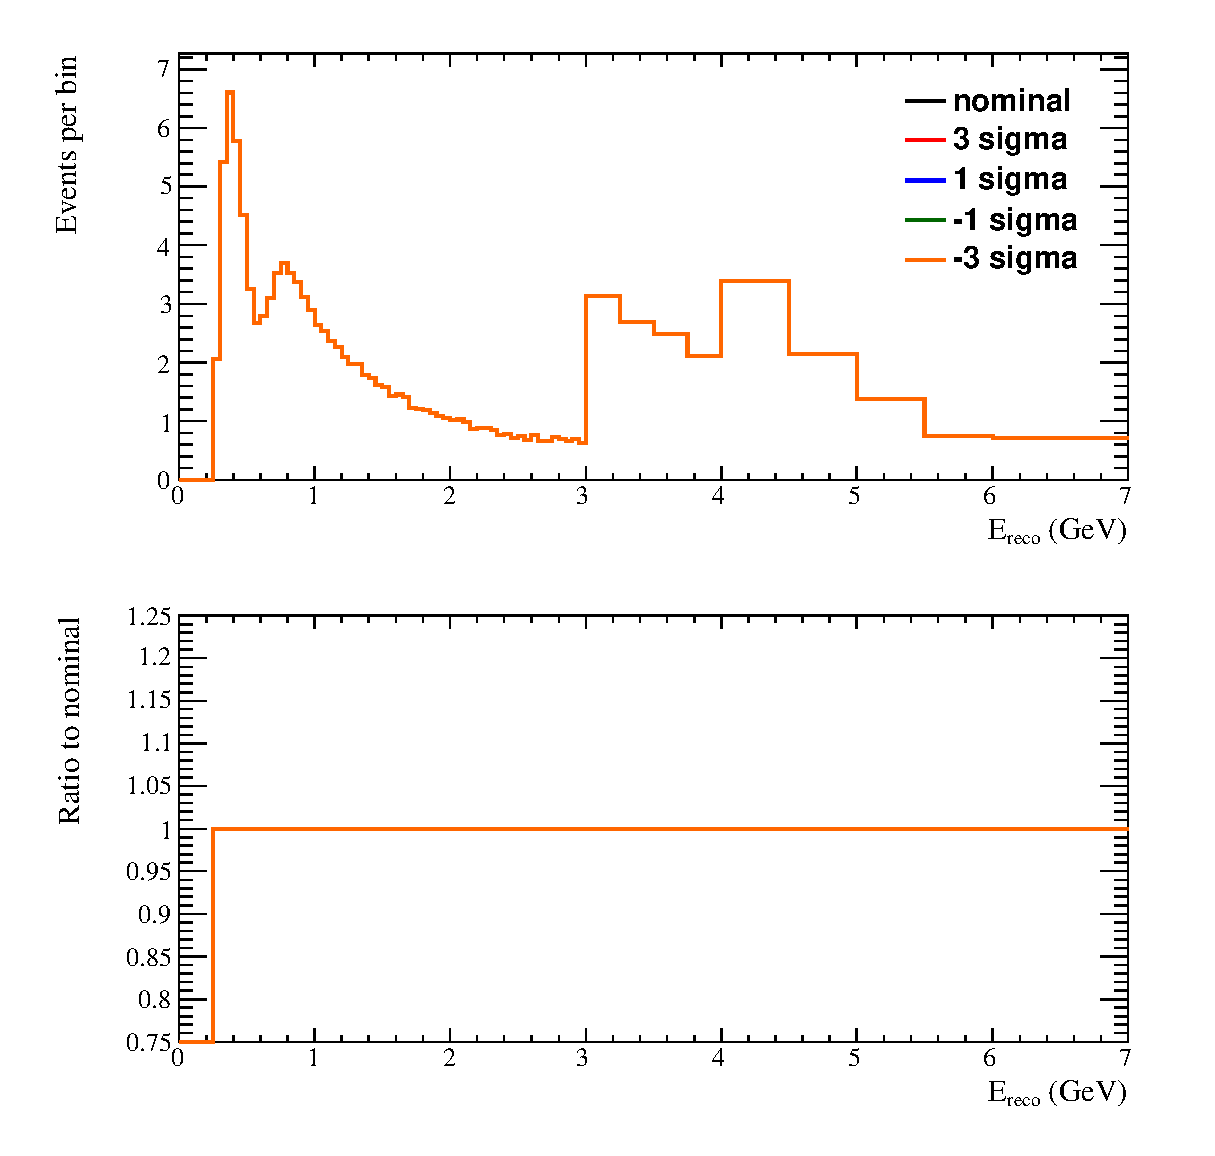
\includegraphics{../images/spectrum_tweaked/1sigma_oscillated/ereco_twk_dm12sq}}
\caption
{ Effect of $\Delta m^2_{21}$ for 3 flavour oscillations, using oscillation parameters:  $\sin^2\theta_{12} = $0.306; $\sin^2\theta_{13} = $0.0251; $\sin^2\theta_{23} = $0.5; $\delta_{CP} = $        0; $\Delta m^2_{21} = $    7.5e-05 eV$^2$/c$^4$; $|\Delta m^2_{32}| = $    0.0024 eV$^2$/c$^4$. }
\label{fig:osc_ereco_twk_dm12sq}
\end{center}
\end{figure}
\clearpage

\begin{figure}
\begin{center}
\resizebox{14cm}{!}{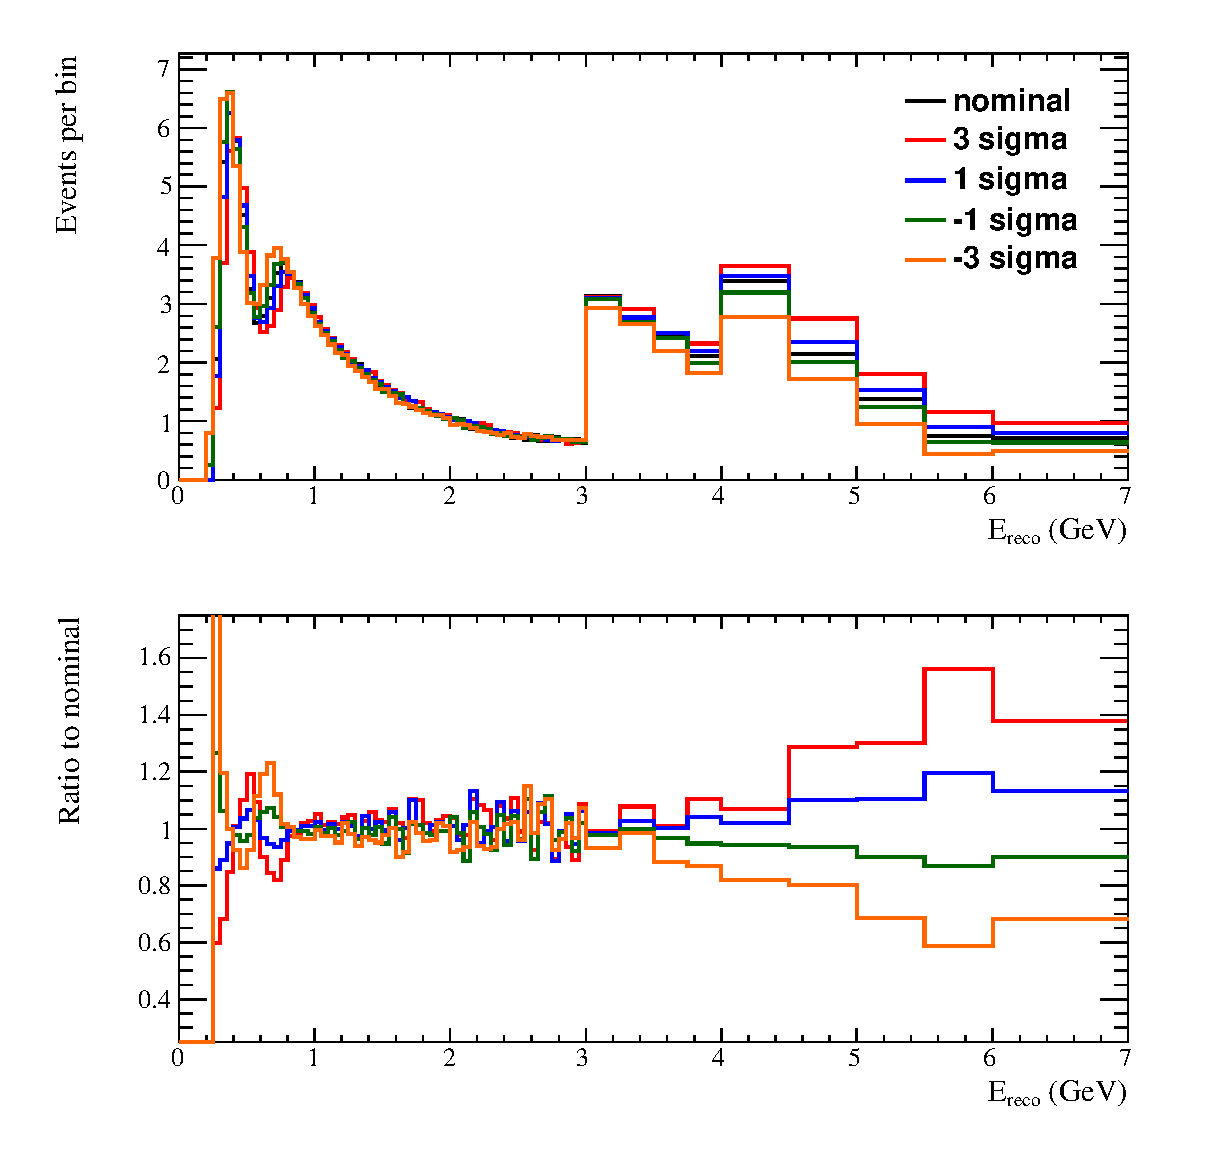
\includegraphics{../images/spectrum_tweaked/1sigma_oscillated/ereco_twk_f_sk_e_scale}}
\caption
{ Effect of $f_{E; r}^{SK}$   for 3 flavour oscillations, using oscillation parameters:  $\sin^2\theta_{12} = $0.306; $\sin^2\theta_{13} = $0.0251; $\sin^2\theta_{23} = $0.5; $\delta_{CP} = $        0; $\Delta m^2_{21} = $    7.5e-05 eV$^2$/c$^4$; $|\Delta m^2_{32}| = $    0.0024 eV$^2$/c$^4$. }
\label{fig:osc_ereco_twk_f_sk_e_scale}
\end{center}
\end{figure}
\clearpage

\begin{figure}
\begin{center}
\resizebox{14cm}{!}{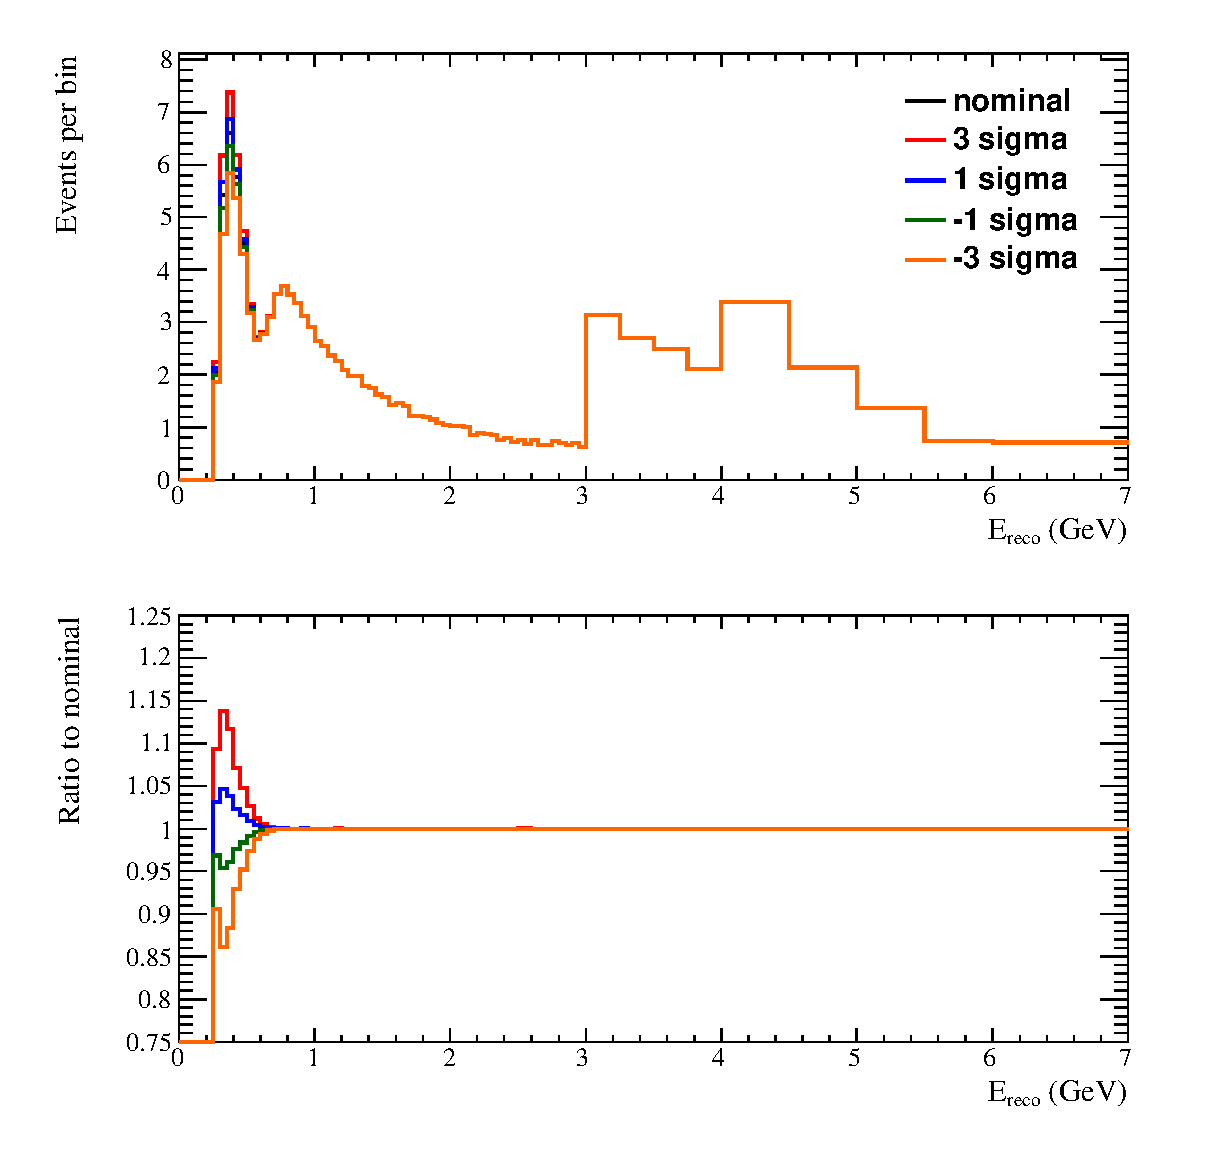
\includegraphics{../images/spectrum_tweaked/1sigma_oscillated/ereco_twk_f_banff00}}
\caption
{ Effect of $f_{0; t, r}^{banff}$ for 3 flavour oscillations, using oscillation parameters:  $\sin^2\theta_{12} = $0.306; $\sin^2\theta_{13} = $0.0251; $\sin^2\theta_{23} = $0.5; $\delta_{CP} = $        0; $\Delta m^2_{21} = $    7.5e-05 eV$^2$/c$^4$; $|\Delta m^2_{32}| = $    0.0024 eV$^2$/c$^4$. }
\label{fig:osc_ereco_twk_f_banff00}
\end{center}
\end{figure}
\clearpage

\begin{figure}
\begin{center}
\resizebox{14cm}{!}{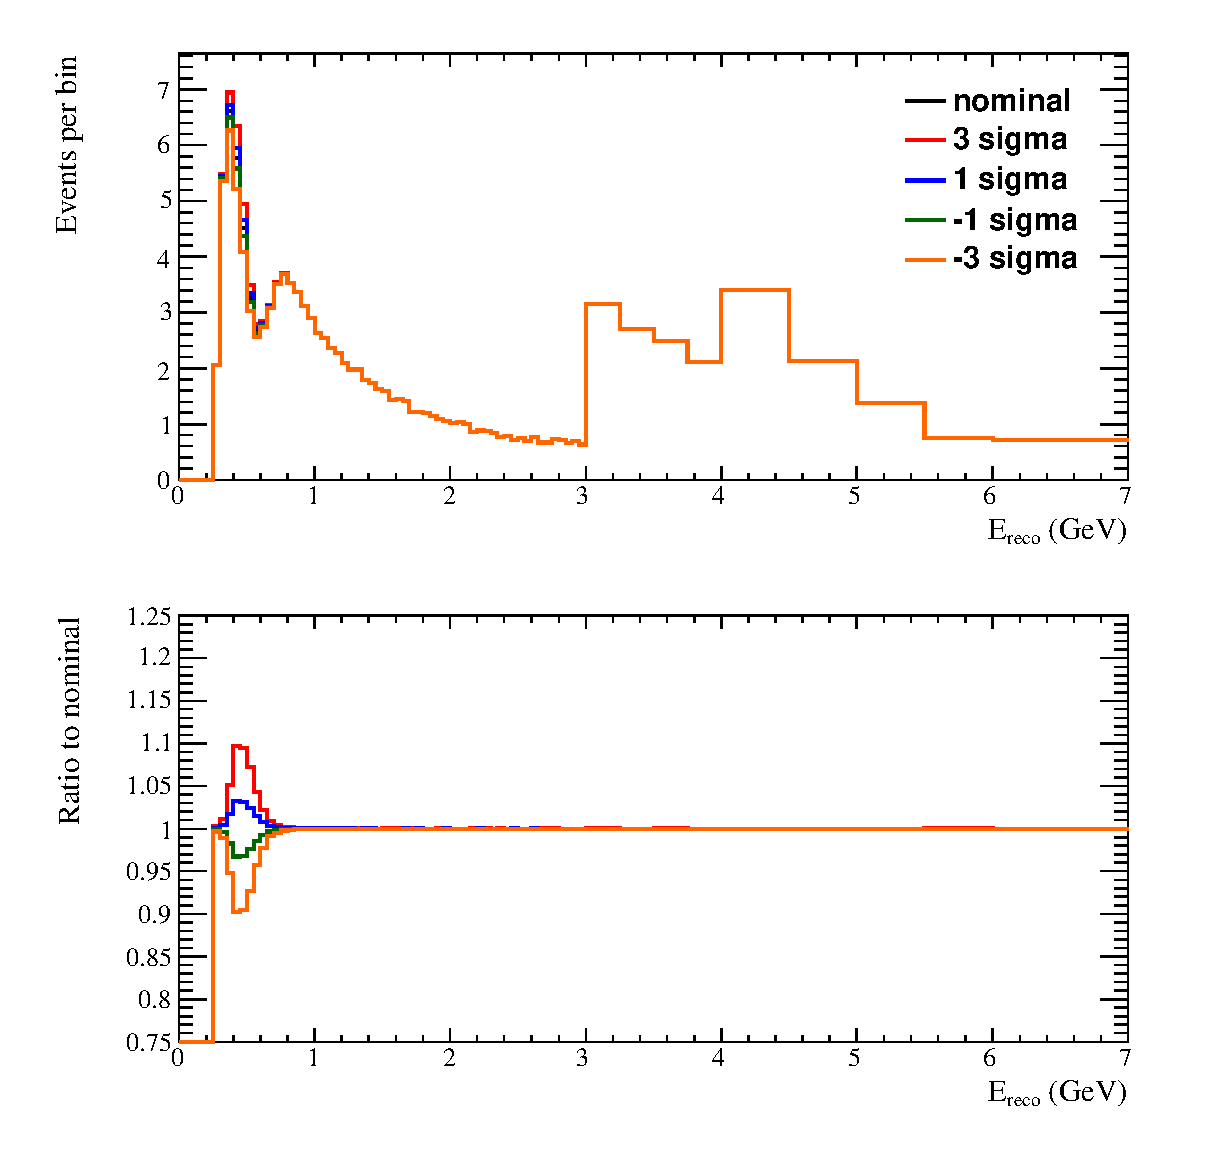
\includegraphics{../images/spectrum_tweaked/1sigma_oscillated/ereco_twk_f_banff01}}
\caption
{ Effect of $f_{1; t, r}^{banff}$ for 3 flavour oscillations, using oscillation parameters:  $\sin^2\theta_{12} = $0.306; $\sin^2\theta_{13} = $0.0251; $\sin^2\theta_{23} = $0.5; $\delta_{CP} = $        0; $\Delta m^2_{21} = $    7.5e-05 eV$^2$/c$^4$; $|\Delta m^2_{32}| = $    0.0024 eV$^2$/c$^4$. }
\label{fig:osc_ereco_twk_f_banff01}
\end{center}
\end{figure}
\clearpage

\begin{figure}
\begin{center}
\resizebox{14cm}{!}{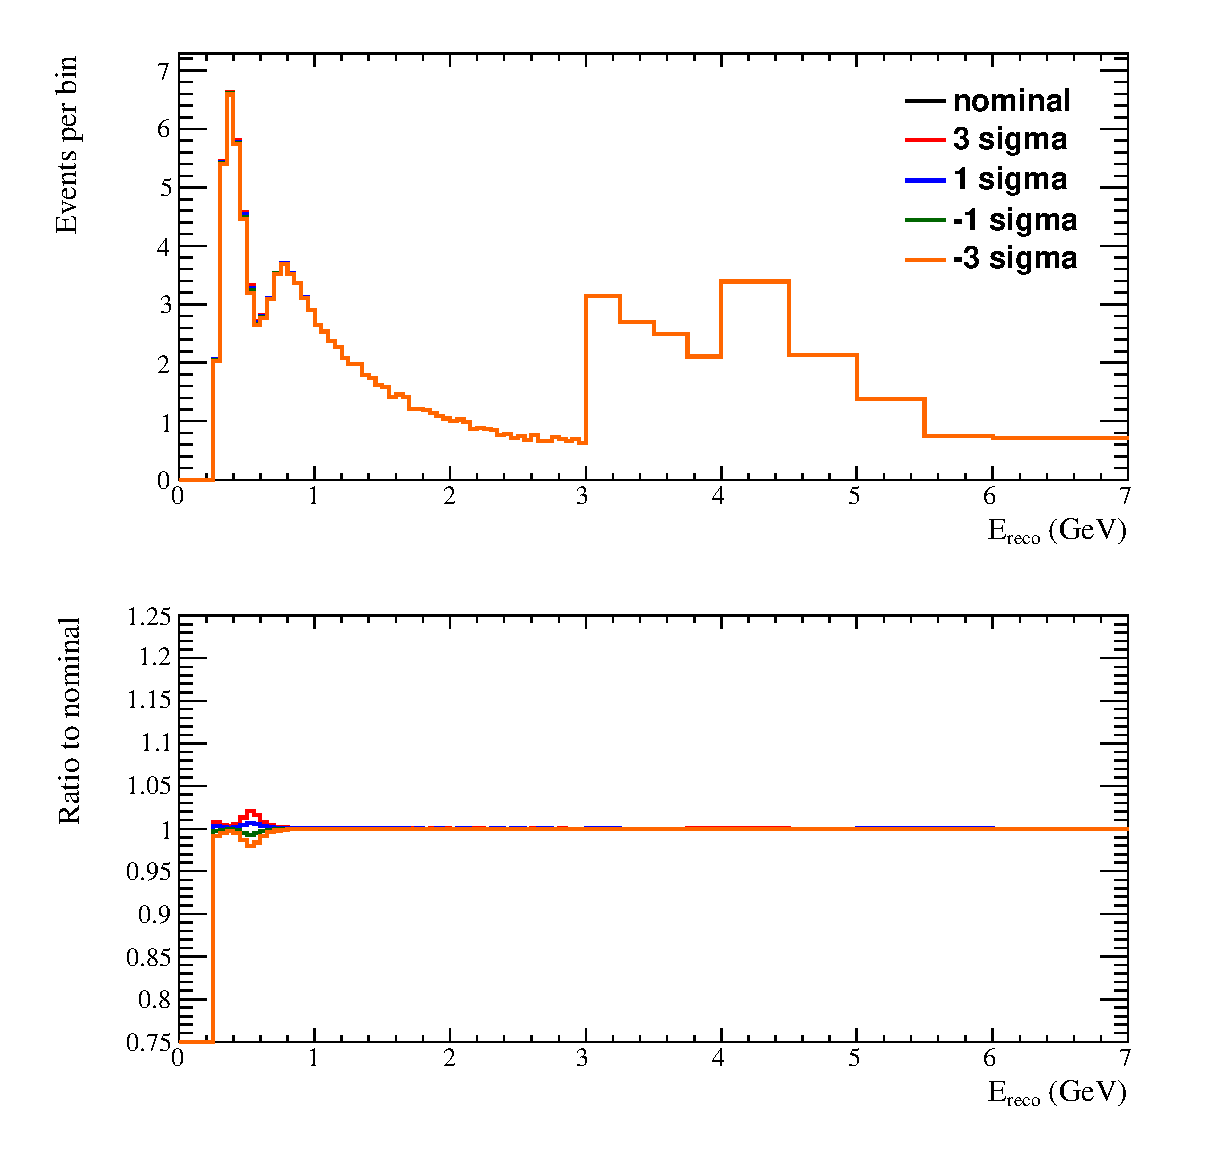
\includegraphics{../images/spectrum_tweaked/1sigma_oscillated/ereco_twk_f_banff02}}
\caption
{ Effect of $f_{2; t, r}^{banff}$ for 3 flavour oscillations, using oscillation parameters:  $\sin^2\theta_{12} = $0.306; $\sin^2\theta_{13} = $0.0251; $\sin^2\theta_{23} = $0.5; $\delta_{CP} = $        0; $\Delta m^2_{21} = $    7.5e-05 eV$^2$/c$^4$; $|\Delta m^2_{32}| = $    0.0024 eV$^2$/c$^4$. }
\label{fig:osc_ereco_twk_f_banff02}
\end{center}
\end{figure}
\clearpage

\begin{figure}
\begin{center}
\resizebox{14cm}{!}{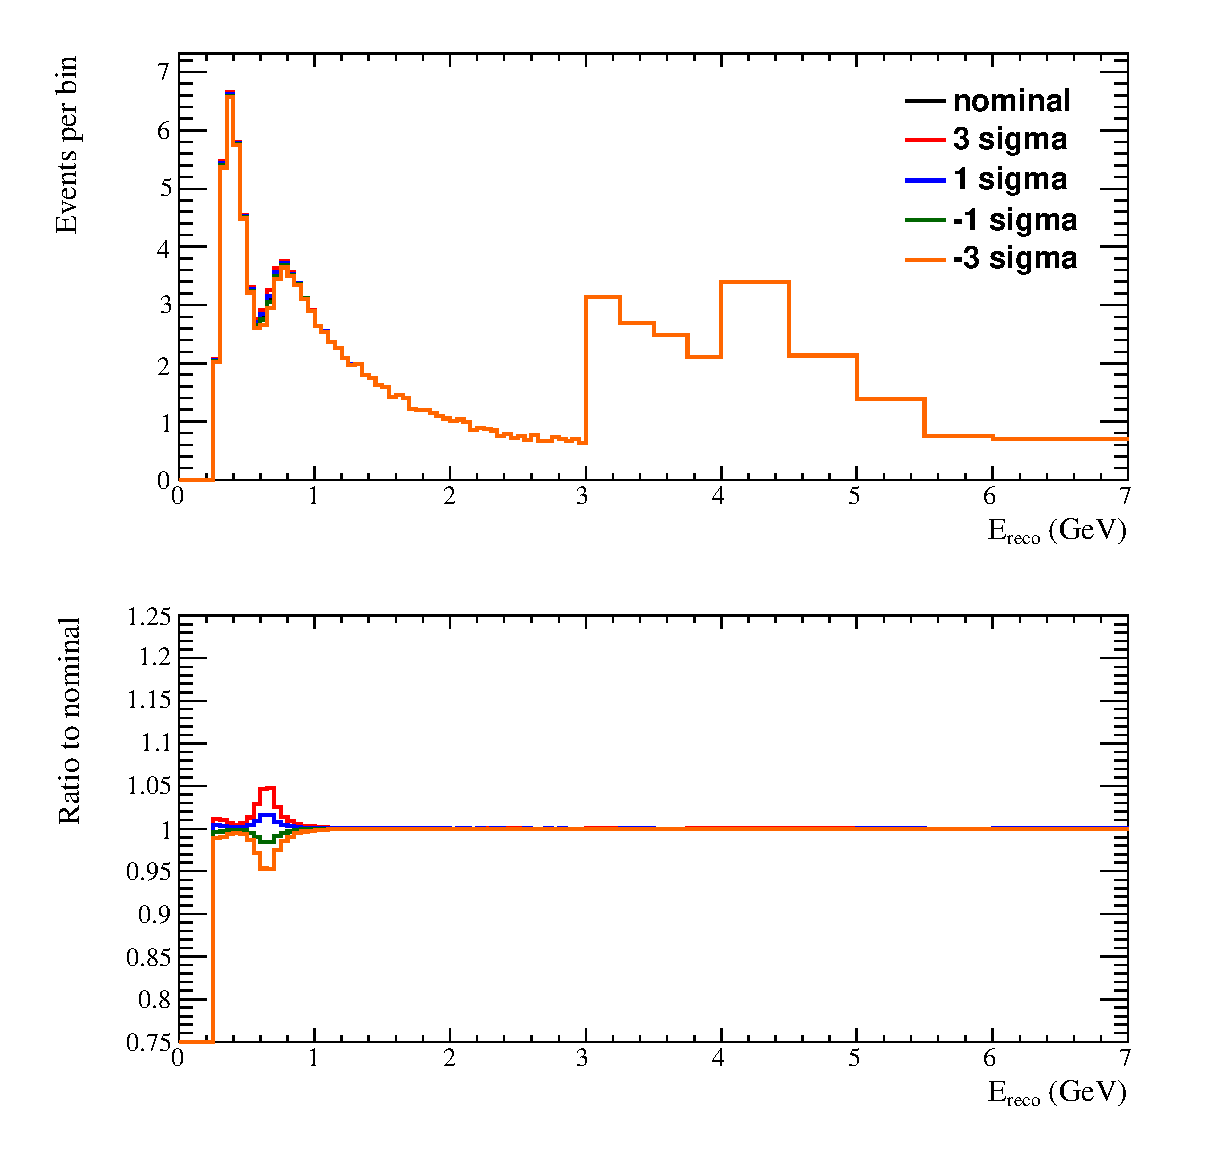
\includegraphics{../images/spectrum_tweaked/1sigma_oscillated/ereco_twk_f_banff03}}
\caption
{ Effect of $f_{3; t, r}^{banff}$ for 3 flavour oscillations, using oscillation parameters:  $\sin^2\theta_{12} = $0.306; $\sin^2\theta_{13} = $0.0251; $\sin^2\theta_{23} = $0.5; $\delta_{CP} = $        0; $\Delta m^2_{21} = $    7.5e-05 eV$^2$/c$^4$; $|\Delta m^2_{32}| = $    0.0024 eV$^2$/c$^4$. }
\label{fig:osc_ereco_twk_f_banff03}
\end{center}
\end{figure}
\clearpage

\begin{figure}
\begin{center}
\resizebox{14cm}{!}{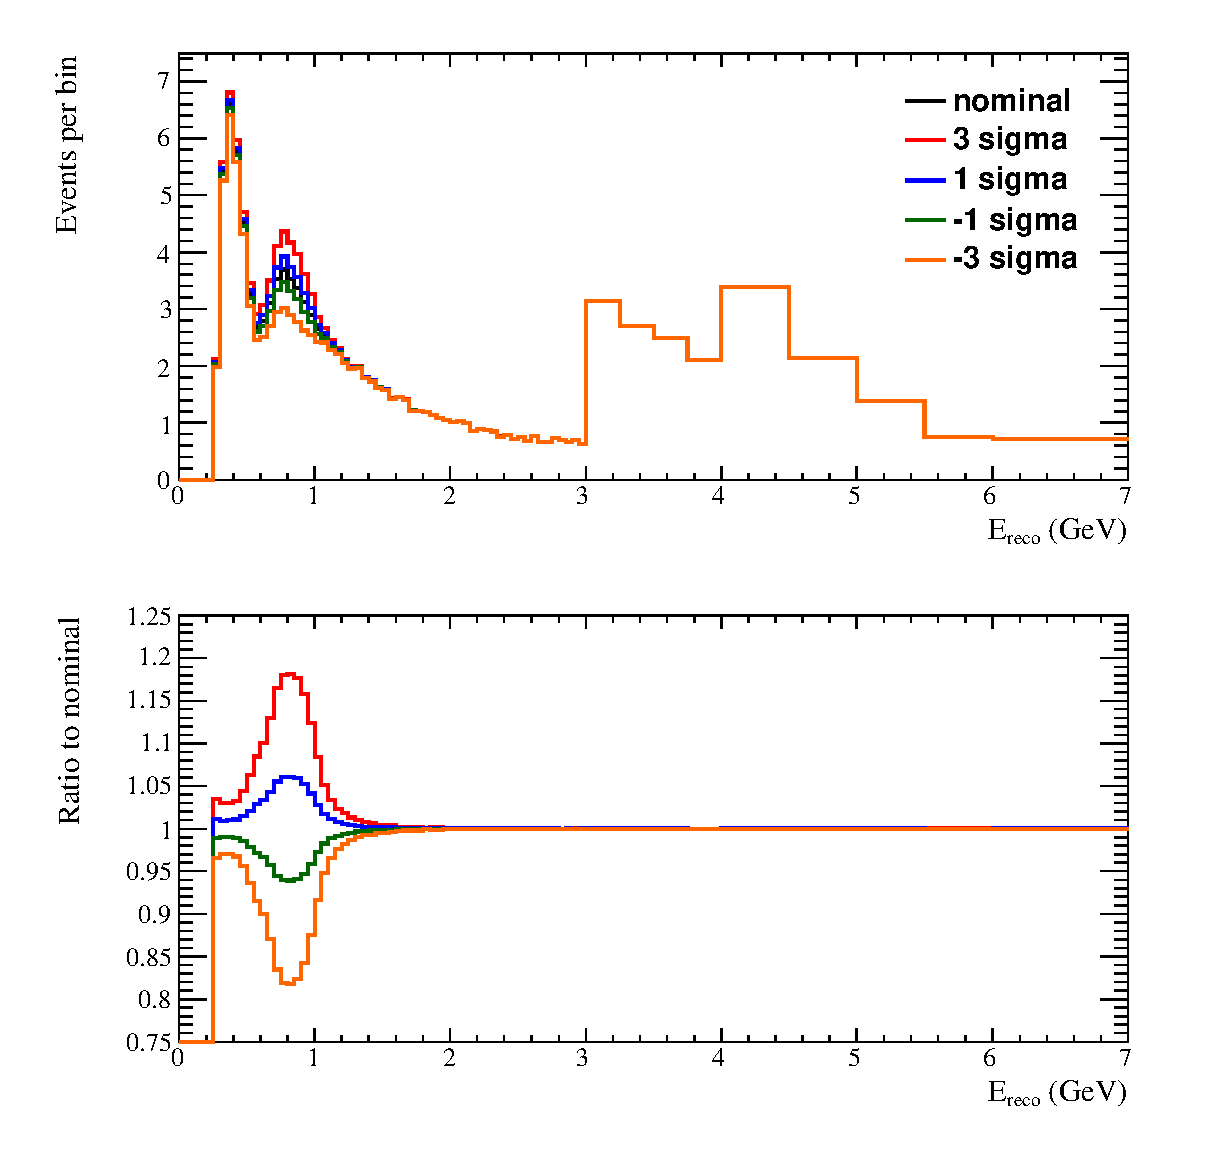
\includegraphics{../images/spectrum_tweaked/1sigma_oscillated/ereco_twk_f_banff04}}
\caption
{ Effect of $f_{4; t, r}^{banff}$ for 3 flavour oscillations, using oscillation parameters:  $\sin^2\theta_{12} = $0.306; $\sin^2\theta_{13} = $0.0251; $\sin^2\theta_{23} = $0.5; $\delta_{CP} = $        0; $\Delta m^2_{21} = $    7.5e-05 eV$^2$/c$^4$; $|\Delta m^2_{32}| = $    0.0024 eV$^2$/c$^4$. }
\label{fig:osc_ereco_twk_f_banff04}
\end{center}
\end{figure}
\clearpage

\begin{figure}
\begin{center}
\resizebox{14cm}{!}{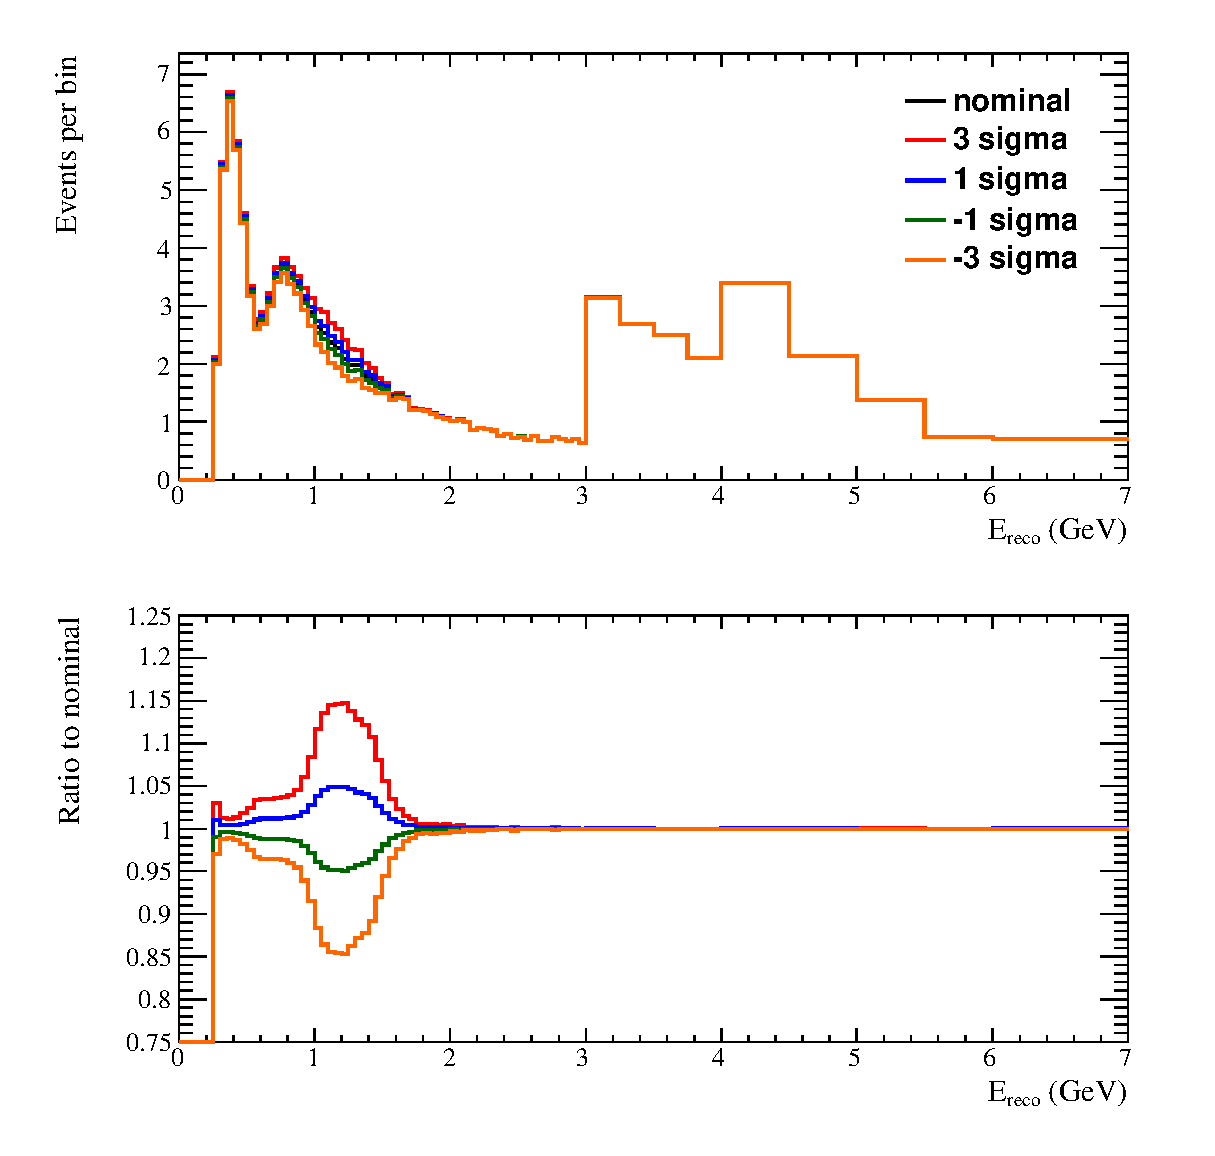
\includegraphics{../images/spectrum_tweaked/1sigma_oscillated/ereco_twk_f_banff05}}
\caption
{ Effect of $f_{5; t, r}^{banff}$ for 3 flavour oscillations, using oscillation parameters:  $\sin^2\theta_{12} = $0.306; $\sin^2\theta_{13} = $0.0251; $\sin^2\theta_{23} = $0.5; $\delta_{CP} = $        0; $\Delta m^2_{21} = $    7.5e-05 eV$^2$/c$^4$; $|\Delta m^2_{32}| = $    0.0024 eV$^2$/c$^4$. }
\label{fig:osc_ereco_twk_f_banff05}
\end{center}
\end{figure}
\clearpage

\begin{figure}
\begin{center}
\resizebox{14cm}{!}{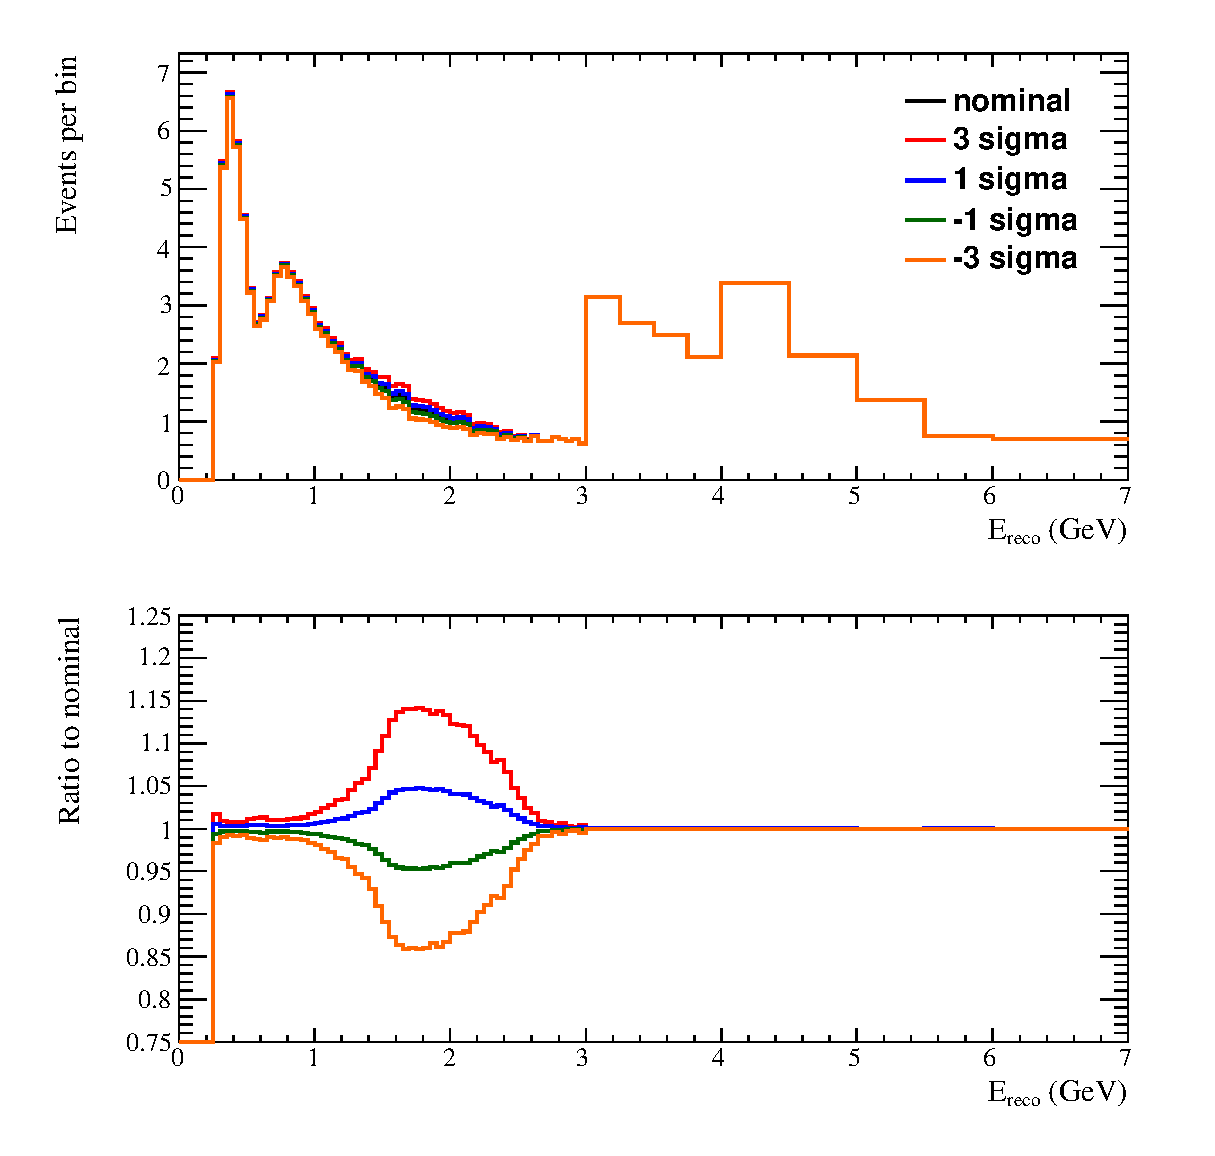
\includegraphics{../images/spectrum_tweaked/1sigma_oscillated/ereco_twk_f_banff06}}
\caption
{ Effect of $f_{6; t, r}^{banff}$ for 3 flavour oscillations, using oscillation parameters:  $\sin^2\theta_{12} = $0.306; $\sin^2\theta_{13} = $0.0251; $\sin^2\theta_{23} = $0.5; $\delta_{CP} = $        0; $\Delta m^2_{21} = $    7.5e-05 eV$^2$/c$^4$; $|\Delta m^2_{32}| = $    0.0024 eV$^2$/c$^4$. }
\label{fig:osc_ereco_twk_f_banff06}
\end{center}
\end{figure}
\clearpage

\begin{figure}
\begin{center}
\resizebox{14cm}{!}{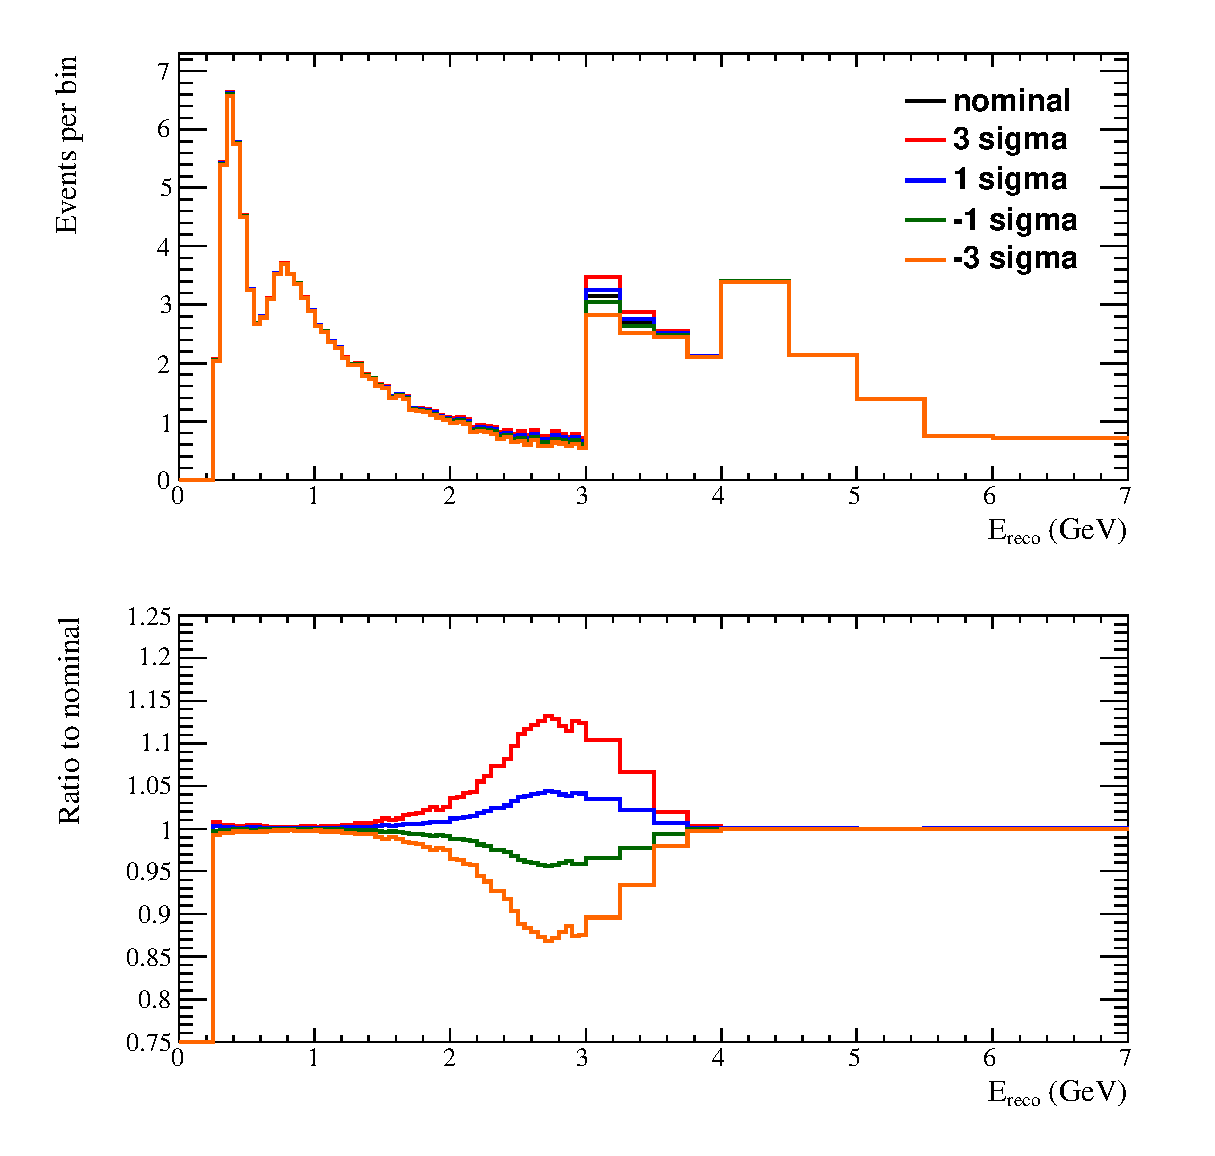
\includegraphics{../images/spectrum_tweaked/1sigma_oscillated/ereco_twk_f_banff07}}
\caption
{ Effect of $f_{7; t, r}^{banff}$ for 3 flavour oscillations, using oscillation parameters:  $\sin^2\theta_{12} = $0.306; $\sin^2\theta_{13} = $0.0251; $\sin^2\theta_{23} = $0.5; $\delta_{CP} = $        0; $\Delta m^2_{21} = $    7.5e-05 eV$^2$/c$^4$; $|\Delta m^2_{32}| = $    0.0024 eV$^2$/c$^4$. }
\label{fig:osc_ereco_twk_f_banff07}
\end{center}
\end{figure}
\clearpage

\begin{figure}
\begin{center}
\resizebox{14cm}{!}{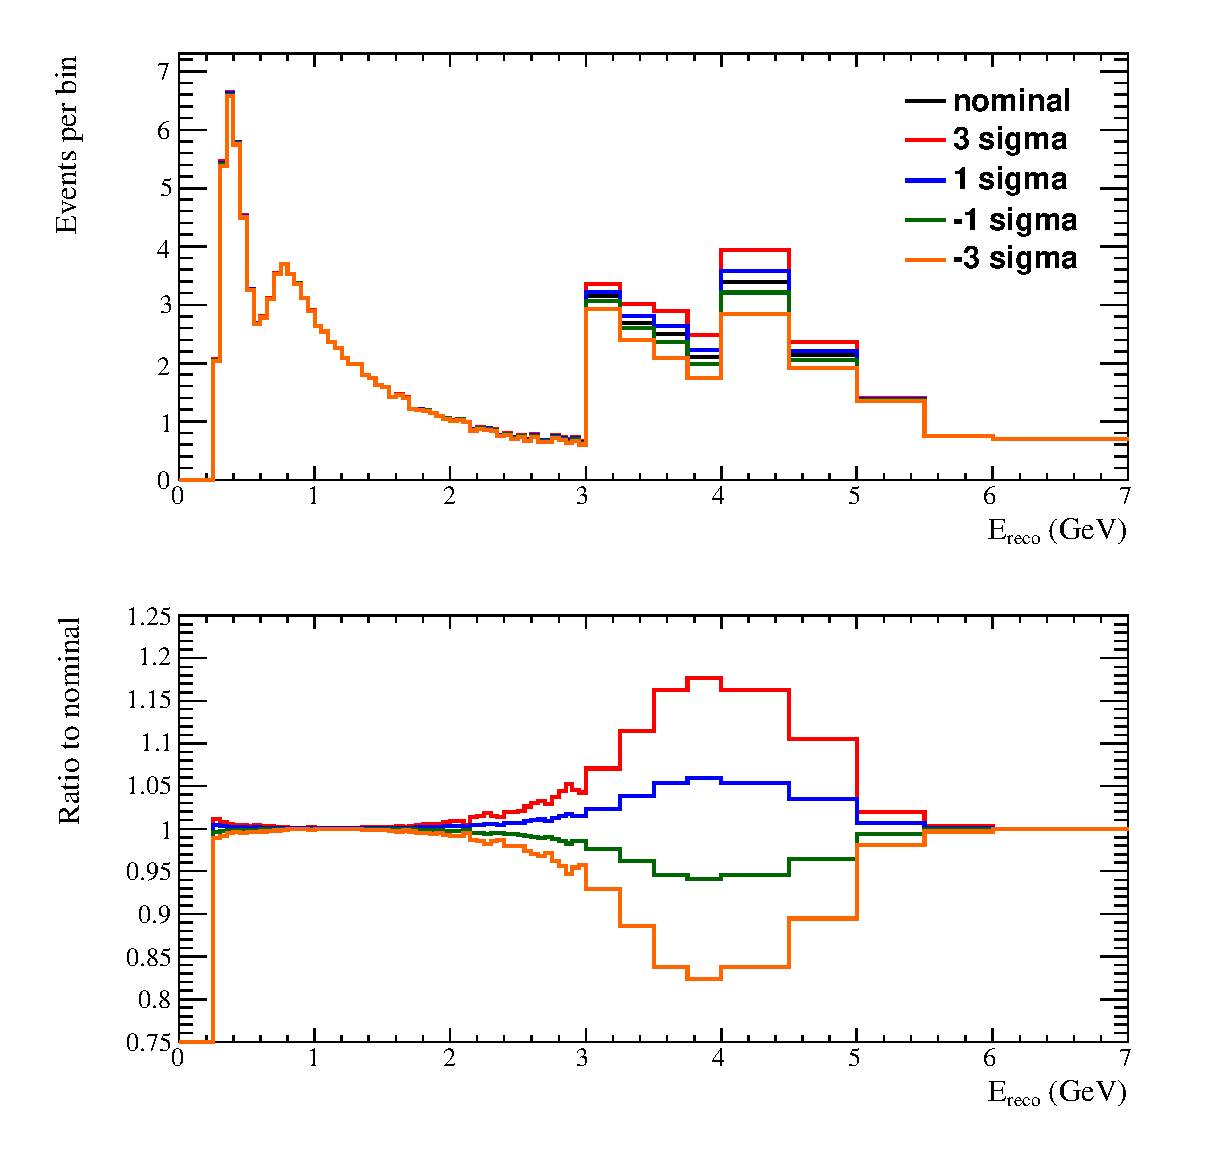
\includegraphics{../images/spectrum_tweaked/1sigma_oscillated/ereco_twk_f_banff08}}
\caption
{ Effect of $f_{8; t, r}^{banff}$ for 3 flavour oscillations, using oscillation parameters:  $\sin^2\theta_{12} = $0.306; $\sin^2\theta_{13} = $0.0251; $\sin^2\theta_{23} = $0.5; $\delta_{CP} = $        0; $\Delta m^2_{21} = $    7.5e-05 eV$^2$/c$^4$; $|\Delta m^2_{32}| = $    0.0024 eV$^2$/c$^4$. }
\label{fig:osc_ereco_twk_f_banff08}
\end{center}
\end{figure}
\clearpage

\begin{figure}
\begin{center}
\resizebox{14cm}{!}{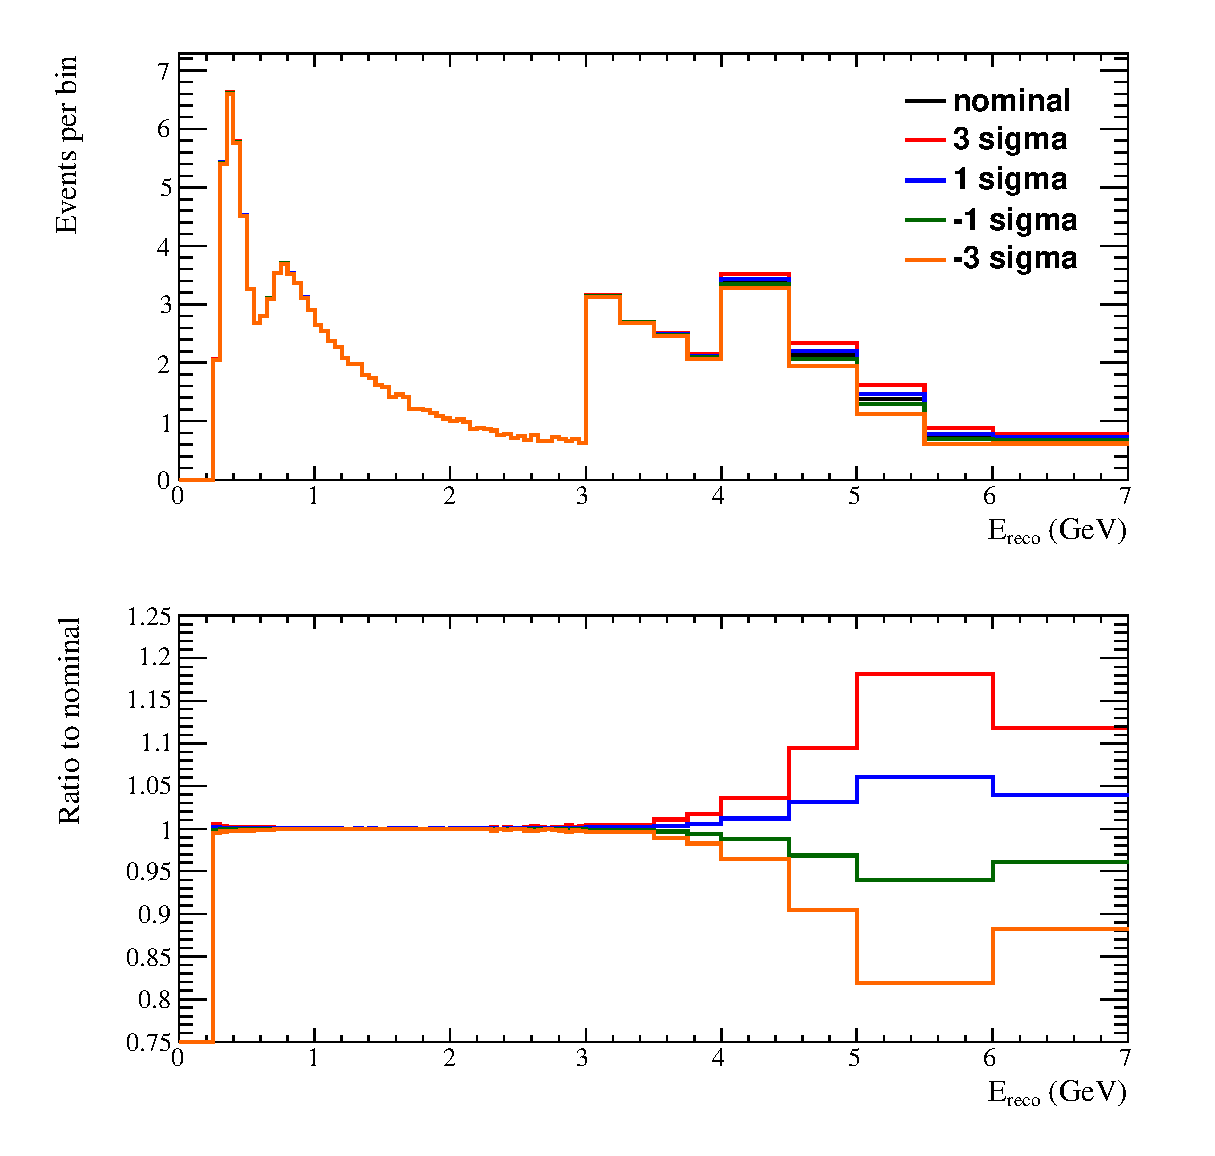
\includegraphics{../images/spectrum_tweaked/1sigma_oscillated/ereco_twk_f_banff09}}
\caption
{ Effect of $f_{9; t, r}^{banff}$ for 3 flavour oscillations, using oscillation parameters:  $\sin^2\theta_{12} = $0.306; $\sin^2\theta_{13} = $0.0251; $\sin^2\theta_{23} = $0.5; $\delta_{CP} = $        0; $\Delta m^2_{21} = $    7.5e-05 eV$^2$/c$^4$; $|\Delta m^2_{32}| = $    0.0024 eV$^2$/c$^4$. }
\label{fig:osc_ereco_twk_f_banff09}
\end{center}
\end{figure}
\clearpage

\begin{figure}
\begin{center}
\resizebox{14cm}{!}{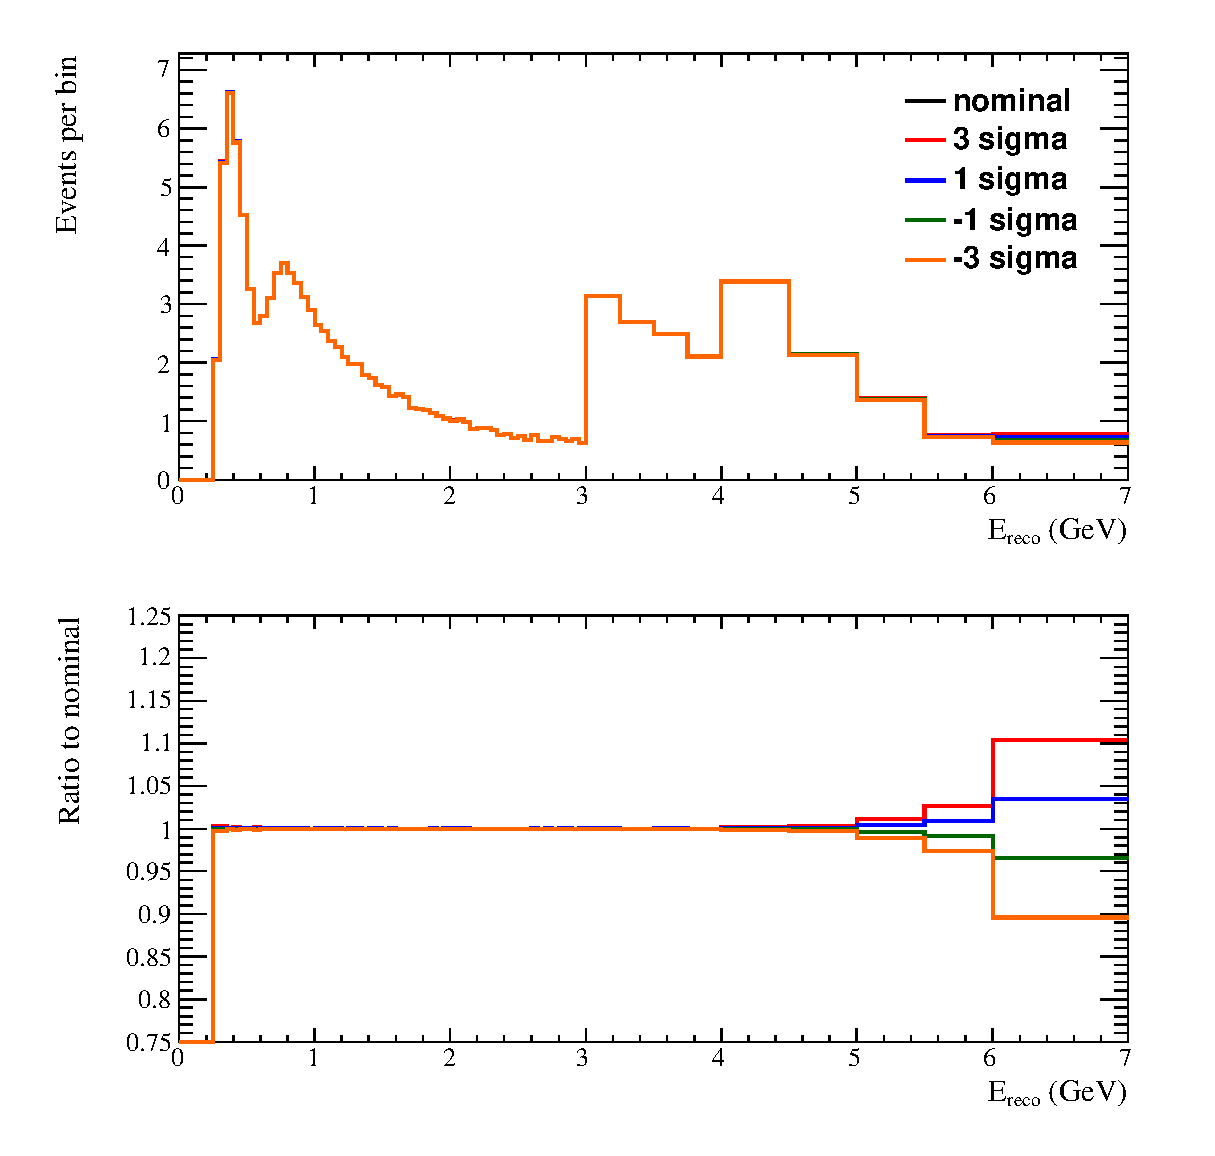
\includegraphics{../images/spectrum_tweaked/1sigma_oscillated/ereco_twk_f_banff10}}
\caption
{ Effect of $f_{10; t, r}^{banff}$ for 3 flavour oscillations, using oscillation parameters:  $\sin^2\theta_{12} = $0.306; $\sin^2\theta_{13} = $0.0251; $\sin^2\theta_{23} = $0.5; $\delta_{CP} = $        0; $\Delta m^2_{21} = $    7.5e-05 eV$^2$/c$^4$; $|\Delta m^2_{32}| = $    0.0024 eV$^2$/c$^4$. }
\label{fig:osc_ereco_twk_f_banff10}
\end{center}
\end{figure}
\clearpage

\begin{figure}
\begin{center}
\resizebox{14cm}{!}{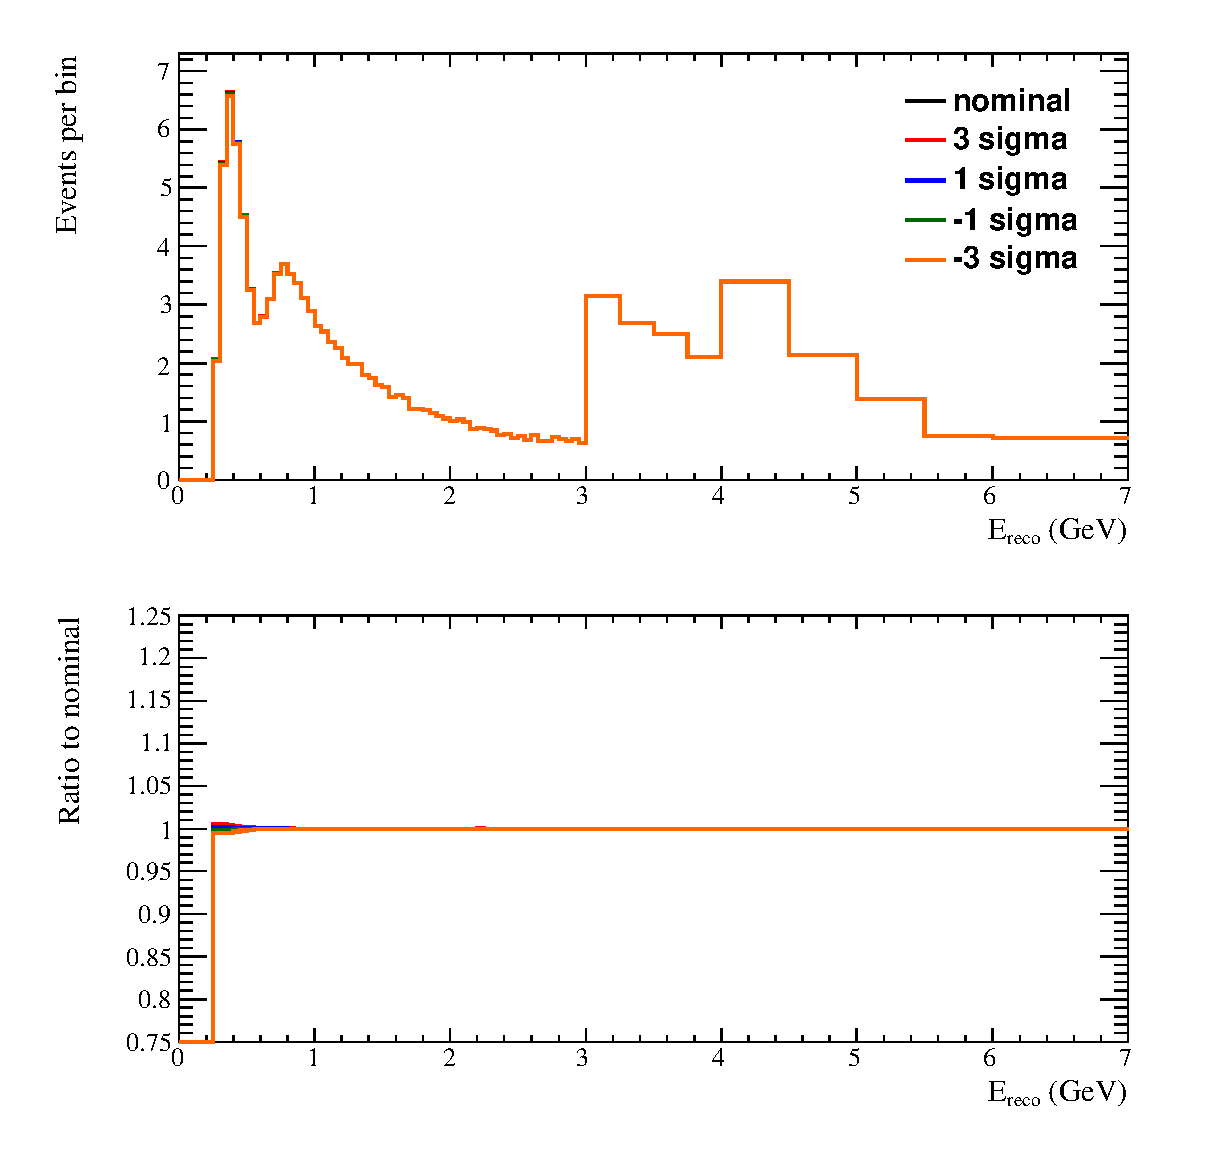
\includegraphics{../images/spectrum_tweaked/1sigma_oscillated/ereco_twk_f_banff11}}
\caption
{ Effect of $f_{11; t, r}^{banff}$ for 3 flavour oscillations, using oscillation parameters:  $\sin^2\theta_{12} = $0.306; $\sin^2\theta_{13} = $0.0251; $\sin^2\theta_{23} = $0.5; $\delta_{CP} = $        0; $\Delta m^2_{21} = $    7.5e-05 eV$^2$/c$^4$; $|\Delta m^2_{32}| = $    0.0024 eV$^2$/c$^4$. }
\label{fig:osc_ereco_twk_f_banff11}
\end{center}
\end{figure}
\clearpage

\begin{figure}
\begin{center}
\resizebox{14cm}{!}{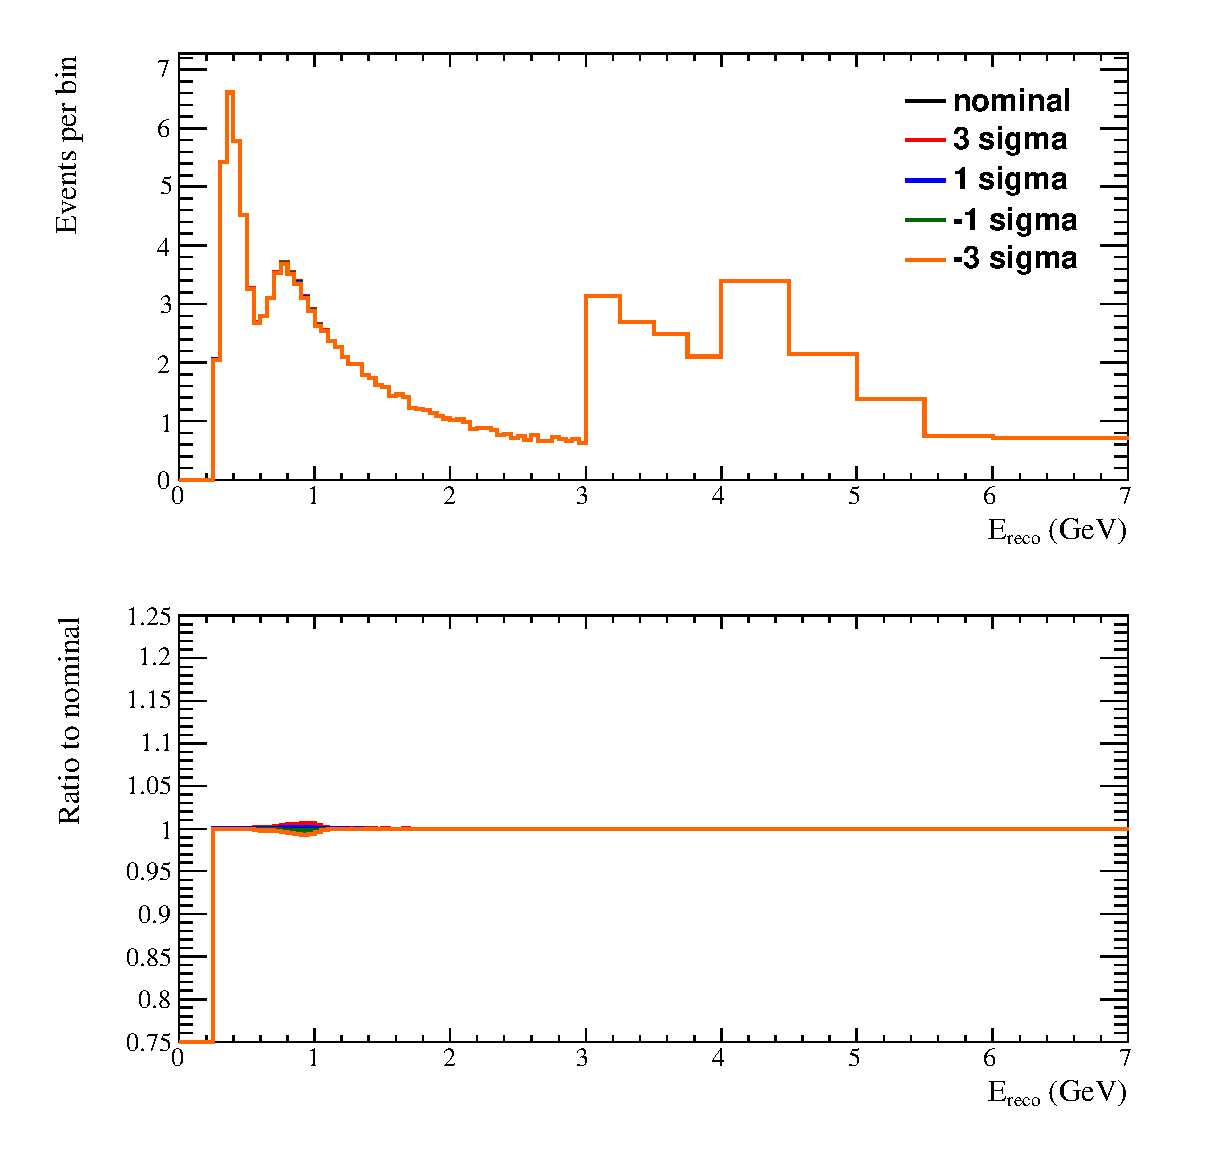
\includegraphics{../images/spectrum_tweaked/1sigma_oscillated/ereco_twk_f_banff12}}
\caption
{ Effect of $f_{12; t, r}^{banff}$ for 3 flavour oscillations, using oscillation parameters:  $\sin^2\theta_{12} = $0.306; $\sin^2\theta_{13} = $0.0251; $\sin^2\theta_{23} = $0.5; $\delta_{CP} = $        0; $\Delta m^2_{21} = $    7.5e-05 eV$^2$/c$^4$; $|\Delta m^2_{32}| = $    0.0024 eV$^2$/c$^4$. }
\label{fig:osc_ereco_twk_f_banff12}
\end{center}
\end{figure}
\clearpage

\begin{figure}
\begin{center}
\resizebox{14cm}{!}{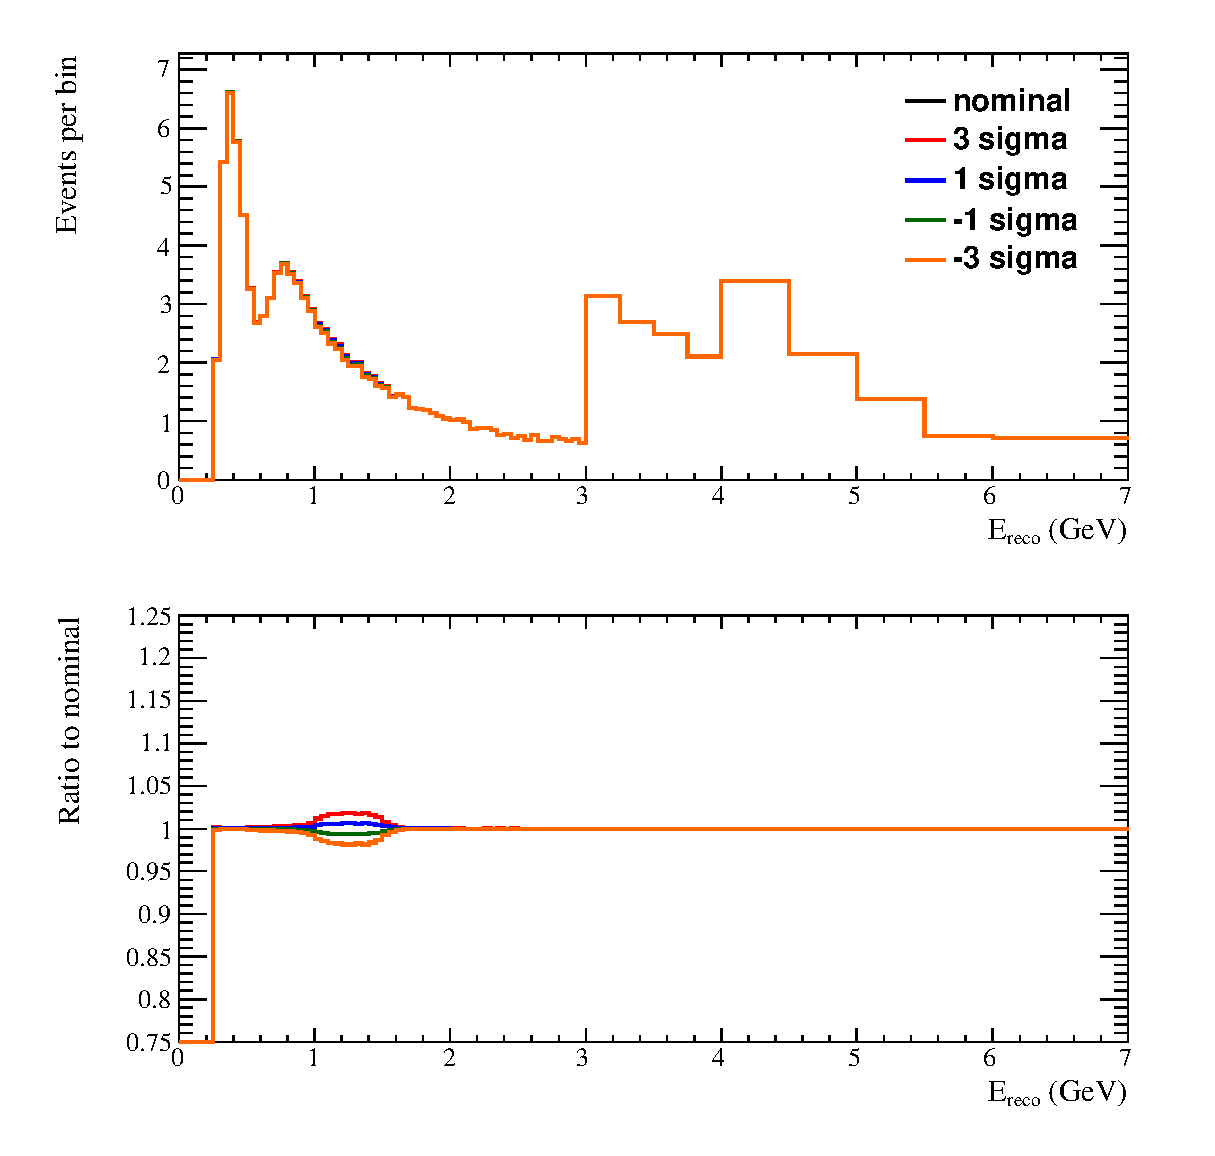
\includegraphics{../images/spectrum_tweaked/1sigma_oscillated/ereco_twk_f_banff13}}
\caption
{ Effect of $f_{13; t, r}^{banff}$ for 3 flavour oscillations, using oscillation parameters:  $\sin^2\theta_{12} = $0.306; $\sin^2\theta_{13} = $0.0251; $\sin^2\theta_{23} = $0.5; $\delta_{CP} = $        0; $\Delta m^2_{21} = $    7.5e-05 eV$^2$/c$^4$; $|\Delta m^2_{32}| = $    0.0024 eV$^2$/c$^4$. }
\label{fig:osc_ereco_twk_f_banff13}
\end{center}
\end{figure}
\clearpage

\begin{figure}
\begin{center}
\resizebox{14cm}{!}{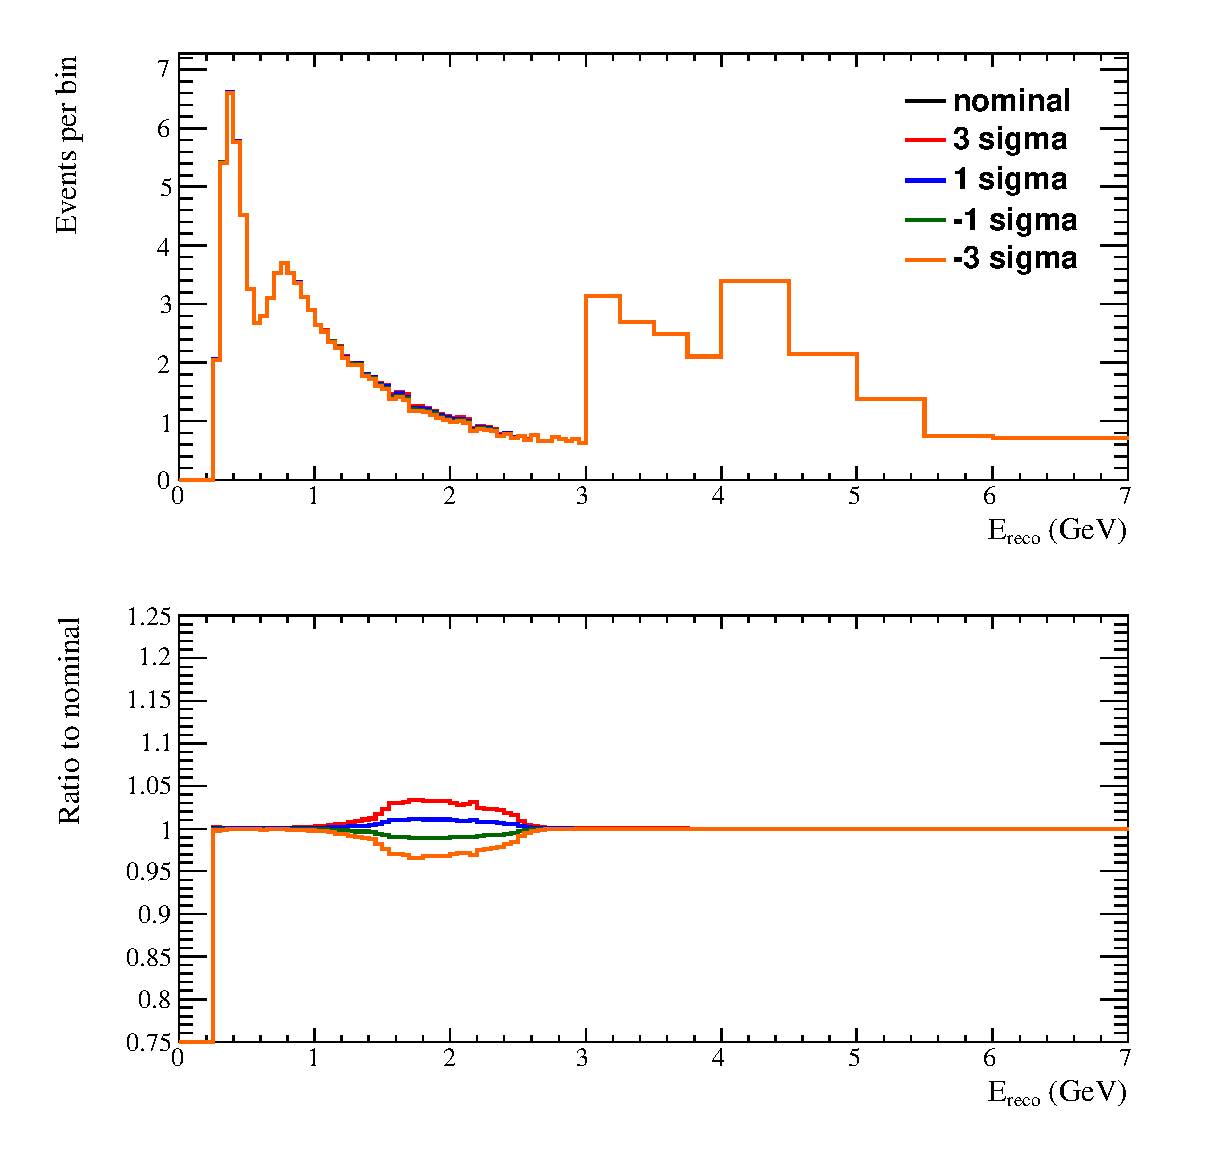
\includegraphics{../images/spectrum_tweaked/1sigma_oscillated/ereco_twk_f_banff14}}
\caption
{ Effect of $f_{14; t, r}^{banff}$ for 3 flavour oscillations, using oscillation parameters:  $\sin^2\theta_{12} = $0.306; $\sin^2\theta_{13} = $0.0251; $\sin^2\theta_{23} = $0.5; $\delta_{CP} = $        0; $\Delta m^2_{21} = $    7.5e-05 eV$^2$/c$^4$; $|\Delta m^2_{32}| = $    0.0024 eV$^2$/c$^4$. }
\label{fig:osc_ereco_twk_f_banff14}
\end{center}
\end{figure}
\clearpage

\begin{figure}
\begin{center}
\resizebox{14cm}{!}{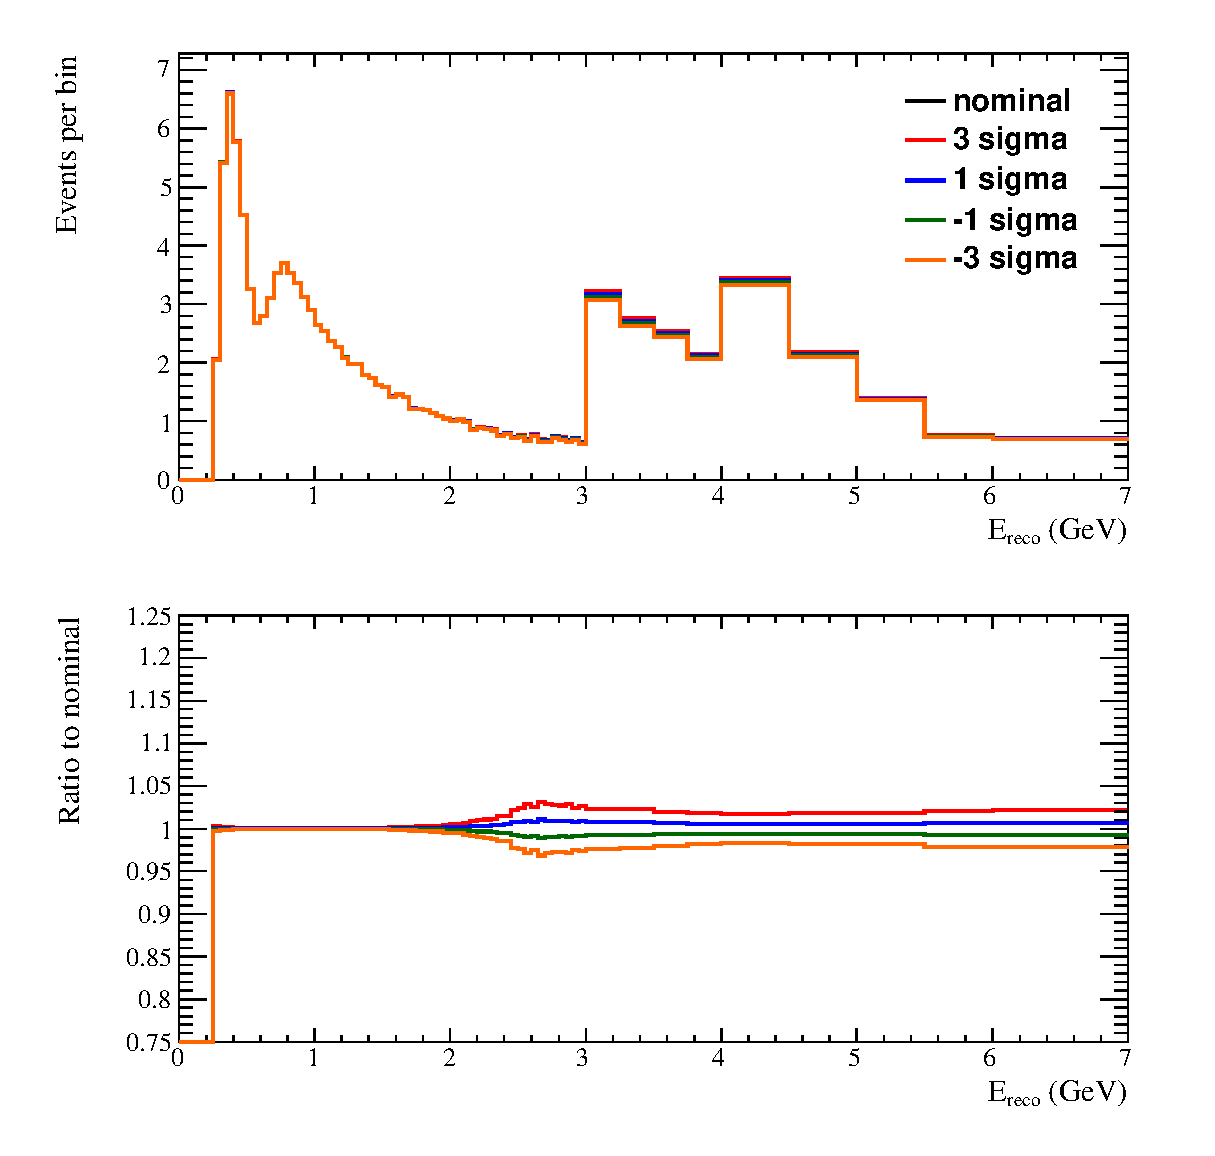
\includegraphics{../images/spectrum_tweaked/1sigma_oscillated/ereco_twk_f_banff15}}
\caption
{ Effect of $f_{15; t, r}^{banff}$ for 3 flavour oscillations, using oscillation parameters:  $\sin^2\theta_{12} = $0.306; $\sin^2\theta_{13} = $0.0251; $\sin^2\theta_{23} = $0.5; $\delta_{CP} = $        0; $\Delta m^2_{21} = $    7.5e-05 eV$^2$/c$^4$; $|\Delta m^2_{32}| = $    0.0024 eV$^2$/c$^4$. }
\label{fig:osc_ereco_twk_f_banff15}
\end{center}
\end{figure}
\clearpage

\begin{figure}
\begin{center}
\resizebox{14cm}{!}{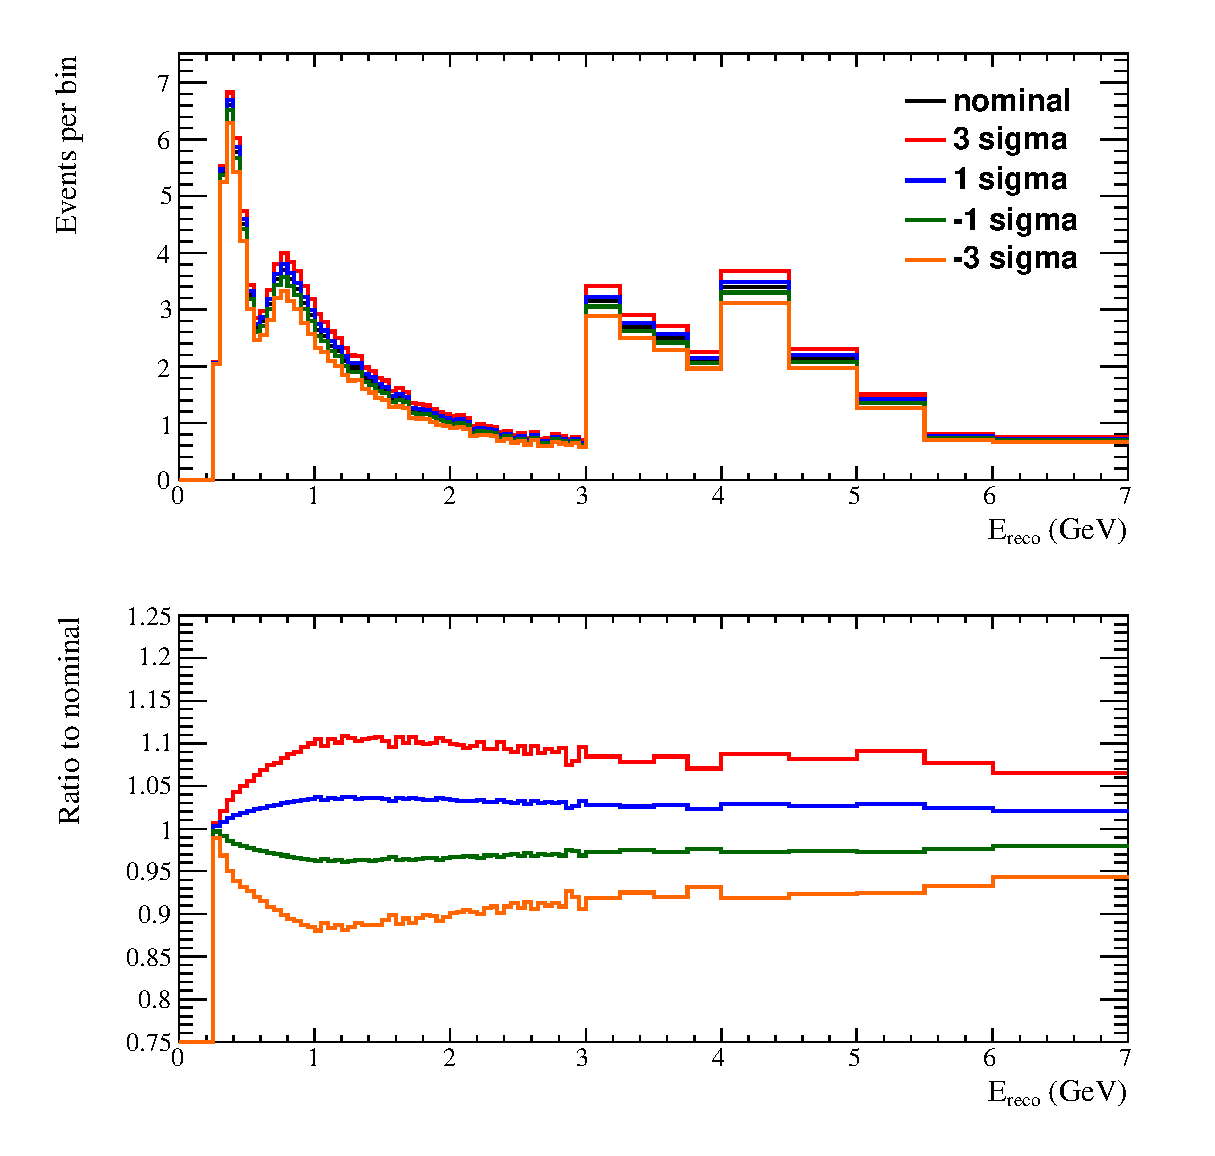
\includegraphics{../images/spectrum_tweaked/1sigma_oscillated/ereco_twk_f_banffmaqe}}
\caption
{ Effect of $f_{16; t, r}^{banff}$ for 3 flavour oscillations, using oscillation parameters:  $\sin^2\theta_{12} = $0.306; $\sin^2\theta_{13} = $0.0251; $\sin^2\theta_{23} = $0.5; $\delta_{CP} = $        0; $\Delta m^2_{21} = $    7.5e-05 eV$^2$/c$^4$; $|\Delta m^2_{32}| = $    0.0024 eV$^2$/c$^4$. }
\label{fig:osc_ereco_twk_f_banffmaqe}
\end{center}
\end{figure}
\clearpage

\begin{figure}
\begin{center}
\resizebox{14cm}{!}{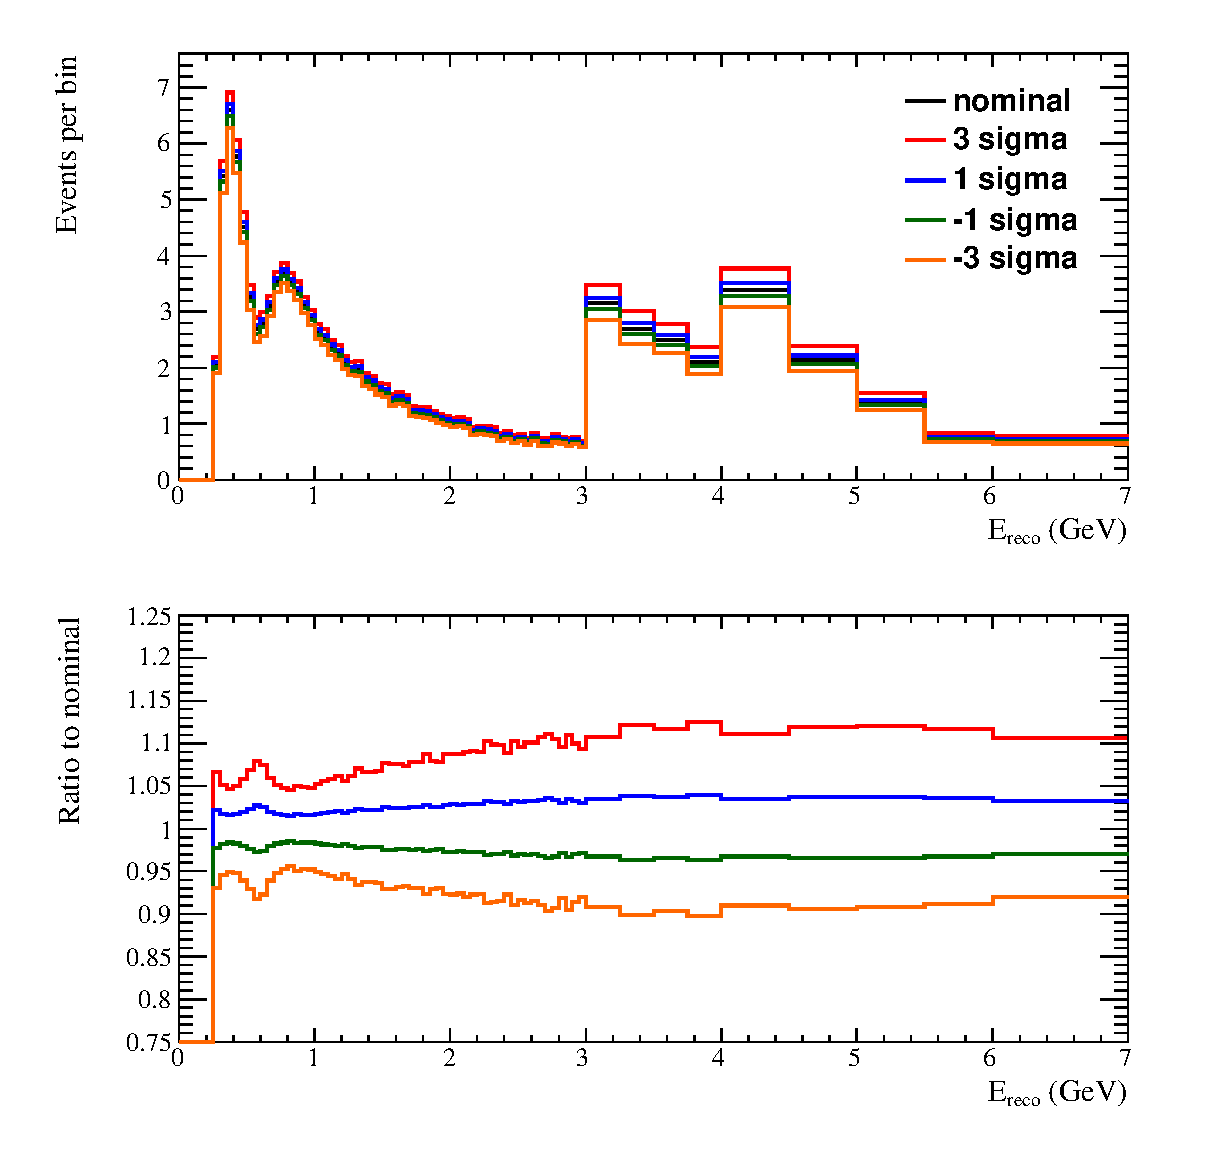
\includegraphics{../images/spectrum_tweaked/1sigma_oscillated/ereco_twk_f_banffmares}}
\caption
{ Effect of $f_{17; t, r}^{banff}$ for 3 flavour oscillations, using oscillation parameters:  $\sin^2\theta_{12} = $0.306; $\sin^2\theta_{13} = $0.0251; $\sin^2\theta_{23} = $0.5; $\delta_{CP} = $        0; $\Delta m^2_{21} = $    7.5e-05 eV$^2$/c$^4$; $|\Delta m^2_{32}| = $    0.0024 eV$^2$/c$^4$. }
\label{fig:osc_ereco_twk_f_banffmares}
\end{center}
\end{figure}
\clearpage

\begin{figure}
\begin{center}
\resizebox{14cm}{!}{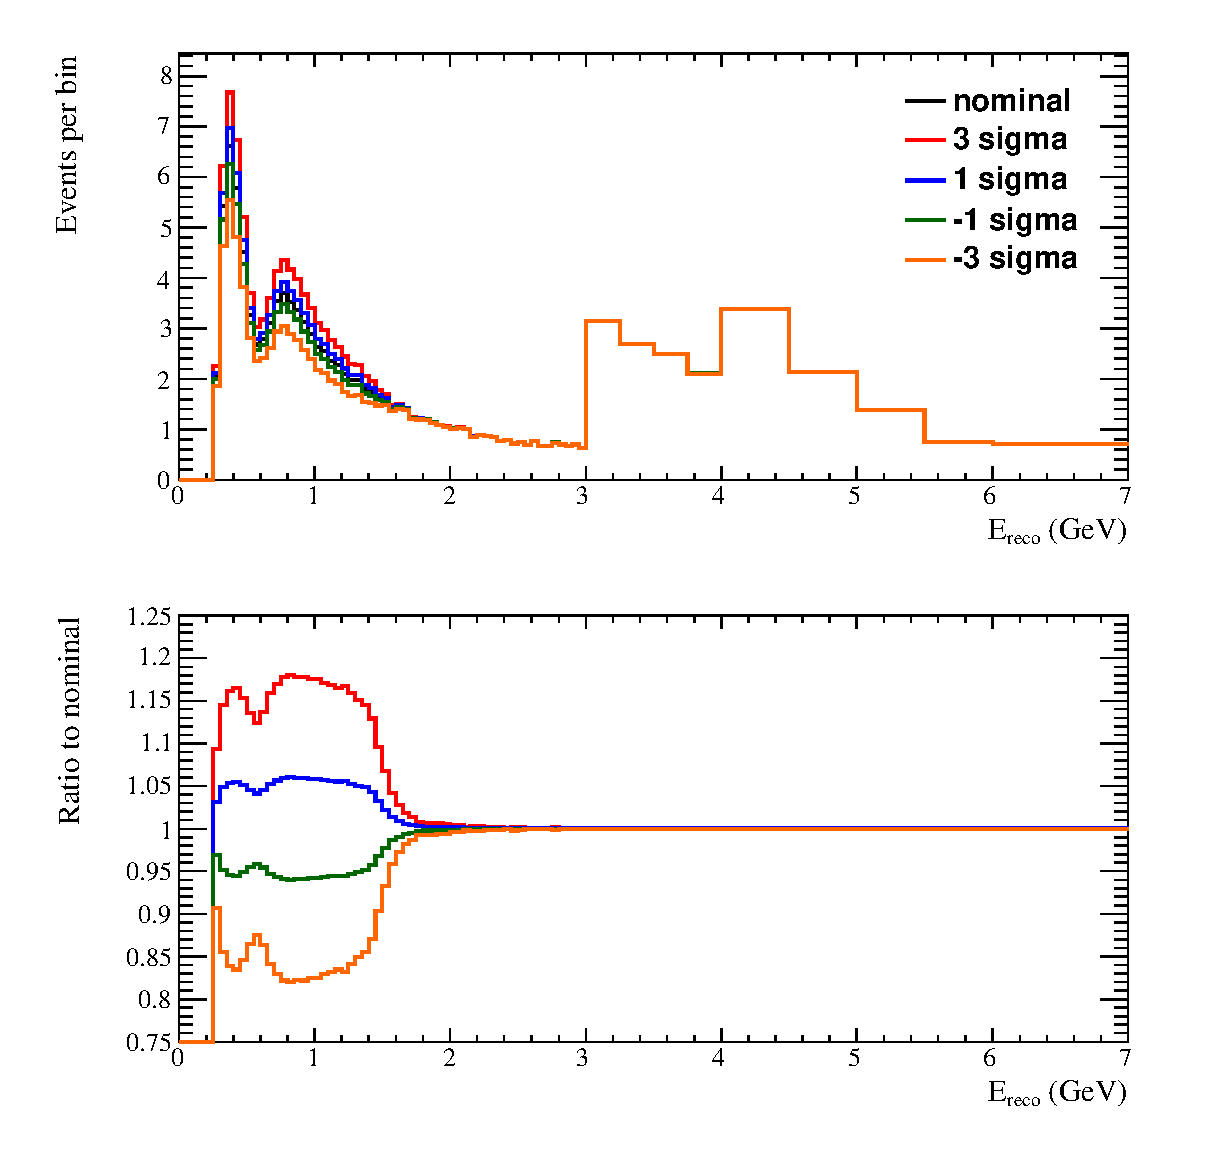
\includegraphics{../images/spectrum_tweaked/1sigma_oscillated/ereco_twk_f_banffccqee0}}
\caption
{ Effect of $f_{18; t, r}^{banff}$ for 3 flavour oscillations, using oscillation parameters:  $\sin^2\theta_{12} = $0.306; $\sin^2\theta_{13} = $0.0251; $\sin^2\theta_{23} = $0.5; $\delta_{CP} = $        0; $\Delta m^2_{21} = $    7.5e-05 eV$^2$/c$^4$; $|\Delta m^2_{32}| = $    0.0024 eV$^2$/c$^4$. }
\label{fig:osc_ereco_twk_f_banffccqee0}
\end{center}
\end{figure}
\clearpage

\begin{figure}
\begin{center}
\resizebox{14cm}{!}{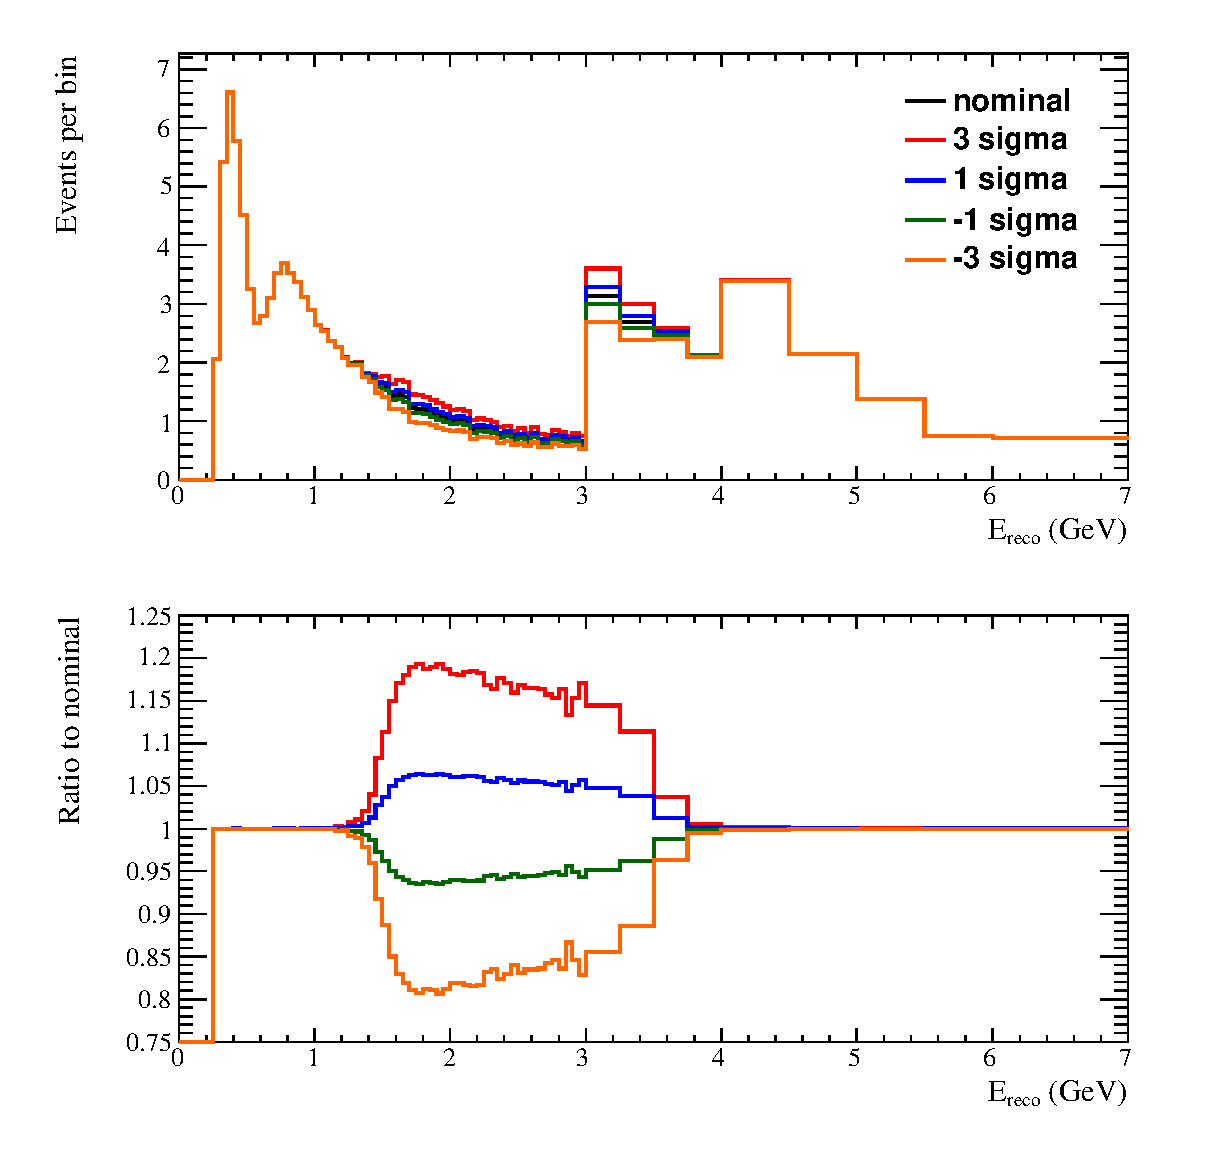
\includegraphics{../images/spectrum_tweaked/1sigma_oscillated/ereco_twk_f_banffccqee1}}
\caption
{ Effect of $f_{19; t, r}^{banff}$ for 3 flavour oscillations, using oscillation parameters:  $\sin^2\theta_{12} = $0.306; $\sin^2\theta_{13} = $0.0251; $\sin^2\theta_{23} = $0.5; $\delta_{CP} = $        0; $\Delta m^2_{21} = $    7.5e-05 eV$^2$/c$^4$; $|\Delta m^2_{32}| = $    0.0024 eV$^2$/c$^4$. }
\label{fig:osc_ereco_twk_f_banffccqee1}
\end{center}
\end{figure}
\clearpage

\begin{figure}
\begin{center}
\resizebox{14cm}{!}{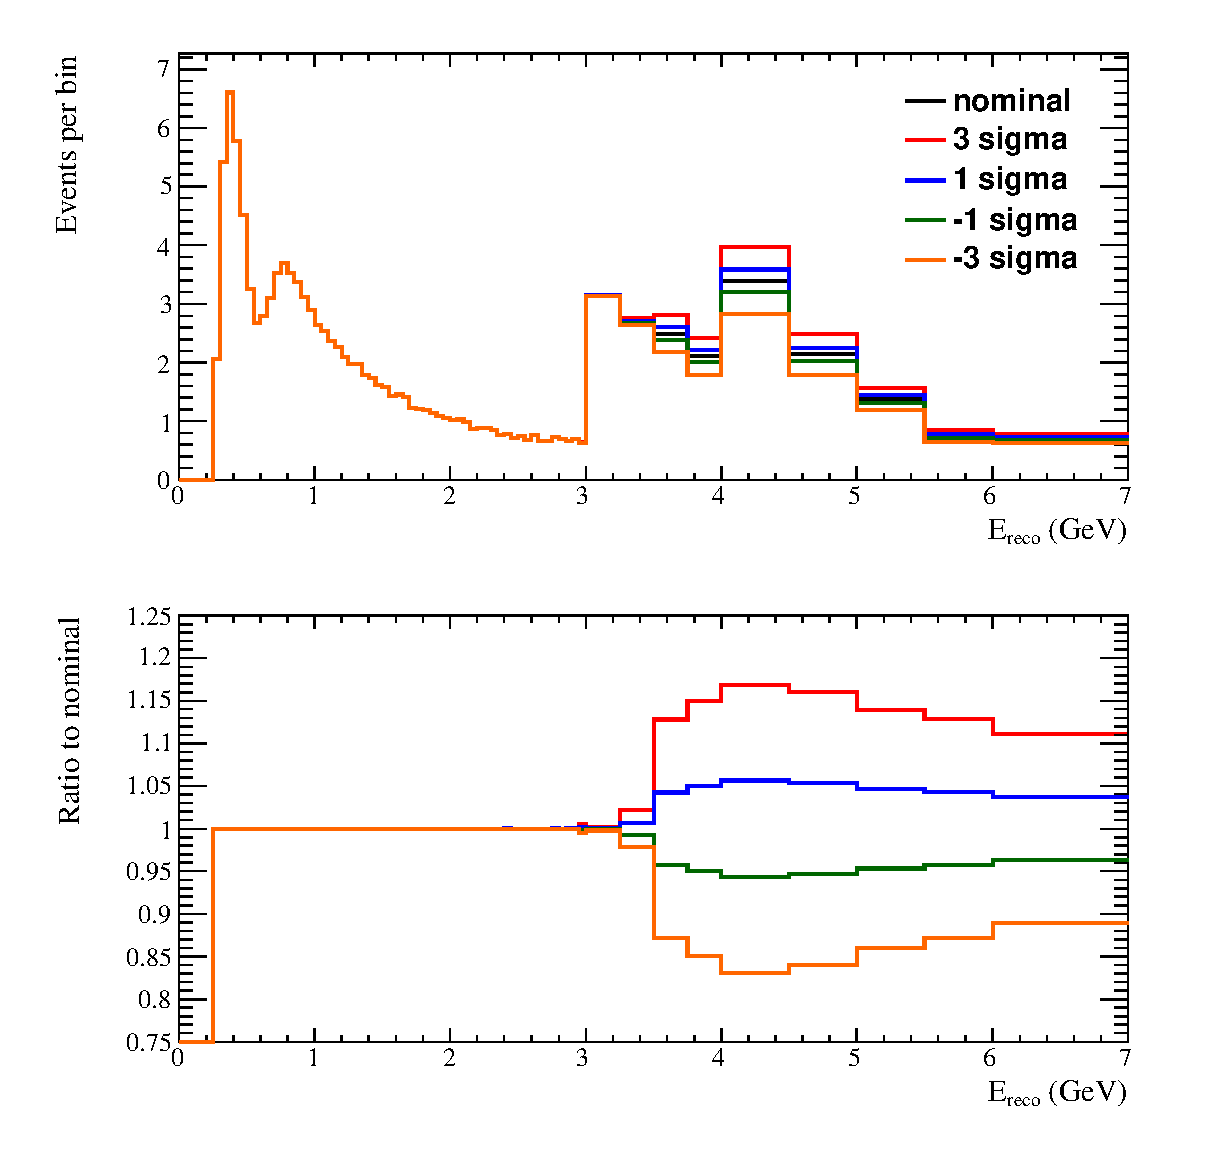
\includegraphics{../images/spectrum_tweaked/1sigma_oscillated/ereco_twk_f_banffccqee2}}
\caption
{ Effect of $f_{20; t, r}^{banff}$ for 3 flavour oscillations, using oscillation parameters:  $\sin^2\theta_{12} = $0.306; $\sin^2\theta_{13} = $0.0251; $\sin^2\theta_{23} = $0.5; $\delta_{CP} = $        0; $\Delta m^2_{21} = $    7.5e-05 eV$^2$/c$^4$; $|\Delta m^2_{32}| = $    0.0024 eV$^2$/c$^4$. }
\label{fig:osc_ereco_twk_f_banffccqee2}
\end{center}
\end{figure}
\clearpage

\begin{figure}
\begin{center}
\resizebox{14cm}{!}{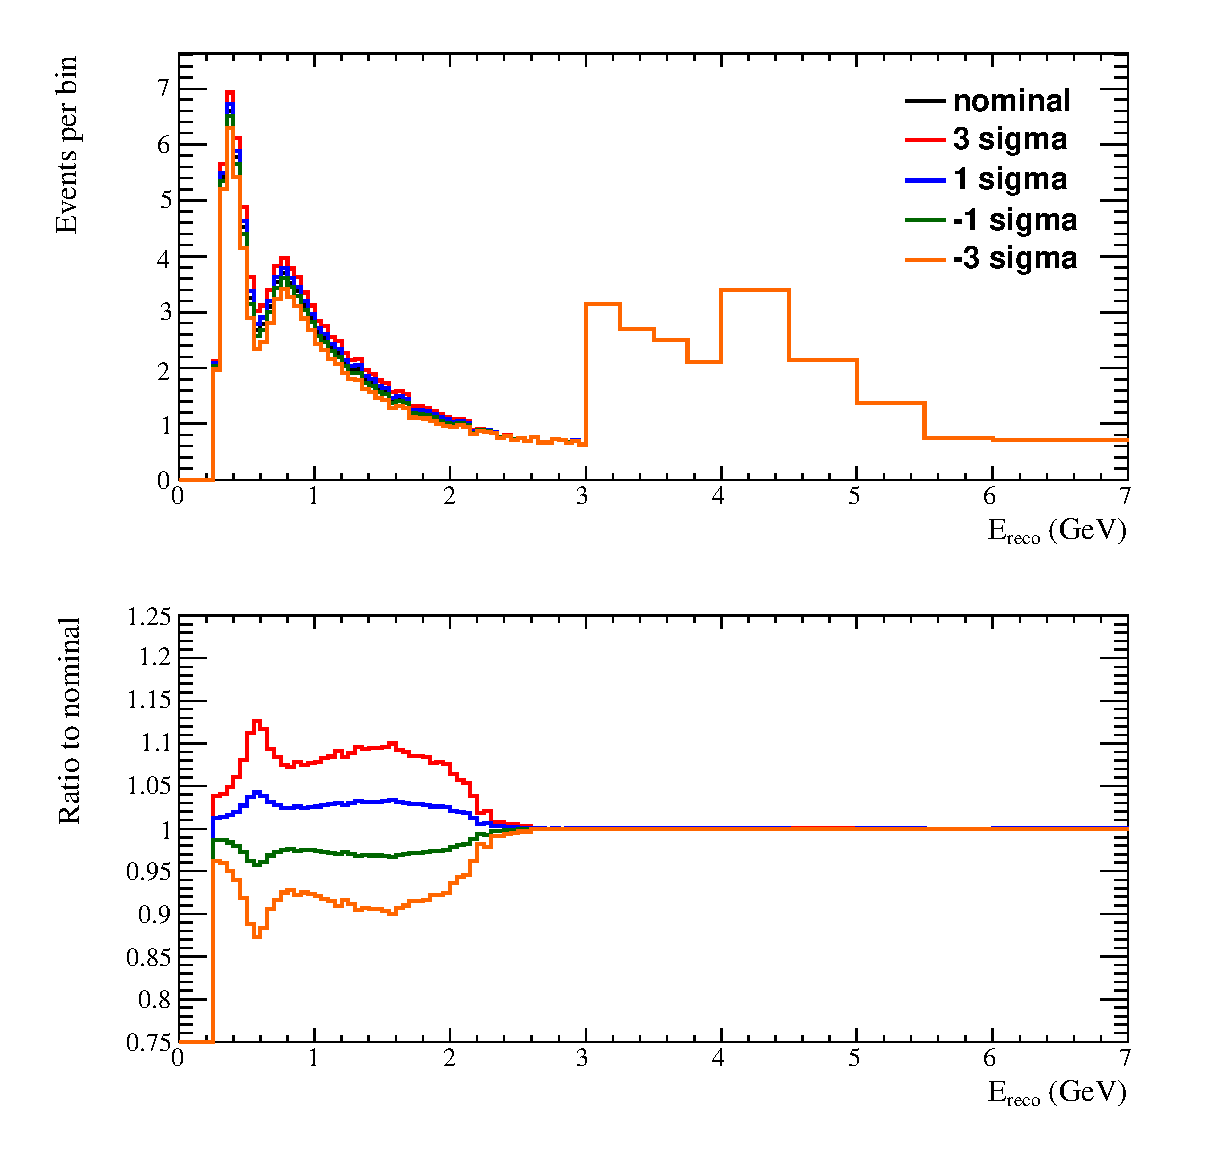
\includegraphics{../images/spectrum_tweaked/1sigma_oscillated/ereco_twk_f_banffcc1pie0}}
\caption
{ Effect of $f_{21; t, r}^{banff}$ for 3 flavour oscillations, using oscillation parameters:  $\sin^2\theta_{12} = $0.306; $\sin^2\theta_{13} = $0.0251; $\sin^2\theta_{23} = $0.5; $\delta_{CP} = $        0; $\Delta m^2_{21} = $    7.5e-05 eV$^2$/c$^4$; $|\Delta m^2_{32}| = $    0.0024 eV$^2$/c$^4$. }
\label{fig:osc_ereco_twk_f_banffcc1pie0}
\end{center}
\end{figure}
\clearpage

\begin{figure}
\begin{center}
\resizebox{14cm}{!}{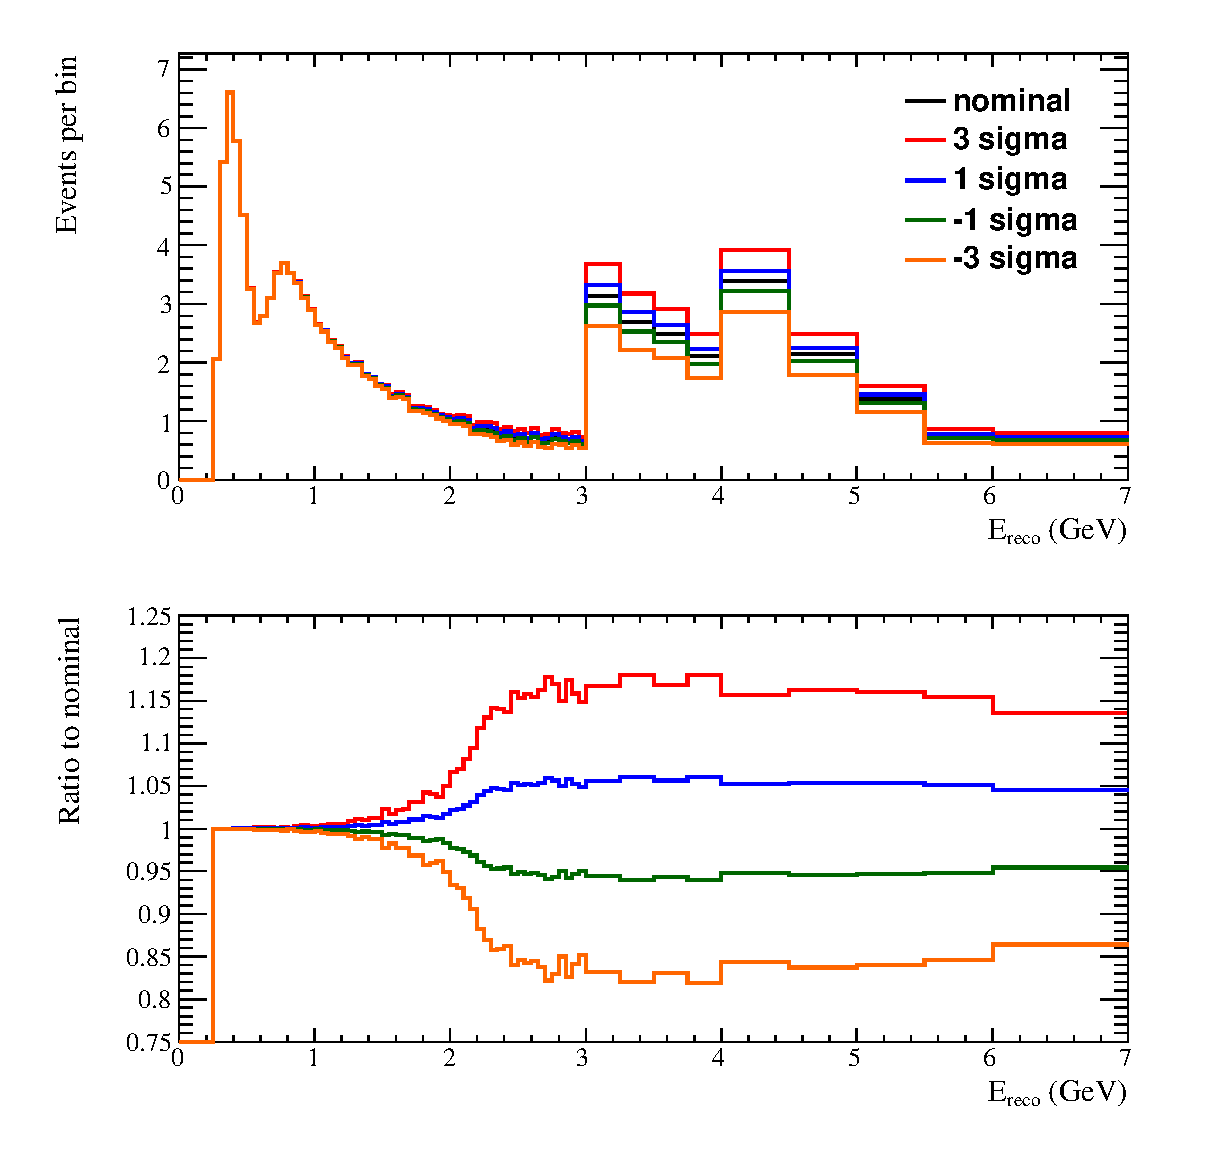
\includegraphics{../images/spectrum_tweaked/1sigma_oscillated/ereco_twk_f_banffcc1pie1}}
\caption
{ Effect of $f_{22; t, r}^{banff}$ for 3 flavour oscillations, using oscillation parameters:  $\sin^2\theta_{12} = $0.306; $\sin^2\theta_{13} = $0.0251; $\sin^2\theta_{23} = $0.5; $\delta_{CP} = $        0; $\Delta m^2_{21} = $    7.5e-05 eV$^2$/c$^4$; $|\Delta m^2_{32}| = $    0.0024 eV$^2$/c$^4$. }
\label{fig:osc_ereco_twk_f_banffcc1pie1}
\end{center}
\end{figure}
\clearpage

\begin{figure}
\begin{center}
\resizebox{14cm}{!}{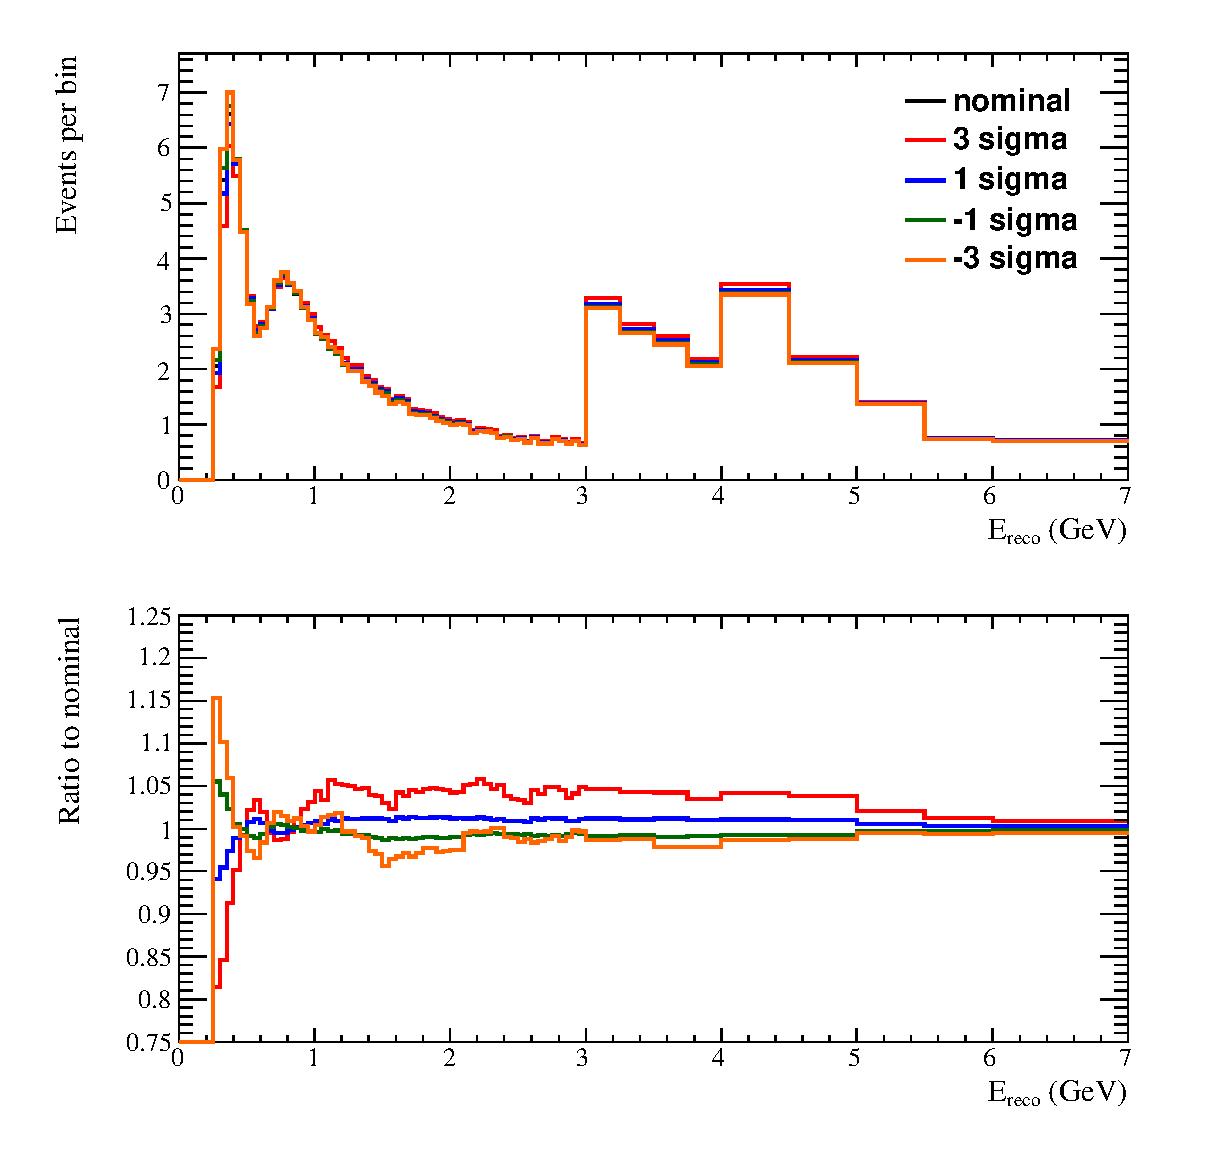
\includegraphics{../images/spectrum_tweaked/1sigma_oscillated/ereco_twk_f_pfermi}}
\caption
{ Effect of $f_{pF; t, r}$ for 3 flavour oscillations, using oscillation parameters:  $\sin^2\theta_{12} = $0.306; $\sin^2\theta_{13} = $0.0251; $\sin^2\theta_{23} = $0.5; $\delta_{CP} = $        0; $\Delta m^2_{21} = $    7.5e-05 eV$^2$/c$^4$; $|\Delta m^2_{32}| = $    0.0024 eV$^2$/c$^4$. }
\label{fig:osc_ereco_twk_f_pfermi}
\end{center}
\end{figure}
\clearpage

\begin{figure}
\begin{center}
\resizebox{14cm}{!}{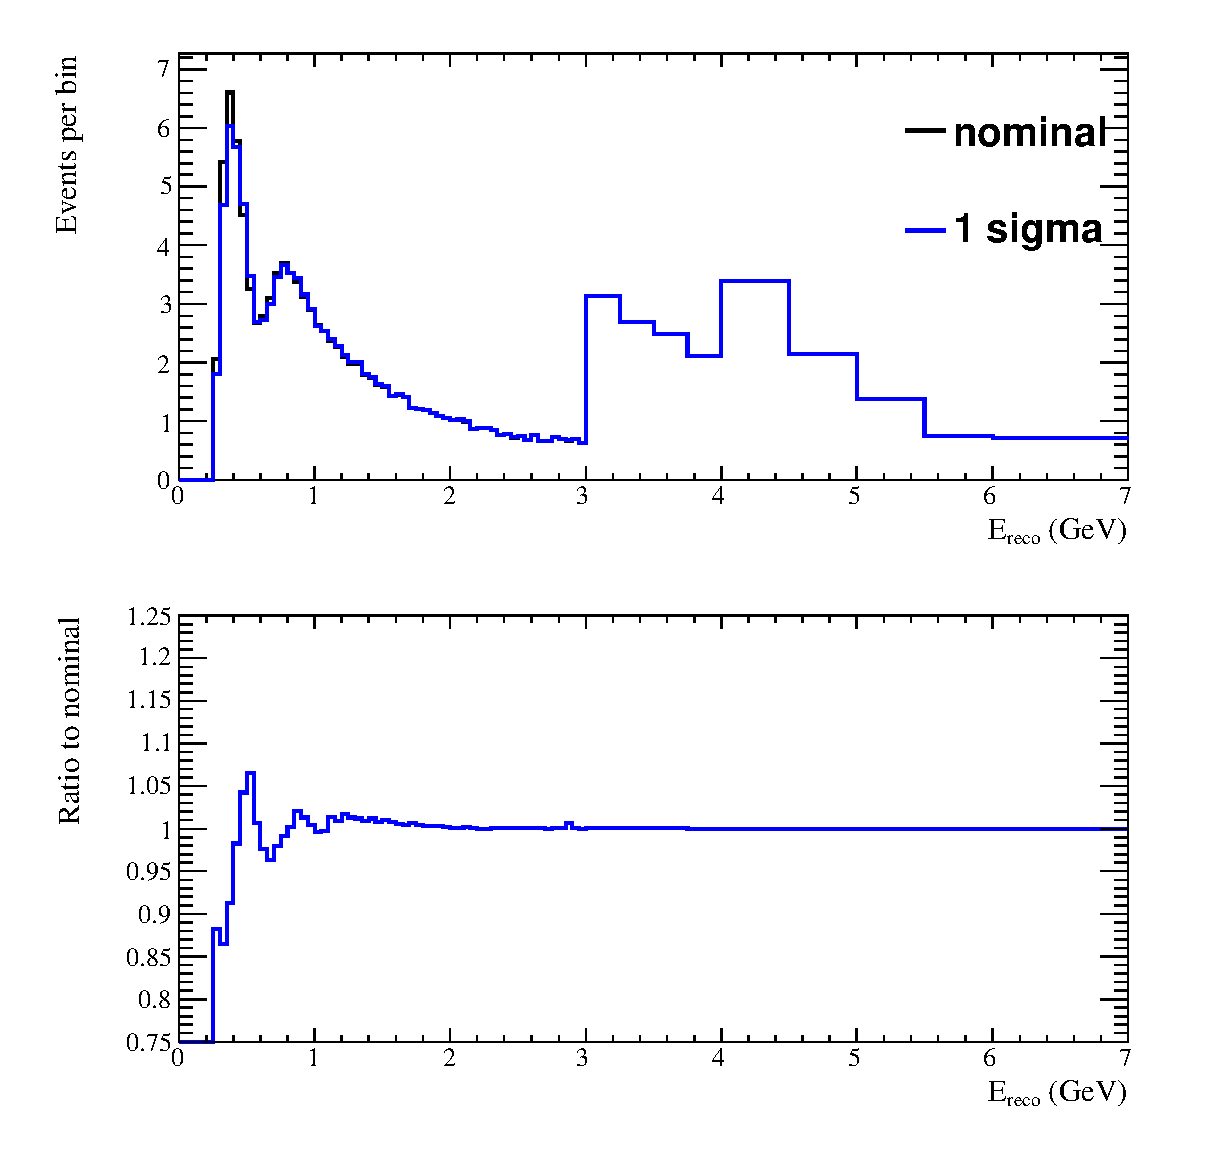
\includegraphics{../images/spectrum_tweaked/1sigma_oscillated/ereco_twk_f_specfunc}}
\caption
{ Effect of $f_{SF; t, r}$ for 3 flavour oscillations, using oscillation parameters:  $\sin^2\theta_{12} = $0.306; $\sin^2\theta_{13} = $0.0251; $\sin^2\theta_{23} = $0.5; $\delta_{CP} = $        0; $\Delta m^2_{21} = $    7.5e-05 eV$^2$/c$^4$; $|\Delta m^2_{32}| = $    0.0024 eV$^2$/c$^4$. }
\label{fig:osc_ereco_twk_f_specfunc}
\end{center}
\end{figure}
\clearpage

\begin{figure}
\begin{center}
\resizebox{14cm}{!}{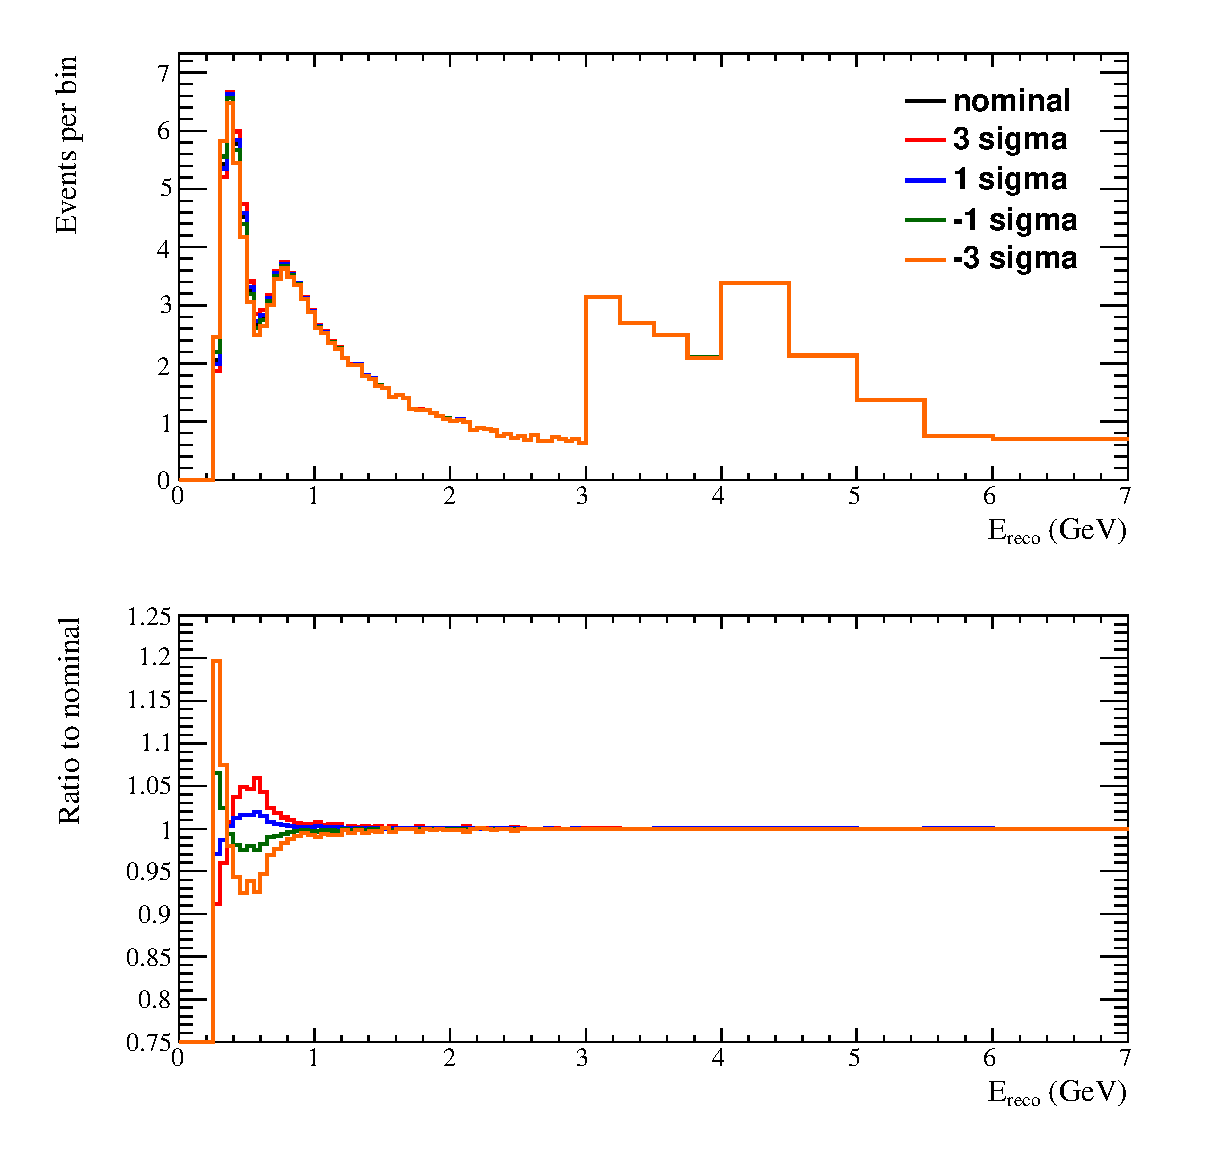
\includegraphics{../images/spectrum_tweaked/1sigma_oscillated/ereco_twk_f_wshape}}
\caption
{ Effect of $f_{Wshape; t, r}$ for 3 flavour oscillations, using oscillation parameters:  $\sin^2\theta_{12} = $0.306; $\sin^2\theta_{13} = $0.0251; $\sin^2\theta_{23} = $0.5; $\delta_{CP} = $        0; $\Delta m^2_{21} = $    7.5e-05 eV$^2$/c$^4$; $|\Delta m^2_{32}| = $    0.0024 eV$^2$/c$^4$. }
\label{fig:osc_ereco_twk_f_wshape}
\end{center}
\end{figure}
\clearpage

\begin{figure}
\begin{center}
\resizebox{14cm}{!}{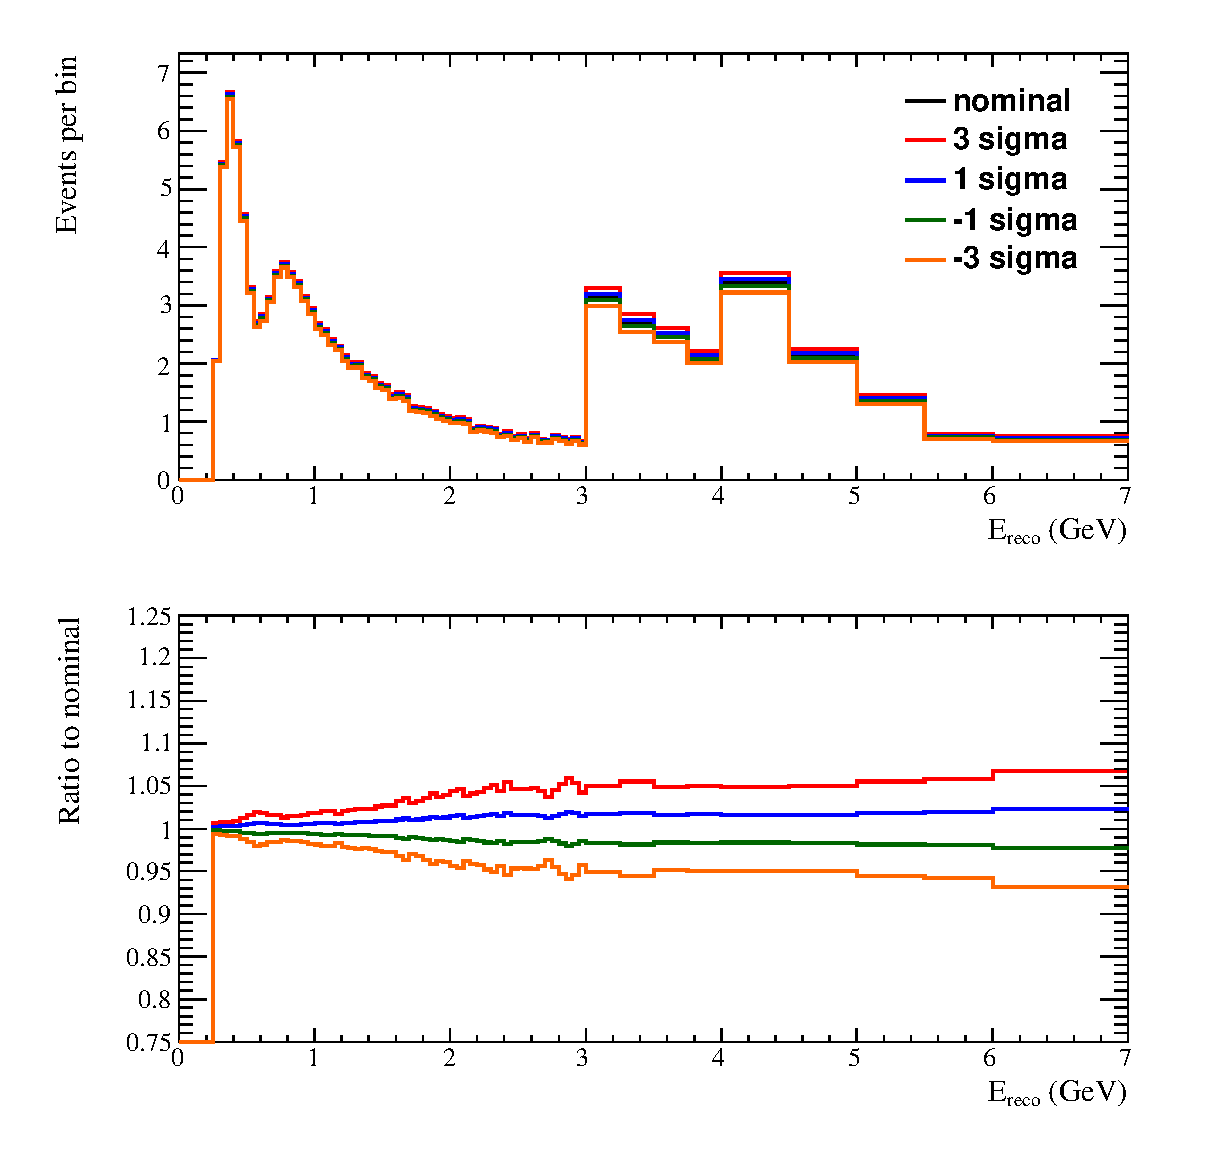
\includegraphics{../images/spectrum_tweaked/1sigma_oscillated/ereco_twk_f_shapeCCoth}}
\caption
{ Effect of $f_{CCothShape; t, r}$ for 3 flavour oscillations, using oscillation parameters:  $\sin^2\theta_{12} = $0.306; $\sin^2\theta_{13} = $0.0251; $\sin^2\theta_{23} = $0.5; $\delta_{CP} = $        0; $\Delta m^2_{21} = $    7.5e-05 eV$^2$/c$^4$; $|\Delta m^2_{32}| = $    0.0024 eV$^2$/c$^4$. }
\label{fig:osc_ereco_twk_f_shapeCCoth}
\end{center}
\end{figure}
\clearpage

\begin{figure}
\begin{center}
\resizebox{14cm}{!}{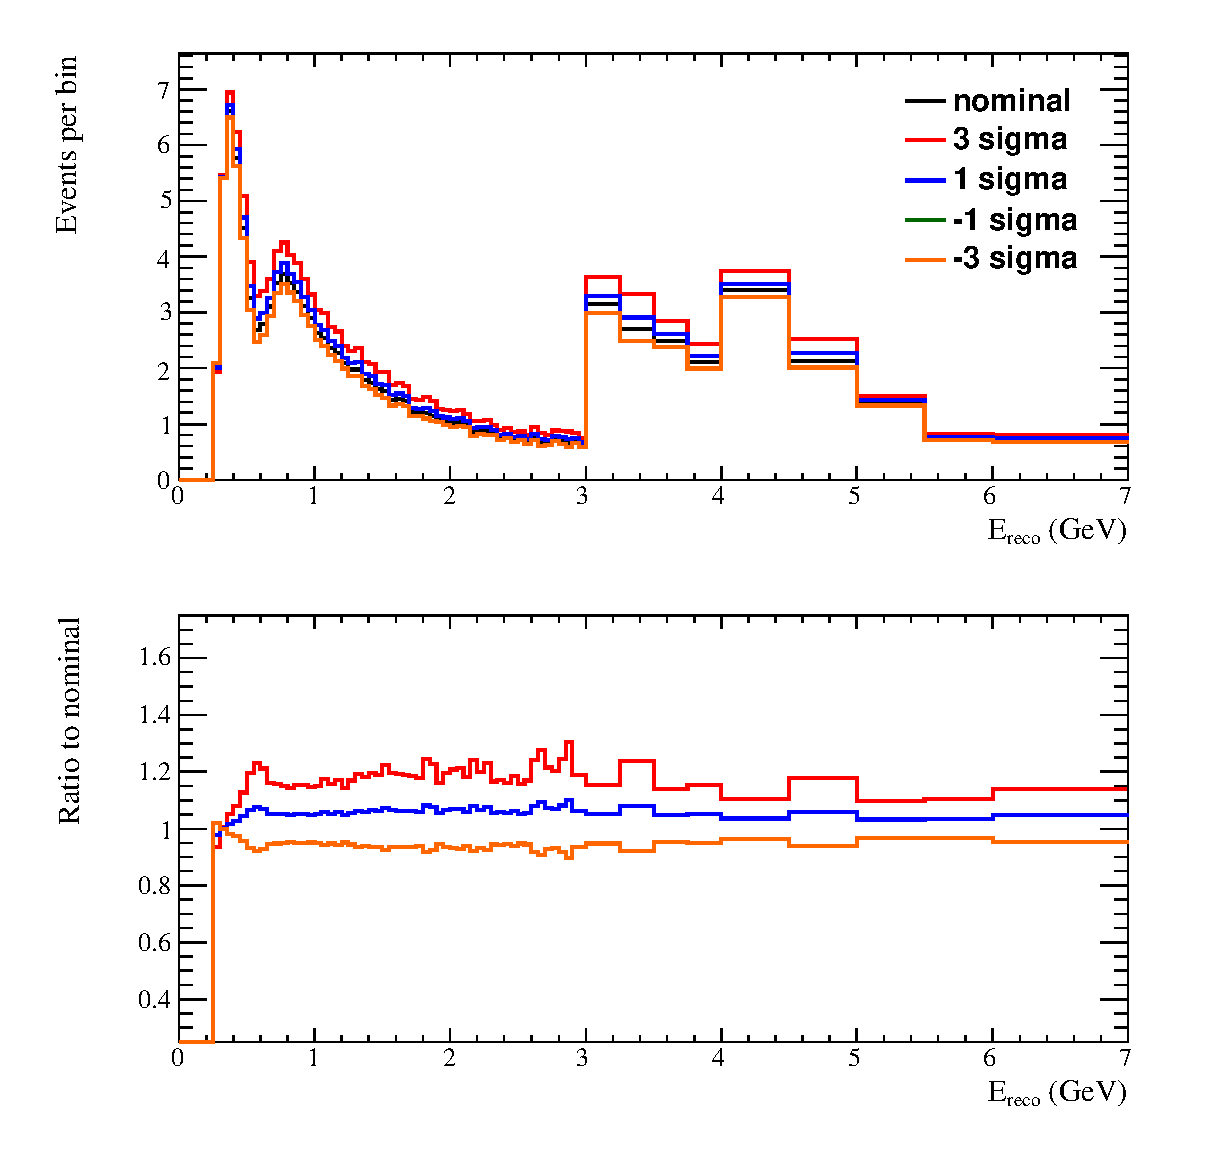
\includegraphics{../images/spectrum_tweaked/1sigma_oscillated/ereco_twk_f_pilessdelta}}
\caption
{ Effect of $f_{\pi-less\Delta; t, r}$ for 3 flavour oscillations, using oscillation parameters:  $\sin^2\theta_{12} = $0.306; $\sin^2\theta_{13} = $0.0251; $\sin^2\theta_{23} = $0.5; $\delta_{CP} = $        0; $\Delta m^2_{21} = $    7.5e-05 eV$^2$/c$^4$; $|\Delta m^2_{32}| = $    0.0024 eV$^2$/c$^4$. }
\label{fig:osc_ereco_twk_f_pilessdelta}
\end{center}
\end{figure}
\clearpage

\begin{figure}
\begin{center}
\resizebox{14cm}{!}{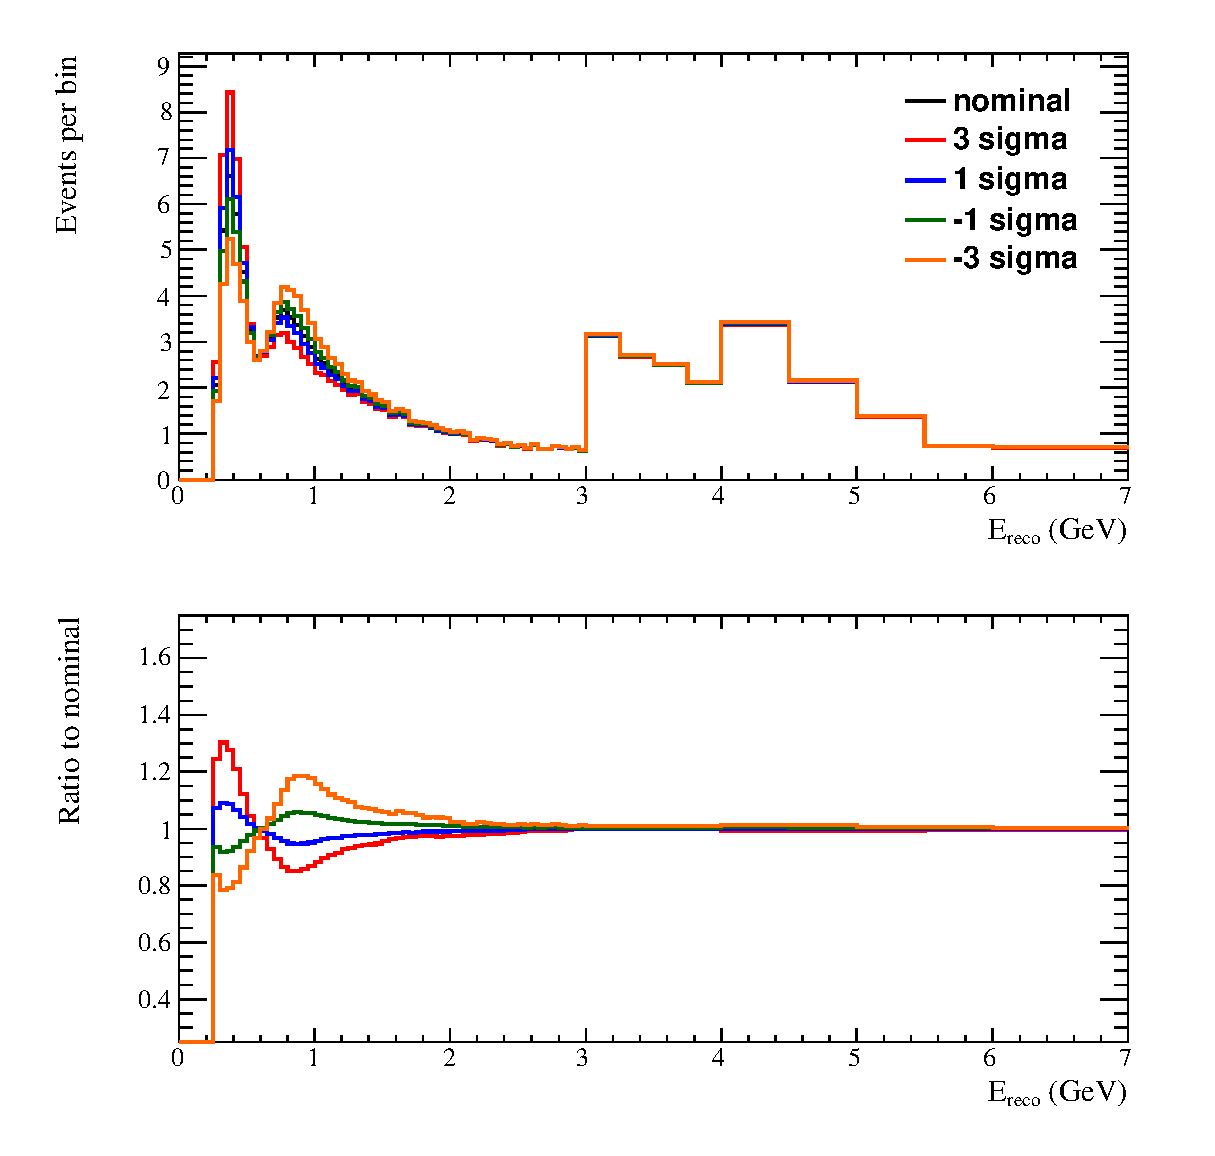
\includegraphics{../images/spectrum_tweaked/1sigma_oscillated/ereco_twk_f_bindE}}
\caption
{ Effect of $f_{bindE; t, r}$ for 3 flavour oscillations, using oscillation parameters:  $\sin^2\theta_{12} = $0.306; $\sin^2\theta_{13} = $0.0251; $\sin^2\theta_{23} = $0.5; $\delta_{CP} = $        0; $\Delta m^2_{21} = $    7.5e-05 eV$^2$/c$^4$; $|\Delta m^2_{32}| = $    0.0024 eV$^2$/c$^4$. }
\label{fig:osc_ereco_twk_f_bindE}
\end{center}
\end{figure}
\clearpage

\begin{figure}
\begin{center}
\resizebox{14cm}{!}{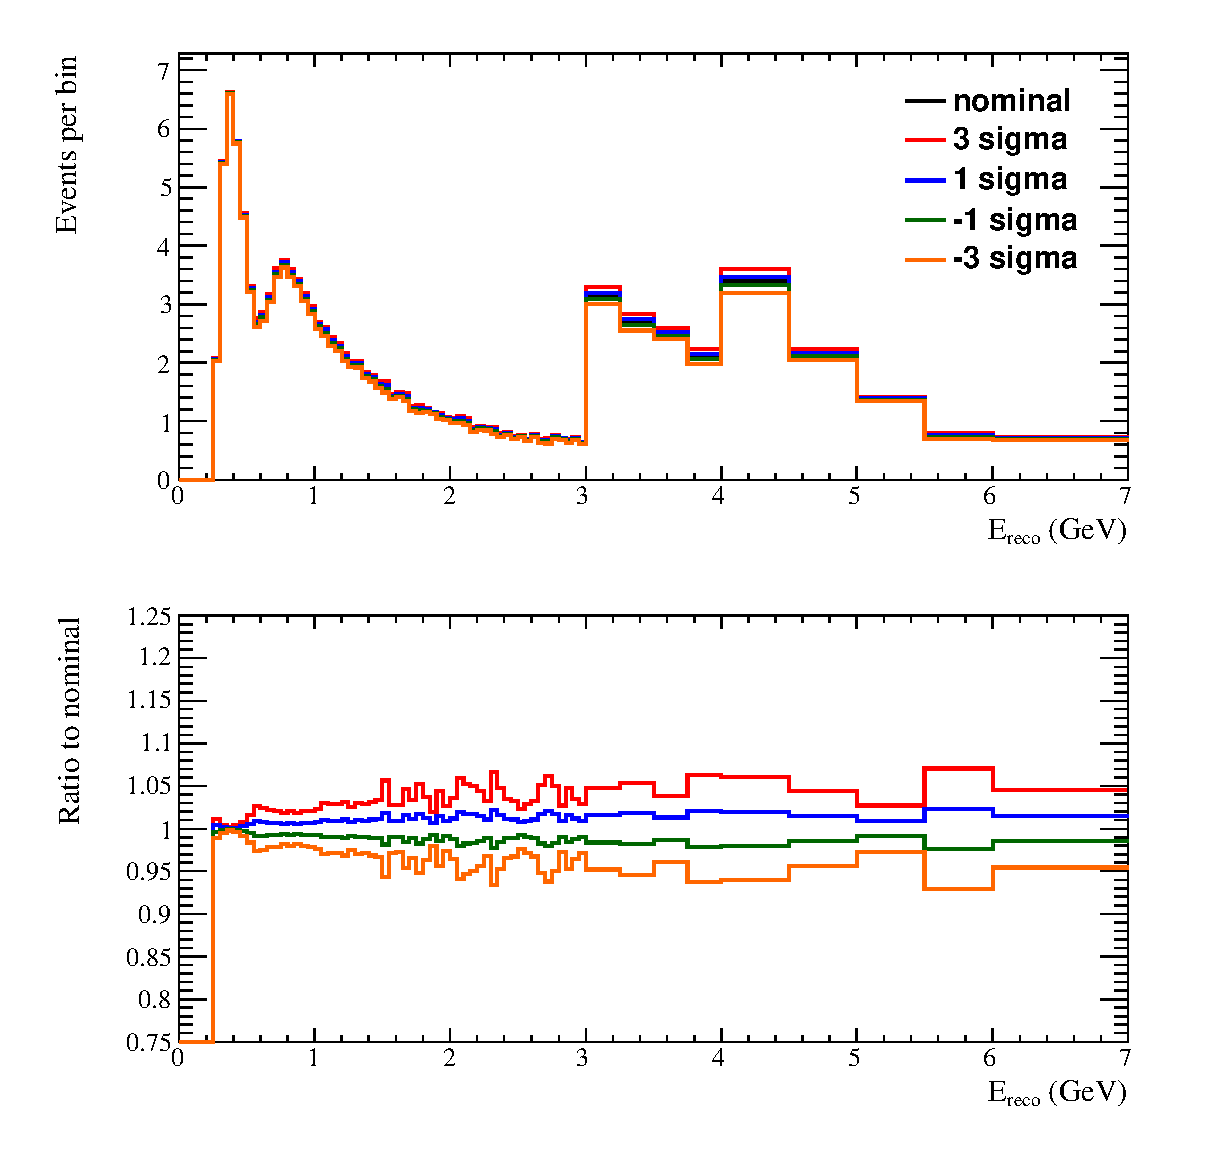
\includegraphics{../images/spectrum_tweaked/1sigma_oscillated/ereco_twk_f_norm_cccoh}}
\caption
{ Effect of $f_{CCcoh; t}$ for 3 flavour oscillations, using oscillation parameters:  $\sin^2\theta_{12} = $0.306; $\sin^2\theta_{13} = $0.0251; $\sin^2\theta_{23} = $0.5; $\delta_{CP} = $        0; $\Delta m^2_{21} = $    7.5e-05 eV$^2$/c$^4$; $|\Delta m^2_{32}| = $    0.0024 eV$^2$/c$^4$. }
\label{fig:osc_ereco_twk_f_norm_cccoh}
\end{center}
\end{figure}
\clearpage

\begin{figure}
\begin{center}
\resizebox{14cm}{!}{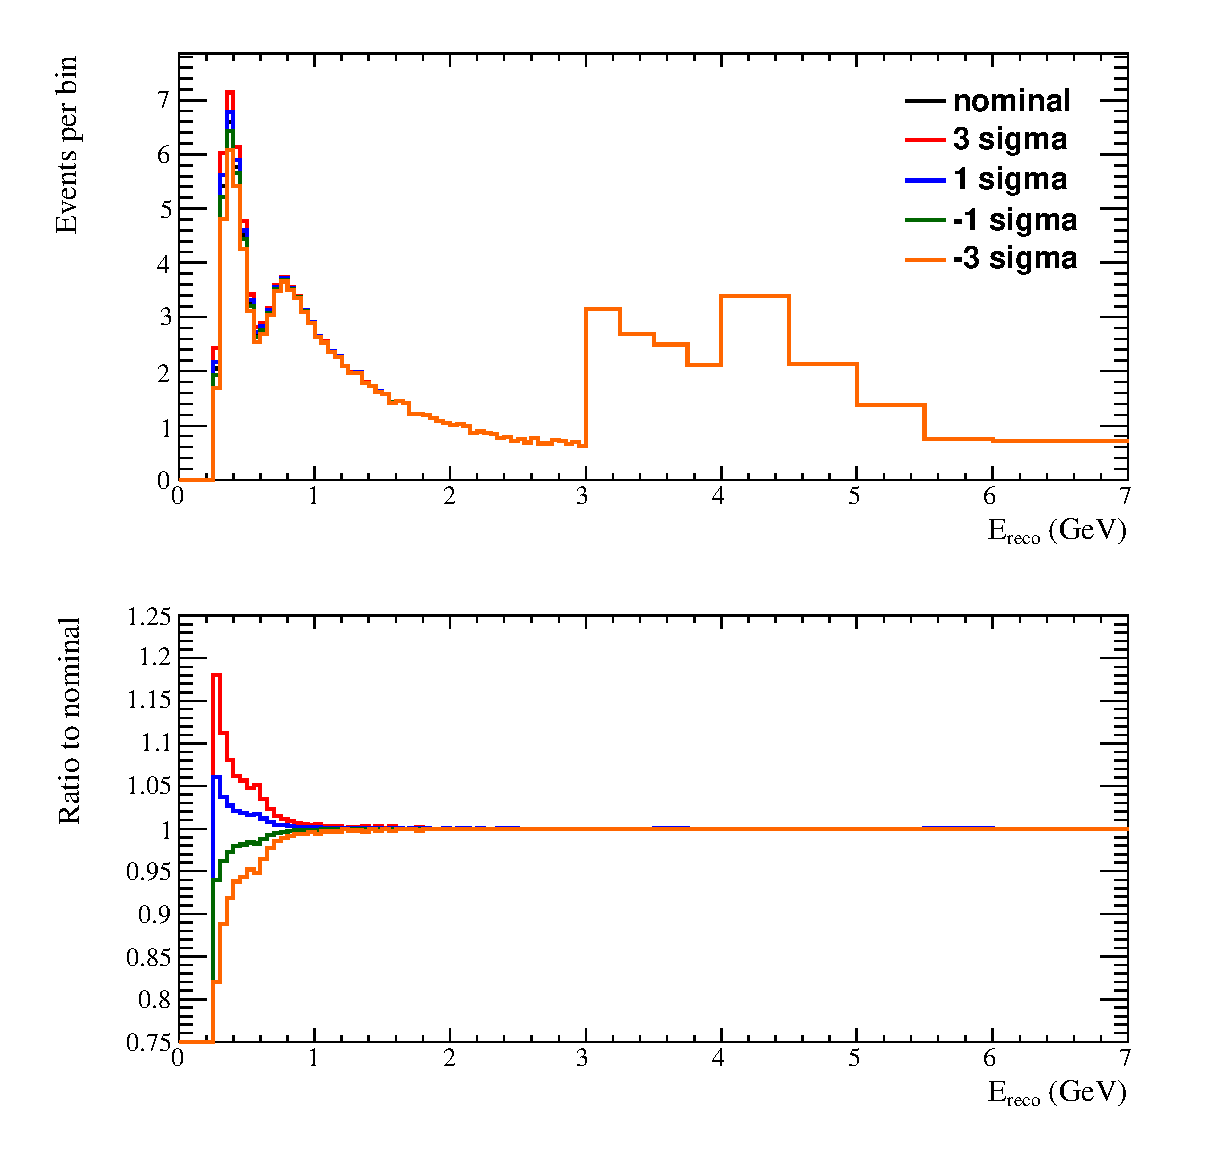
\includegraphics{../images/spectrum_tweaked/1sigma_oscillated/ereco_twk_f_norm_nc1piC}}
\caption
{ Effect of $f_{NC1\pi^\pm; t}$ for 3 flavour oscillations, using oscillation parameters:  $\sin^2\theta_{12} = $0.306; $\sin^2\theta_{13} = $0.0251; $\sin^2\theta_{23} = $0.5; $\delta_{CP} = $        0; $\Delta m^2_{21} = $    7.5e-05 eV$^2$/c$^4$; $|\Delta m^2_{32}| = $    0.0024 eV$^2$/c$^4$. }
\label{fig:osc_ereco_twk_f_norm_nc1piC}
\end{center}
\end{figure}
\clearpage

\begin{figure}
\begin{center}
\resizebox{14cm}{!}{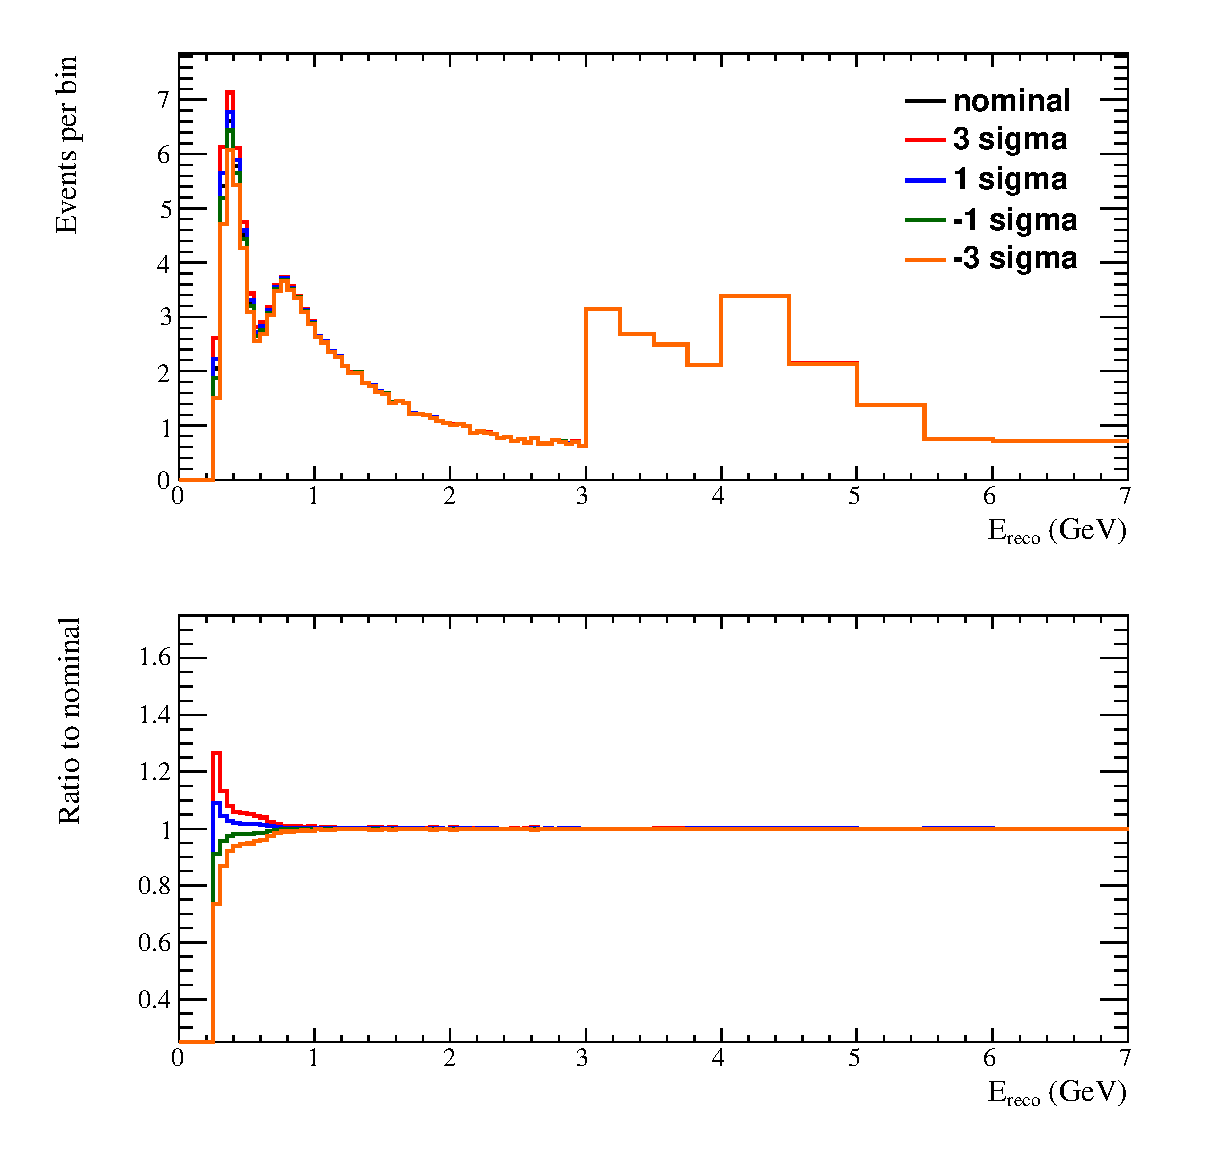
\includegraphics{../images/spectrum_tweaked/1sigma_oscillated/ereco_twk_f_norm_ncoth}}
\caption
{ Effect of $f_{NCoth; t}$ for 3 flavour oscillations, using oscillation parameters:  $\sin^2\theta_{12} = $0.306; $\sin^2\theta_{13} = $0.0251; $\sin^2\theta_{23} = $0.5; $\delta_{CP} = $        0; $\Delta m^2_{21} = $    7.5e-05 eV$^2$/c$^4$; $|\Delta m^2_{32}| = $    0.0024 eV$^2$/c$^4$. }
\label{fig:osc_ereco_twk_f_norm_ncoth}
\end{center}
\end{figure}
\clearpage

\begin{figure}
\begin{center}
\resizebox{14cm}{!}{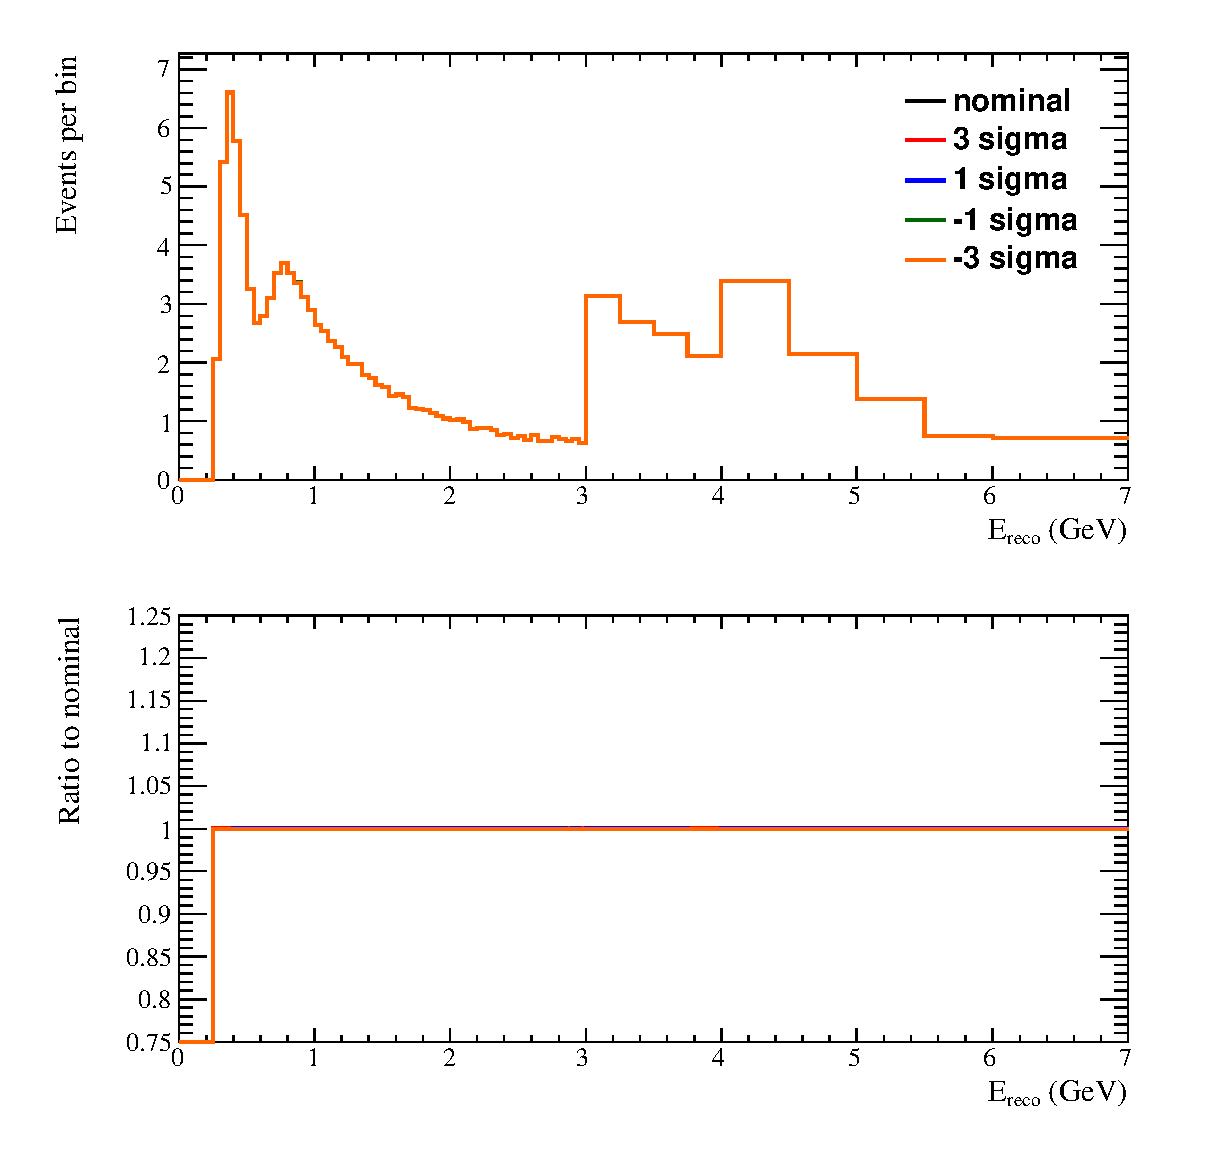
\includegraphics{../images/spectrum_tweaked/1sigma_oscillated/ereco_twk_f_norm_nuetonumu}}
\caption
{ Effect of $f_{CC\nu_e; t}$ for 3 flavour oscillations, using oscillation parameters:  $\sin^2\theta_{12} = $0.306; $\sin^2\theta_{13} = $0.0251; $\sin^2\theta_{23} = $0.5; $\delta_{CP} = $        0; $\Delta m^2_{21} = $    7.5e-05 eV$^2$/c$^4$; $|\Delta m^2_{32}| = $    0.0024 eV$^2$/c$^4$. }
\label{fig:osc_ereco_twk_f_norm_nuetonumu}
\end{center}
\end{figure}
\clearpage

\begin{figure}
\begin{center}
\resizebox{14cm}{!}{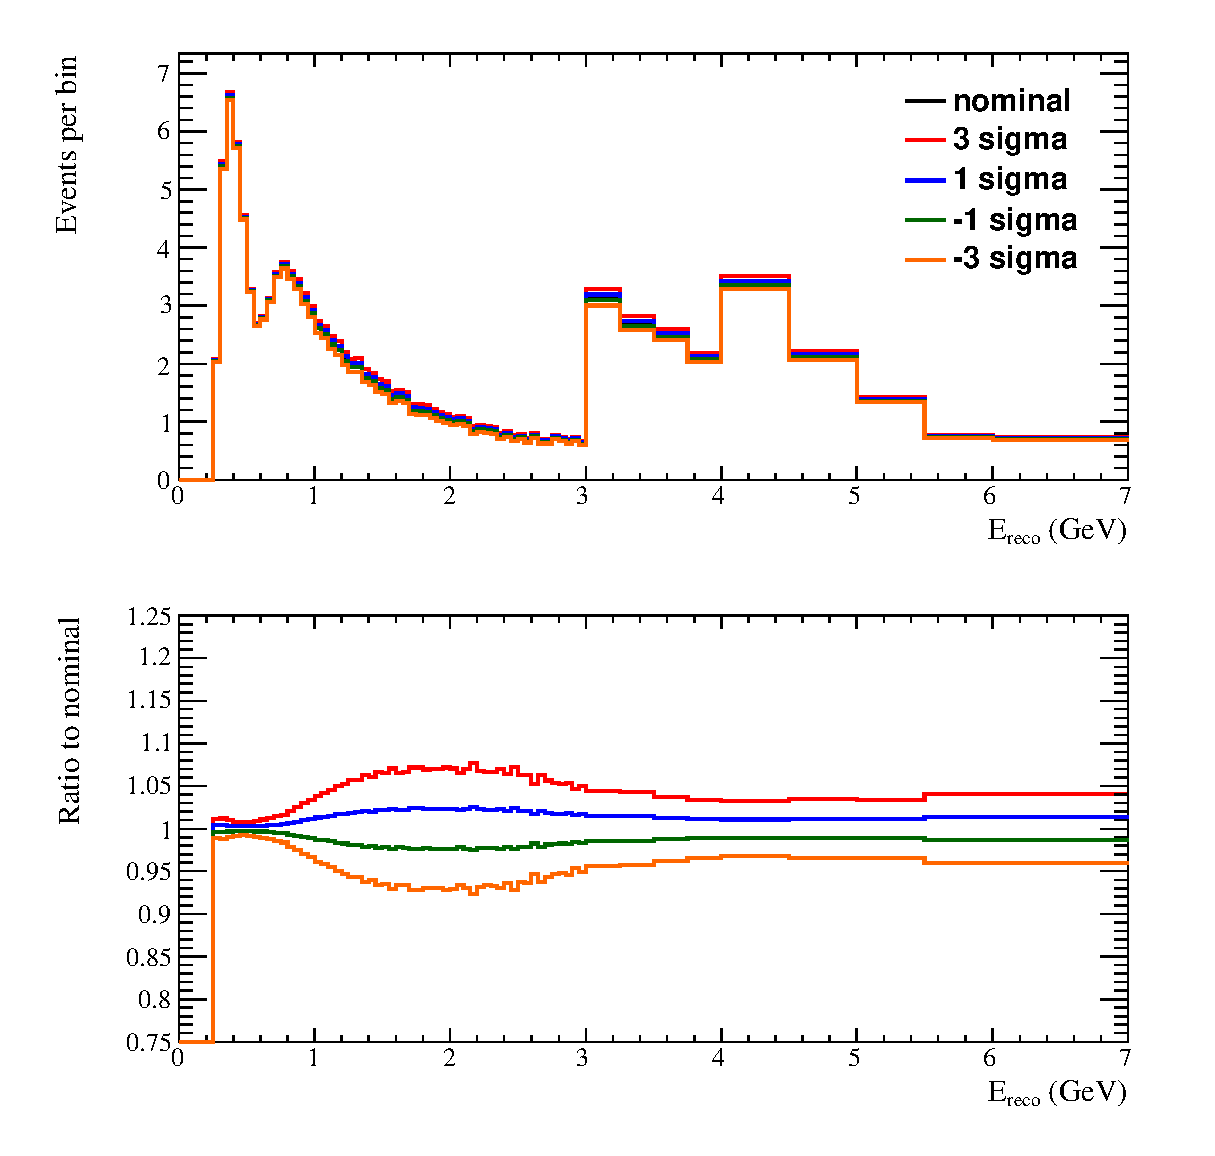
\includegraphics{../images/spectrum_tweaked/1sigma_oscillated/ereco_twk_f_norm_antinutonu}}
\caption
{ Effect of $f_{CC\bar{\nu}; t}$ for 3 flavour oscillations, using oscillation parameters:  $\sin^2\theta_{12} = $0.306; $\sin^2\theta_{13} = $0.0251; $\sin^2\theta_{23} = $0.5; $\delta_{CP} = $        0; $\Delta m^2_{21} = $    7.5e-05 eV$^2$/c$^4$; $|\Delta m^2_{32}| = $    0.0024 eV$^2$/c$^4$. }
\label{fig:osc_ereco_twk_f_norm_antinutonu}
\end{center}
\end{figure}
\clearpage

\begin{figure}
\begin{center}
\resizebox{14cm}{!}{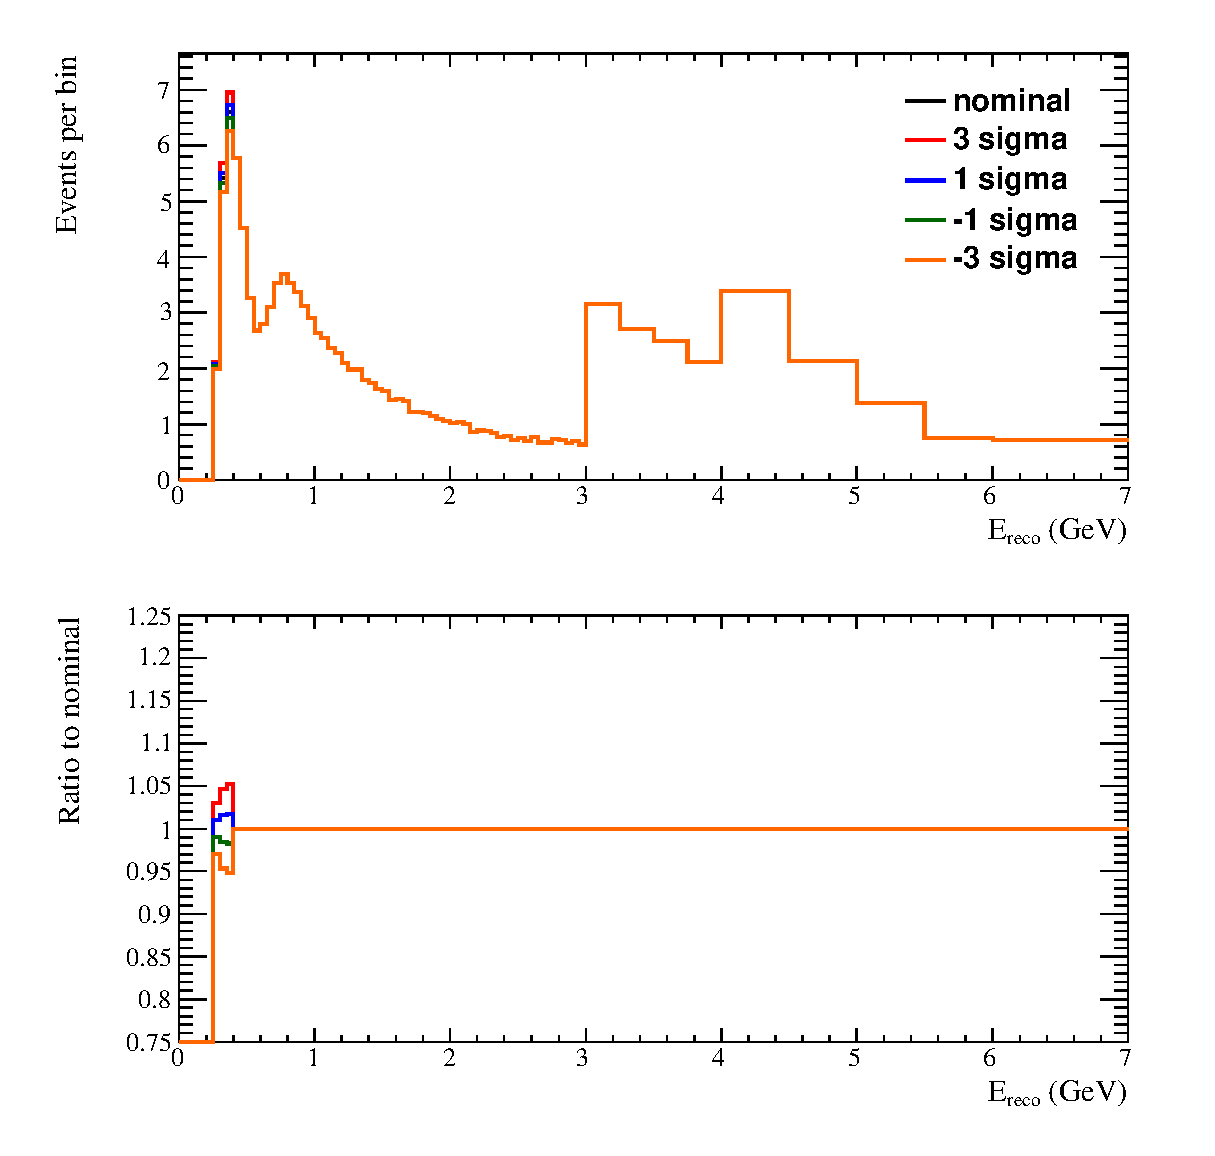
\includegraphics{../images/spectrum_tweaked/1sigma_oscillated/ereco_twk_f_skdetfsi000}}
\caption
{ Effect of $f_{0; r}^{SK+FSI}$ for 3 flavour oscillations, using oscillation parameters:  $\sin^2\theta_{12} = $0.306; $\sin^2\theta_{13} = $0.0251; $\sin^2\theta_{23} = $0.5; $\delta_{CP} = $        0; $\Delta m^2_{21} = $    7.5e-05 eV$^2$/c$^4$; $|\Delta m^2_{32}| = $    0.0024 eV$^2$/c$^4$. }
\label{fig:osc_ereco_twk_f_skdetfsi000}
\end{center}
\end{figure}
\clearpage

\begin{figure}
\begin{center}
\resizebox{14cm}{!}{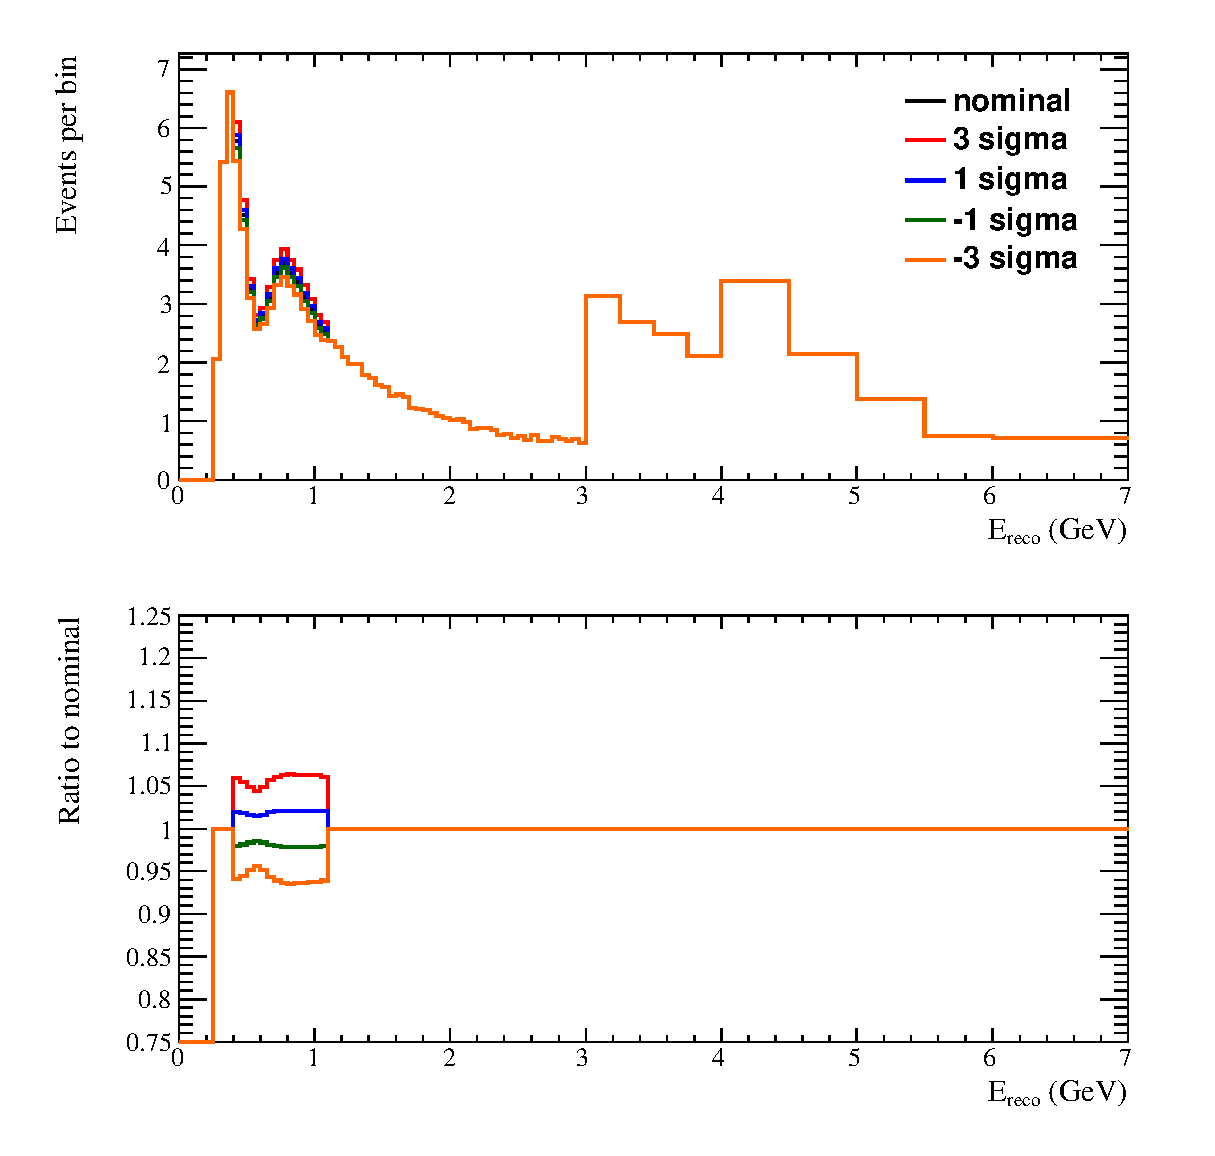
\includegraphics{../images/spectrum_tweaked/1sigma_oscillated/ereco_twk_f_skdetfsi001}}
\caption
{ Effect of $f_{1; r}^{SK+FSI}$ for 3 flavour oscillations, using oscillation parameters:  $\sin^2\theta_{12} = $0.306; $\sin^2\theta_{13} = $0.0251; $\sin^2\theta_{23} = $0.5; $\delta_{CP} = $        0; $\Delta m^2_{21} = $    7.5e-05 eV$^2$/c$^4$; $|\Delta m^2_{32}| = $    0.0024 eV$^2$/c$^4$. }
\label{fig:osc_ereco_twk_f_skdetfsi001}
\end{center}
\end{figure}
\clearpage

\begin{figure}
\begin{center}
\resizebox{14cm}{!}{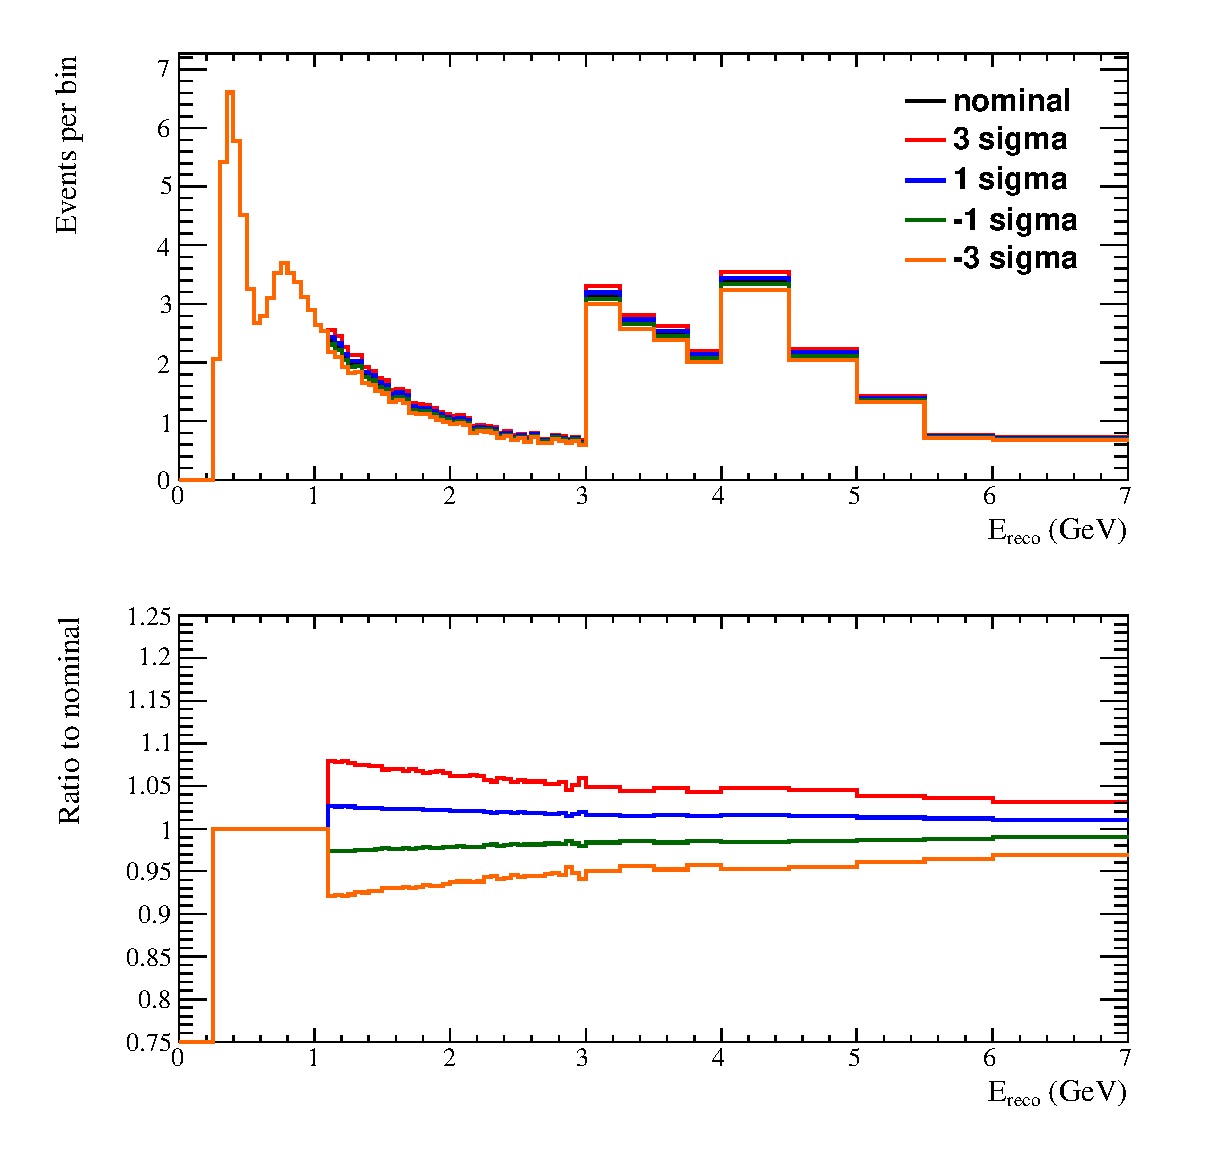
\includegraphics{../images/spectrum_tweaked/1sigma_oscillated/ereco_twk_f_skdetfsi002}}
\caption
{ Effect of $f_{2; r}^{SK+FSI}$ for 3 flavour oscillations, using oscillation parameters:  $\sin^2\theta_{12} = $0.306; $\sin^2\theta_{13} = $0.0251; $\sin^2\theta_{23} = $0.5; $\delta_{CP} = $        0; $\Delta m^2_{21} = $    7.5e-05 eV$^2$/c$^4$; $|\Delta m^2_{32}| = $    0.0024 eV$^2$/c$^4$. }
\label{fig:osc_ereco_twk_f_skdetfsi002}
\end{center}
\end{figure}
\clearpage

\begin{figure}
\begin{center}
\resizebox{14cm}{!}{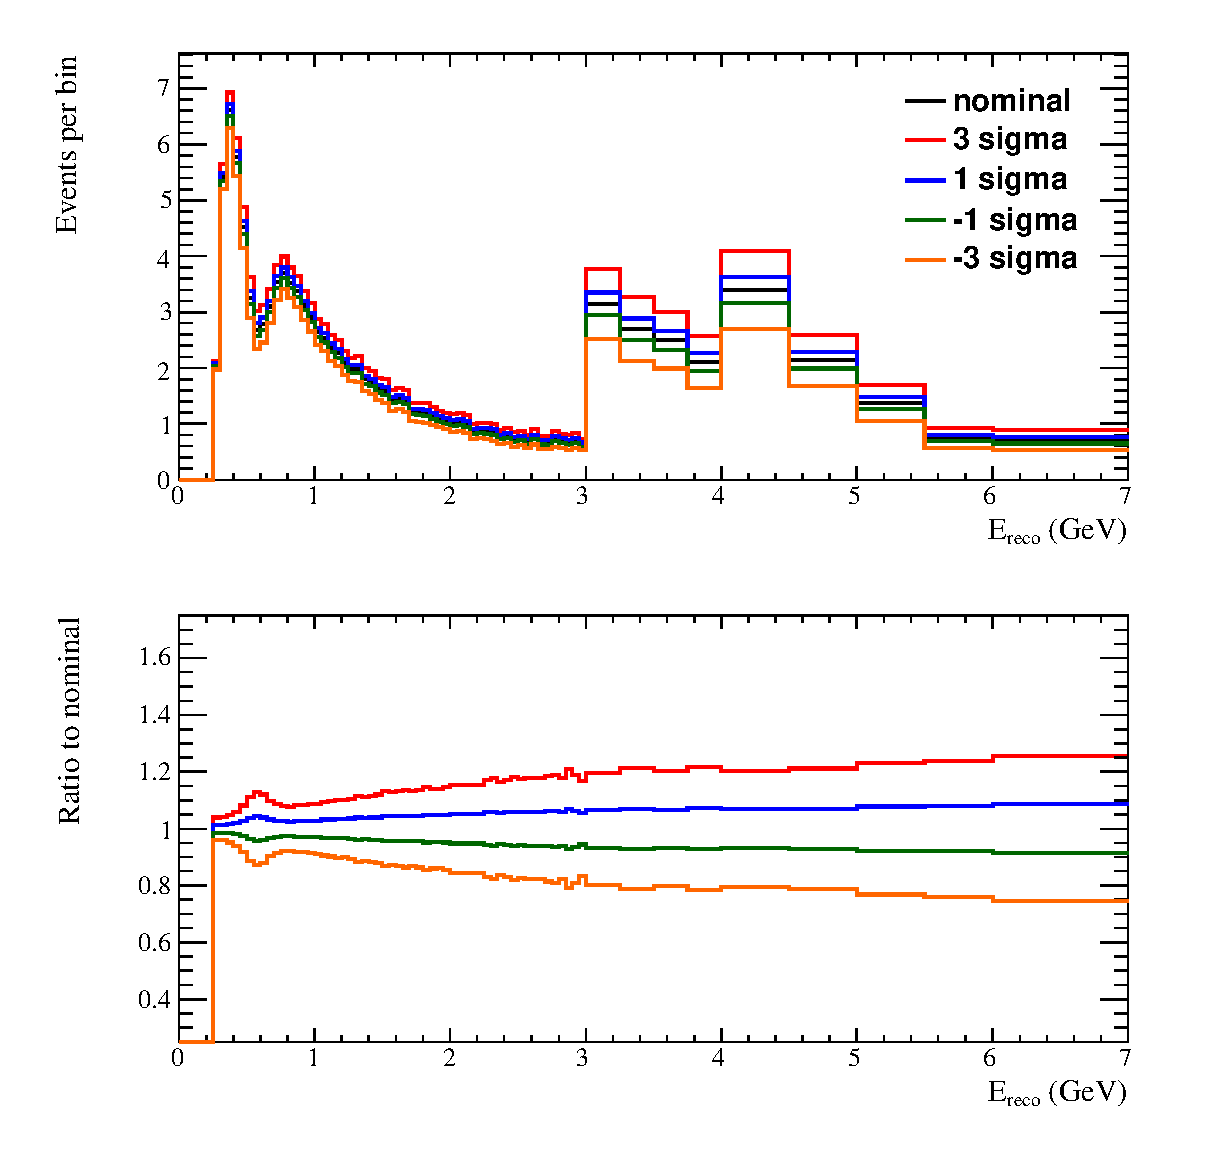
\includegraphics{../images/spectrum_tweaked/1sigma_oscillated/ereco_twk_f_skdetfsi003}}
\caption
{ Effect of $f_{3; r}^{SK+FSI}$ for 3 flavour oscillations, using oscillation parameters:  $\sin^2\theta_{12} = $0.306; $\sin^2\theta_{13} = $0.0251; $\sin^2\theta_{23} = $0.5; $\delta_{CP} = $        0; $\Delta m^2_{21} = $    7.5e-05 eV$^2$/c$^4$; $|\Delta m^2_{32}| = $    0.0024 eV$^2$/c$^4$. }
\label{fig:osc_ereco_twk_f_skdetfsi003}
\end{center}
\end{figure}
\clearpage

\begin{figure}
\begin{center}
\resizebox{14cm}{!}{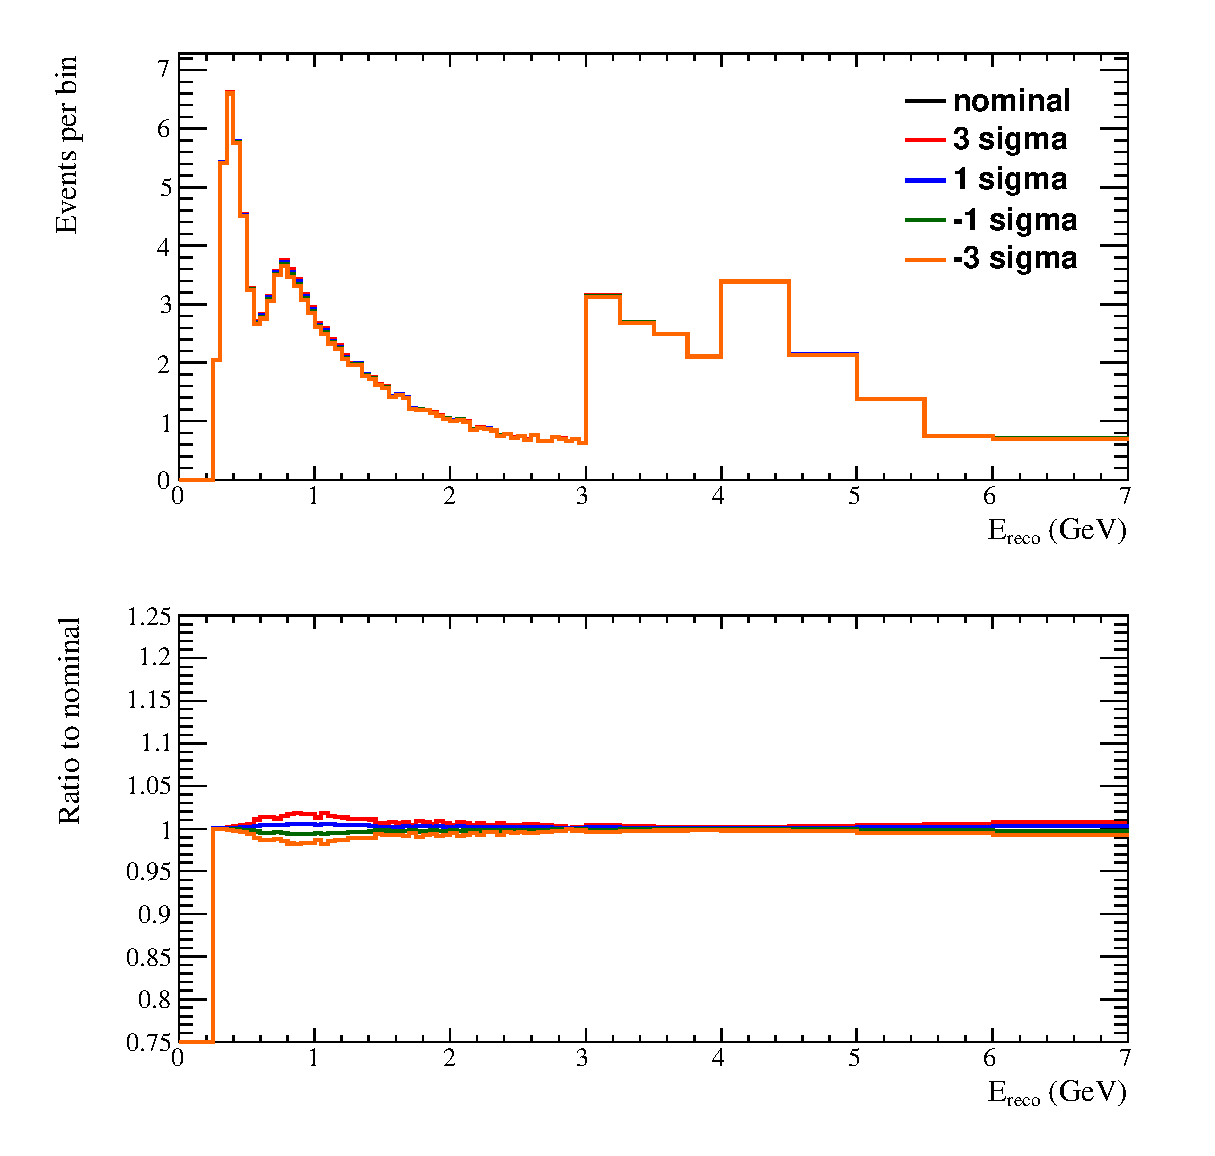
\includegraphics{../images/spectrum_tweaked/1sigma_oscillated/ereco_twk_f_skdetfsi004}}
\caption
{ Effect of $f_{4; r}^{SK+FSI}$ for 3 flavour oscillations, using oscillation parameters:  $\sin^2\theta_{12} = $0.306; $\sin^2\theta_{13} = $0.0251; $\sin^2\theta_{23} = $0.5; $\delta_{CP} = $        0; $\Delta m^2_{21} = $    7.5e-05 eV$^2$/c$^4$; $|\Delta m^2_{32}| = $    0.0024 eV$^2$/c$^4$. }
\label{fig:osc_ereco_twk_f_skdetfsi004}
\end{center}
\end{figure}
\clearpage

\begin{figure}
\begin{center}
\resizebox{14cm}{!}{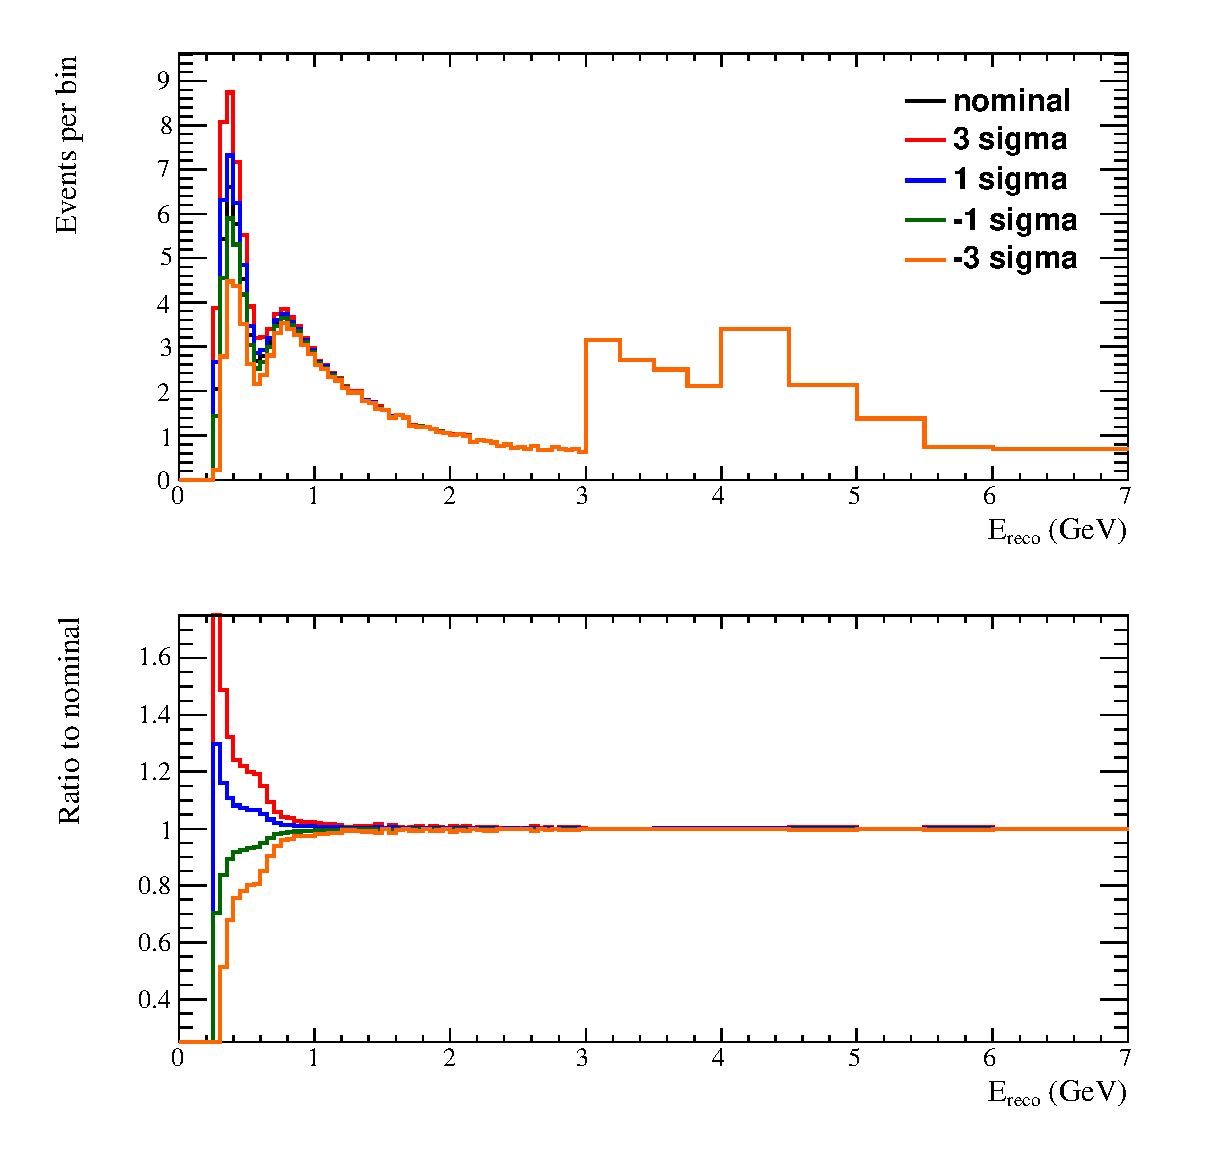
\includegraphics{../images/spectrum_tweaked/1sigma_oscillated/ereco_twk_f_skdetfsi005}}
\caption
{ Effect of $f_{5; r}^{SK+FSI}$ for 3 flavour oscillations, using oscillation parameters:  $\sin^2\theta_{12} = $0.306; $\sin^2\theta_{13} = $0.0251; $\sin^2\theta_{23} = $0.5; $\delta_{CP} = $        0; $\Delta m^2_{21} = $    7.5e-05 eV$^2$/c$^4$; $|\Delta m^2_{32}| = $    0.0024 eV$^2$/c$^4$. }
\label{fig:osc_ereco_twk_f_skdetfsi005}
\end{center}
\end{figure}
\clearpage





